%%%%%%%%%%%%%%%%%%%%%%%%%%%%%%%%%%%%%%%%%%%%%%%%%%%%%%%%%%%%%%%%%%%%%%%%%%%%%%%%
%% Plantilla de memoria en LaTeX para la ETSIT - Universidad Rey Juan Carlos
%%
%% Por Gregorio Robles <grex arroba gsyc.urjc.es>
%%     Grupo de Sistemas y Comunicaciones
%%     Escuela Técnica Superior de Ingenieros de Telecomunicación
%%     Universidad Rey Juan Carlos
%% (muchas ideas tomadas de Internet, colegas del GSyC, antiguos alumnos...
%%  etc. Muchas gracias a todos)
%%
%% La última versión de esta plantilla está siempre disponible en:
%%     https://github.com/gregoriorobles/plantilla-memoria
%%
%% Para obtener PDF, ejecuta en la shell:
%%   make
%% (las imágenes deben ir en PNG o JPG)

%%%%%%%%%%%%%%%%%%%%%%%%%%%%%%%%%%%%%%%%%%%%%%%%%%%%%%%%%%%%%%%%%%%%%%%%%%%%%%%%

\documentclass[a4paper, 12pt]{book}
%\usepackage[T1]{fontenc}

\usepackage[a4paper, left=2.5cm, right=2.5cm, top=3cm, bottom=3cm]{geometry}
\usepackage{times}
\usepackage[utf8]{inputenc}
\usepackage[spanish]{babel} % Comenta esta línea si tu memoria es en inglés
\usepackage{url}
%\usepackage[dvipdfm]{graphicx}
\usepackage{graphicx}
\usepackage{float}  %% H para posicionar figuras
\usepackage[nottoc, notlot, notlof, notindex]{tocbibind} %% Opciones de índice
\usepackage{latexsym}  %% Logo LaTeX

\title{Memoria del Proyecto}
\author{Vicente Giménez García}

\renewcommand{\baselinestretch}{1.5}  %% Interlineado

\begin{document}

    \renewcommand{\refname}{Bibliografía}  %% Renombrando
    \renewcommand{\appendixname}{Apéndice}

%%%%%%%%%%%%%%%%%%%%%%%%%%%%%%%%%%%%%%%%%%%%%%%%%%%%%%%%%%%%%%%%%%%%%%%%%%%%%%%%
% PORTADA

    \begin{titlepage}
        \begin{center}
            
\includegraphics[scale=0.8]{img/URJ_logo_Color_POS.png}

            \vspace{1.75cm}

            \Large
            GRADO EN INGENIERÍA EN TECNOLOGÍAS DE TELECOMUNICACIÓN

            \vspace{0.4cm}

            \large
            Curso Académico 2020/2021

            \vspace{0.8cm}

            Trabajo Fin de Grado

            \vspace{2.5cm}

            \LARGE
            [TODO] TÍTULO DEL TRABAJO EN MAYÚSCULAS

            \vspace{4cm}

            \large
            Autor : Vicente Giménez García \\
            Tutor : Pedro de las Heras Quirós
        \end{center}
    \end{titlepage}

    \newpage
    \mbox{}
    \thispagestyle{empty} % para que no se numere esta pagina


%%%%%%%%%%%%%%%%%%%%%%%%%%%%%%%%%%%%%%%%%%%%%%%%%%%%%%%%%%%%%%%%%%%%%%%%%%%%%%%%
%%%% Para firmar
    \clearpage
    \pagenumbering{gobble}
    \chapter*{}

    \vspace{-4cm}
    \begin{center}
        \LARGE
        \textbf{Trabajo Fin de Grado}

        \vspace{1cm}
        \large
        [TODO] Título del Trabajo con Letras Capitales para Sustantivos y Adjetivos

        \vspace{1cm}
        \large
        \textbf{Autor :} Vicente Giménez García \\
        \textbf{Tutor :} Pedro de las Heras Quirós

    \end{center}

    \vspace{1cm}
    La defensa del presente Proyecto Fin de Carrera se realizó el día \qquad$\;\,$ de \qquad\qquad\qquad\qquad \newline de 2021, siendo calificada por el siguiente tribunal:


    \vspace{0.5cm}
    \textbf{Presidente:}

    \vspace{1.2cm}
    \textbf{Secretario:}

    \vspace{1.2cm}
    \textbf{Vocal:}


    \vspace{1.2cm}
    y habiendo obtenido la siguiente calificación:

    \vspace{1cm}
    \textbf{Calificación:}


    \vspace{1cm}
    \begin{flushright}
        Fuenlabrada, a \qquad$\;\,$ de \qquad\qquad\qquad\qquad de 202X
    \end{flushright}

%%%%%%%%%%%%%%%%%%%%%%%%%%%%%%%%%%%%%%%%%%%%%%%%%%%%%%%%%%%%%%%%%%%%%%%%%%%%%%%%
%%%% Dedicatoria

    \chapter*{}
    \pagenumbering{Roman} % para comenzar la numeracion de paginas en numeros romanos
    \begin{flushright}
        \textit{[TODO] Dedicado a \\
        mi familia / mi abuelo / mi abuela}
    \end{flushright}

%%%%%%%%%%%%%%%%%%%%%%%%%%%%%%%%%%%%%%%%%%%%%%%%%%%%%%%%%%%%%%%%%%%%%%%%%%%%%%%%
%%%% Agradecimientos

    \chapter*{Agradecimientos}
%\addcontentsline{toc}{chapter}{Agradecimientos} % si queremos que aparezca en el índice
    \markboth{AGRADECIMIENTOS}{AGRADECIMIENTOS} % encabezado

    [TODO]

%%%%%%%%%%%%%%%%%%%%%%%%%%%%%%%%%%%%%%%%%%%%%%%%%%%%%%%%%%%%%%%%%%%%%%%%%%%%%%%%
%%%% Resumen

    \chapter*{Resumen}
%\addcontentsline{toc}{chapter}{Resumen} % si queremos que aparezca en el índice
    \markboth{RESUMEN}{RESUMEN} % encabezado

    Una de las dificultades a las que se enfrentan los alumnos en período de prácticas empresariales o recién egresados de la universidad
    es el desconocimiento de qué salario podría considerarse justo para un determinado puesto ante una oferta de trabajo.

    A esta dificultad se añade el hecho de que muichos trabajadores consideran hablar de su sueldo un tema tabú,
    lo que complica a aquellos alumnos que buscan trabajo la tarea de recabar información acerca de qué rango salarial es el adecuado para una determinada actividad.

    Además, concretamente en el ámbito de las tecnologías de la información y la comunicación, el gran abanico de sectores, profesiones, técnicas, lenguajes, etcétera,
    hace que resulte realmente complejo para una persona con poca experiencia evaluar si una oferta de trabajo es interesante desde un punto de vista económico.

    Con el objetivo de facilitar a los alumnos esta tarea de entendimiento del mercado, este proyecto pretende plantear una solución sencilla y eficaz en forma de aplicación
    web que permite buscar y compartir información laboral de primera mano a través de las experiencias laborales de los usuarios que participan en la plataforma.

    Esta aplicación enfatiza en el intercambio de información laboral entre dos usuarios como fuente información, permitiendo en todos los casos que estos compartan únicamente los datos que deseen mostrar acerca de una experiencia laboral propia,
    incluida su identidad en caso de que prefieran ofrecer sus referencias de forma anónima.

    Este proyecto se compone de un servidor que expone su funcionalidad a través de un API REST, desarrollado con la tecnología Spring Boot y una aplicación de navagdor en el lado del cliente desarrollada en React que consume los recursos expuestos en dicha API.
    Todo el sistema es accesible a través de autenticación de los usuarios en la plataforma de Github, lo que permite a la mayoría de los alumnos de grados relacionados con las TIC poder hacer uso de la aplicación sin tener que hacer un registro adicional.

%%%%%%%%%%%%%%%%%%%%%%%%%%%%%%%%%%%%%%%%%%%%%%%%%%%%%%%%%%%%%%%%%%%%%%%%%%%%%%%%
%%%%%%%%%%%%%%%%%%%%%%%%%%%%%%%%%%%%%%%%%%%%%%%%%%%%%%%%%%%%%%%%%%%%%%%%%%%%%%%%
% ÍNDICES %
%%%%%%%%%%%%%%%%%%%%%%%%%%%%%%%%%%%%%%%%%%%%%%%%%%%%%%%%%%%%%%%%%%%%%%%%%%%%%%%%.

%%%% Índice de contenidos
    \tableofcontents
%%%% Índice de figuras
    \cleardoublepage
%\addcontentsline{toc}{chapter}{Lista de figuras} % para que aparezca en el indice de contenidos
    \listoffigures % indice de figuras
%%%% Índice de tablas
%\cleardoublepage
%\addcontentsline{toc}{chapter}{Lista de tablas} % para que aparezca en el indice de contenidos
%\listoftables % indice de tablas


%%%%%%%%%%%%%%%%%%%%%%%%%%%%%%%%%%%%%%%%%%%%%%%%%%%%%%%%%%%%%%%%%%%%%%%%%%%%%%%%
%%%%%%%%%%%%%%%%%%%%%%%%%%%%%%%%%%%%%%%%%%%%%%%%%%%%%%%%%%%%%%%%%%%%%%%%%%%%%%%%
% INTRODUCCIÓN %
%%%%%%%%%%%%%%%%%%%%%%%%%%%%%%%%%%%%%%%%%%%%%%%%%%%%%%%%%%%%%%%%%%%%%%%%%%%%%%%%

    \cleardoublepage


    \chapter{Introducción}
    \label{sec:intro} % etiqueta para poder referenciar luego en el texto con ~\ref{sec:intro}
    \pagenumbering{arabic} % para empezar la numeración de página con números

    Este Trabajo fin de Grado consiste en una aplicación web desarrollada en una arquitectura cliente-servidor que tiene el próposito de permitir a los usuarios crear, modificar y eliminar sus experiencias laborales con un nivel de privacidad establecido por el propio usuario
    de forma que sean accesibles mediante una búsqueda por el resto de los usuarios, que pueden solicitar información privada acerca de estas a cambio de ofrecer la suya propia.
    En esta arquitectura, el cliente es una aplicación JavaScript ejecutable en el navegador,
    y el servidor es un servidor de aplicaciones Java EE cuyos recursos son accesibles por el cliente a través de un API REST. Además, la aplicación utiliza GitHub como proveedor de autenticación para los usuarios.
    A continuación se procederá a describir tanto cada una de las partes de la aplicación como las tecnologías utilizadas y las herramientas empleadas para su desarrollo.


    \section{Definición de experiencia laboral}
    \label{sec:intro_workexperiencedefinition}
    En el contexto de este Trabajo Fin de Grado, se considerará una experiencia laboral de un usuario al conjunto de datos formados por:

    \begin{itemize}
        \item La empresa donde transcurrió la experiencia laboral.
        \item El puesto que se desempeñó dentro de la empresa.
        \item El conjunto de tecnologías de las que el usuario hizo uso durante el ejercicio de su actividad.
        \item El periodo durante el que se ejerció la actividad en la empresa, con fecha de inicio y fecha de fin en el caso de experiencias pasadas.
        \item El salario bruto anual representativo que percibió el usuario durante el periodo laboral.
    \end{itemize}


    \section{Privacidad}
    \label{sec:intro_privacity}
    Para cada una de las experiencias que un usuario agregue al sistema, este podrá decidir todo momento la visibilidad que tendrá cada uno de los campos de la definición de experiencia laboral para el resto de usuarios, siendo posible que un campo sea público, lo que lo hará visible para la totalidad de los usuarios, o privado, en cuyo caso solo será visible para aquellos usuarios que mediante una solicitud de información hayan obtenido permiso para visualizar dicho campo.

    Adicionalmente, los usuarios podrán elegir dentro de sus experiencias, cuales de ellas serán vinculadas a su perfil. Aquellas que no sean vinculadas aparecerán vinculadas a un usuario anónimo en las búsquedas que hagan el resto de usuarios, siendo imposible reconocer a quién pertenecen.


    \section{Solicitud de información a otros usuarios}
    \label{sec:intro_inforequest}
    Dada una experiencia laboral determinada, en la que uno o varios de los campos hayan sido declarados como privados por su poseedor, es posible para otros usuarios solicitar revelar estos campos.
    Para esto el usuario interesado envía una solicitud de información en la que indica cuales de estos campos quiere que le sean revelados, y opcionalmente, ofrece revelar campos privados de alguna de sus experiencias a cambio al usuario receptor de la solicitud.
    En este momento se establece una negociación entre ambos usuarios, en el que cada uno de ellos, por turnos, puede modificar lo que ofrece y solicita revelar. Esta negociación finalizada cuando el usuario al que corresponde realizar el siguiente paso de la negociación acepta el intercambio de datos, o en el momento en el que uno de ambos usuarios deniega la solicitud.


    \section{Estructura de la memoria}
    \label{sec:intro_memorystructure}
    [TODO]


%%%%%%%%%%%%%%%%%%%%%%%%%%%%%%%%%%%%%%%%%%%%%%%%%%%%%%%%%%%%%%%%%%%%%%%%%%%%%%%%
%%%%%%%%%%%%%%%%%%%%%%%%%%%%%%%%%%%%%%%%%%%%%%%%%%%%%%%%%%%%%%%%%%%%%%%%%%%%%%%%
% OBJETIVOS %
%%%%%%%%%%%%%%%%%%%%%%%%%%%%%%%%%%%%%%%%%%%%%%%%%%%%%%%%%%%%%%%%%%%%%%%%%%%%%%%%

    \cleardoublepage % empezamos en página impar


    \chapter{Objetivos} % título del capítulo (se muestra)
    \label{chap:targets} % identificador del capítulo (no se muestra, es para poder referenciarlo)


    \section{Objetivo general} % título de sección (se muestra)
    \label{sec:targets_generaltarget} % identificador de sección (no se muestra, es para poder referenciarla)

    El objetivo de este Trabajo Fin de Grado es desarrollar una aplicación que permita a estudiantes y trabajadores del sector de las tecnologías de la información y la comunicación evaluar cual es el rango salarial justo para una determinada profesión u oferta de trabajo teniendo en cuenta la empresa donde se realizará la labor, el puesto de trabajo y las tecnologías relacionadas con el puesto.


    \section{Objetivos específicos}
    \label{sec:target_specifictargets}

    Los objetivos específicos de este Trabajo Fin de Grado son:

    \begin{enumerate}
        \item Proporcionar a los usuarios una plataforma donde compartir sus experiencias laborales.
        \item Hacer esta plataforma fácilmente accesible para usuarios del sector TIC.
        \item Permitir a los usuarios tener total control sobre la información laboral que comparten.
        \item Permitir a los usuarios operar en la plataforma de forma anónima.
        \item Proporcionar a los usuarios un mecanismo de búsqueda de experiencias laborales de su interés.
        \item Proporcionar un mecanismo sencillo y atractivo para intercambiar información laboral.
    \end{enumerate}


    \section{Requisitos}
    \label{sec:target_rquirements}

    Los requisitos que cumple la aplicación resultado de este Trabajo Fin de Grado son los siguientes:

    \begin{enumerate}
        \item Un usuario que tenga cuenta en GitHub podrá ingresar en la aplicación sin necesidad de registro.
        \item La información de los usuarios (identificador, nombre de usuario y avatar) será recuperada de GitHub.
        \item La información de usuario que ya se ha recuperado de GitHub no se volverá a solicitar (No funcional).
        \item El usuario podrá crear un número idefinido de experiencias laborales a través de un formulario.
        \item Las experiencias laborales creadas tendrán los siguientes campos:
        \begin{itemize}
            \item Puesto de trabajo (Texto obligatorio).
            \item Nombre de empresa (Texto obligatorio).
            \item Tecnologías (Lista obligatoria de texto).
            \item Salario (Cantidad económica obligatoria).
            \item Fecha de inicio (Fecha pasada obligatoria).
            \item Fecha de fin (Fecha pasada opcional).
        \end{itemize}
        \item Las experiencias laborales tendrán una visibilidad que puede ser pública o privada asociada a cada uno de los campos.
        \item Las experiencias laborales tendrán una una marca que indica si la experiencia laboral está vinculada al perfil del usuario o es anónima.
        \item Un usuario podrá acceder a toda la infomación de sus propias experiencias laborales, sea pública a privada.
        \item El usuario dispondrá de una vista donde se listarán sus experiencias laborales.
        \item El usuario podrá eliminar cada una de sus experiencias laborales.
        \item El usuario podrá editar todos los datos de sus experiencias laborales a través de un formulario.
        \item El usuario dispondrá de una vista para buscar experiencias laborales de otros usuarios.
        \item El usuario podrá filtrar experiencias en la la búsqueda por los siguientes campos:
        \begin{itemize}
            \item Puesto de trabajo: si se introduce cadena de caracteres en el filtro, permite obtener las experiencias cuyo puesto de trabajo sea público y contenga la cadena.
            \item Nombre de empresa: si se introduce cadena de caracteres en el filtro, permite obtener las experiencias cuyo nombre de empresa sea público y contenga la cadena.
            \item Tecnologías: si se introduce una serie de cadenas de caracteres en el filtro, permite obtener las experiencias cuyas tecnologías sean públicas y que cumplan que todos las cadenas del filtro son contenidas al menos por una de las tecnologías.
            \item Salario mínimo: si se introduce un salario en el filtro, permite obtener las experiencias cuyo salario es superior al introducido.
            \item Salario máximo: si se introduce un salario en el filtro, permite obtener las experiencias cuyo salario es inferior al introducido.
            \item Fecha de entrada mínima: si se introduce una fecha en el filtro, permite obtener las experiencias cuya fecha de entrada es posterior a la introducida.
            \item Fecha de entrada máxima: si se introduce una fecha en el filtro, permite obtener las experiencias cuya fecha de entrada es anterior a la introducida.
        \end{itemize}
        \item Los campos privados de una experiencia laboral ajena no se mostraran a un usuario que consulta a menos que exista solicitud de experiencia laboral que cumpla todos estos criterios:
        \begin{itemize}
            \item La solicitud está vinculada a dicha experiencia laboral.
            \item La solicitud está vinculada además otra experiencia laboral del usuario que consulta.
            \item La solicitud está en estado \emph{aceptado}.
            \item Cuando se aceptó la solicitud, estaba establecido que se revelaría dicho campo de la experiencia.
        \end{itemize}
        \item La identidad del usuario al que pertenece una experiencia laboral ajena
        no se mostrará nunca a un usuario que consulta si esta está marcada como \emph{no vinculada al perfil del usuario},
        en su lugar el usuario se mostrará como \emph{anónimo}.
        \item Un usuario que tenga guardadas experiencias laborales podrá solicitar los campos privados de experiencias laborales ajenas a otros usuarios.
        \item Un usuario podrá ofrecer campos privados de cualquiera de sus experiencias a la vez que solicita campos de experiencias laborales ajenas.
        \item No se podrá negociar el ofrecimiento de la identidad de un usuario anónimo como el resto de campos.
        \item El usuario tendrá una vista donde consultar aquellas solicitudes de información en las que participa, ya sea como solicitante o como receptor.
        \item Una solicitud de información aparecerá al usuario en uno de los siguientes estados:
        \begin{itemize}
            \item Pendiente de su respuesta.
            \item Pendiente de la respuesta de otro usuario.
            \item Aceptada.
            \item Cancelada.
        \end{itemize}
        \item Una solicitud de información contendrá referencias a la experiencia laboral ofrecida por el solicitante y a la experiencia laboral solicitada.
        \item Una solicitud de información contendrá un histórico de acciones realizadas por los usuarios involucrados.
        \item Una acción sobre una solicitud podrá ser de los siguientes tipos:
        \begin{itemize}
            \item Creación: Define qué campos se ofrece desbloquear tanto en la experiencia laboral ofrecida como en la solicitada.
            \item Modificación: Modifica los campos que se ofrece desbloquear.
            \item Aceptación: Acepta la solicitud.
            \item Cancelación: Cancela la solicitud.
        \end{itemize}
        \item Toda solicitud se crea con una acción de \emph{creación} en su histórico.
        \item Cualquier usuario involucrado en una solicitud podrá realizar una acción de \emph{cancelación} en cualquier momento, a menos que esta solicitud se encuentre previamente aceptada o cancelada.
        \item Un usuario podrá realizar una acción de \emph{modificación} en una solicitud siempre que esta se encuentre en estado \emph{pendiente de su respuesta}.
        \item Una acción de \emph{modifiación} de una solicitud hace pasar el turno al otro usuario involucrado, es decir:
        \begin{itemize}
            \item Una vez realizada la acción por un usuario, este verá la solicitud en estado \emph{pendiente de la respuesta de otro usuario}.
            \item A la vez, la solicitud pasará al estado \emph{pendiente de su respuesta} para el otro usuario.
        \end{itemize}
        \item Un usuario podrá realizar una acción de \emph{aceptación} en una solicitud siempre que esta se encuentre en estado \emph{pendiente de su respuesta}.
        \item El usuario tendrá una vista donde para cada solicitud de información en la que esté envuelto podrá:
        \begin{itemize}
            \item Comprobar el estado de la solicitud.
            \item Visualizar los datos del otro usuario envuelto en la solicitud, si este no aparece como anónimo por su relación con la experiencia laboral.
            \item Visualizar la información de las experiencias laborales ofrecida y demandada en la solcitud.
            \item Visualizar el histórico de acciones realizadas sobre la solicitud.
            \item Cancelar la solicitud si aplica.
            \item Aceptar la solicitud si aplica.
            \item Negociar la solicitud, añadiendo una acción de modificación, si aplica.
        \end{itemize}
        \item Una solicitud \emph{aceptada} desvela los campos que se establecieron en la última acción de \emph{creación/modificación} sobre ambas experiencias relacionadas a ambos usuarios involucrados.
        \item El borrado de una experiencia laboral que estaba relacionada con una solicitud de información desencadenará el borrado de la solicitud independientemente de su estado y revocará sus efectos sobre la visibilidad de los campos que tienen los usuarios.

    \end{enumerate}


    \section{Planificación temporal}
    \label{sec:planificacion-temporal}

    El desarrollo de la aplicación a lo largo del tiempo se muestra en el diagrama de Gantt de la Figura~\ref{figure:gantt}.

    \begin{figure}
        \centering
        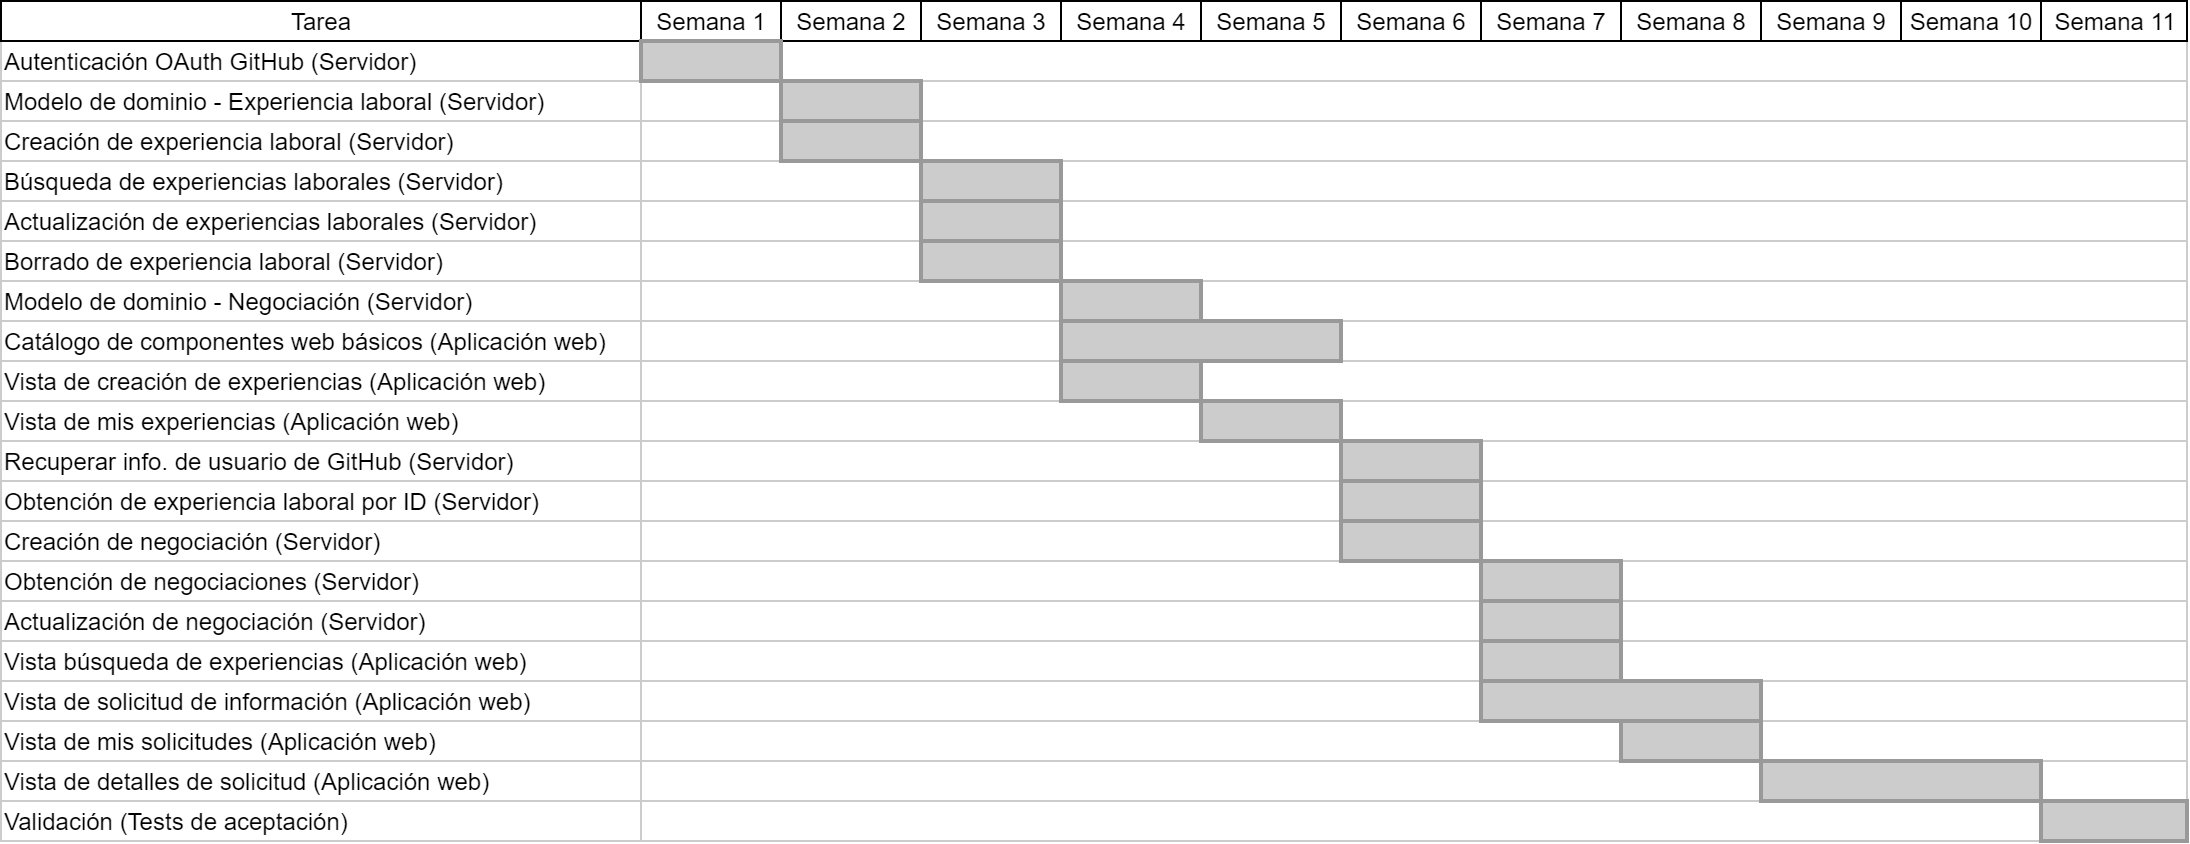
\includegraphics[width=15cm, keepaspectratio]{img/Gantt.png}
        \caption{Diagrama de Gantt del desarrollo de la aplicación.}\label{figure:gantt}
    \end{figure}


%%%%%%%%%%%%%%%%%%%%%%%%%%%%%%%%%%%%%%%%%%%%%%%%%%%%%%%%%%%%%%%%%%%%%%%%%%%%%%%%
%%%%%%%%%%%%%%%%%%%%%%%%%%%%%%%%%%%%%%%%%%%%%%%%%%%%%%%%%%%%%%%%%%%%%%%%%%%%%%%%
% ESTADO DEL ARTE %
%%%%%%%%%%%%%%%%%%%%%%%%%%%%%%%%%%%%%%%%%%%%%%%%%%%%%%%%%%%%%%%%%%%%%%%%%%%%%%%%

    \cleardoublepage


    \chapter{Estado del arte}
    \label{chap:estado}


    \section{Servidor de aplicaciones}
    \label{sec:intro_applicationserver}

    Es la pieza de software que no se ejecuta en el navegador si no que es invocada desde este vía conexión HTTP.
    Su cometido en la aplicación es el de exponer recursos que ofrecen la información de los usuarios, es decir, sus experiencias laborales y solicitudes de manera controlada basada en la identidad de los usuarios.
    Para ello antes de ofrecer información al lado cliente comprueba la identidad del usuario que la solicita para aplicarle las reglas de visibilidad y presentar únicamente la información que,
    o bien es pública, o bien pertenece al solicitante, o bien tanto el solicitante como el propietario han accedido a compartir. Abajo se describirán los puntos principales relacionados con el servidor de aplicaciones.

    \subsection{Lenguaje y plataforma}
    \label{subsec:intro_applicationserver_languageandplatform}

    El lenguaje elegido para el desarrollo del servidor es Java. Java es un lenguaje de programación orientada objetos desarrollado por la compañía Sun Microsystems.
    Una de sus particularidades más importantes es la de poder ejecutarse en la máquina virtual de Java (JVM) que puede ser instalada en la gran mayoría de sistemas operativos,
    lo que proporciona a este lenguaje gran portabilidad entre distintas plataformas. La versión concreta de Java que se utilizó para el desarrollo fue la 11, que entre otras características da Java soporte para la programación funcional.

    El framework Java utilizado para la creación del servidor fue Spring, un framework Open Source que facilita el desarrollo de aplicaciones Java Enterprise Edition, que es a su vez una plataforma, parte de la plataforma Java que permite el desarrollo de aplicaciones servidor.
    Spring Framework provee una serie de características y librerías que ayudan al programador a centrarse en el desarrollo de la lógica que quiere implementar en su aplicación, abstrayéndose de conceptos de infraestructura que complican el desarrollo de servidores.
    Para esta aplicación se utilizó concretamente la tecnología Spring Boot que además reduce la cantidad de configuración necesaria para funcionamiento de una aplicación Spring.

    \subsection{Comunicación con el cliente}
    \label{subsec:intro_applicationserver_communicationwithclient}

    Para permitir a la parte cliente del navegador acceder la información laboral que reside en el servidor, la aplicación servidor expone un API REST.
    Un API REST es una interfaz accesible de forma remota vía protocolo HTTP donde la información se representa en forma de recurso, siendo estos recursos identificadores de los conceptos y entidades que alberga el servidor, que en el caso de este Trabajo Fin de Grado son las experiencias laborales y las solicitudes de información.
    En un API REST estos recursos son operables utilizando los propios métodos HTTP, a los que el estilo REST provee de semántica, interpretándose los verbos HTTP como operaciones de escritura, lectura, borrado y modificación. De esta forma un cliente web puede en este caso crear, borrar, leer y modificar experiencias laborales y solicitudes dentro del servidor enviando mensajes HTTP.

    \subsection{Base de datos}
    \label{subsec:intro_applicationserver_database}

    Para almacenar las experiencias laborales de los usuarios y solicitudes, el servidor hace uso de una base de datos relacional (SQL), concretamente H2, que es un motor de bases de datos Open Source cuyas características principales son estar implementado en Java,
    lo que simplifica en muchos casos la integración con aplicaciones Java, y el poder levantarse en memoria o en modo embebido, de forma que sus datos se almacenan en ficheros, lo que facilita la base de desarrollo, evitando al programador tener que instalar y configurar una base de datos completa.
    El dialecto SQL que utiliza H2 es altamente compatible con el resto de dialectos de SQL, lo que a futuro permite hacer uso de otro distribuidor distinto de base de datos sin realizar grandes modificaciones.

    Como librería para realizar operaciones de base de datos desde el servidor se ha hecho uso de MyBatis, una herramienta de persistencia de Java que permite definir sentencias SQL en archivos XML que pueden ser invocadas desde el código y que integra fácilmente con Spring Framework.

    La herramienta para definir la estructura de la base de datos es Flyway, una tecnología que permite llevar un versionado de la base de datos mediante una lista de scripts SQL, uno por versión. Estos scripts se ejecutan secuencialmente, por lo que cada script debe escribirse como una modificación del estado de la estructura de base de datos que dejó el script anterior.
    De esta manera Flyway es capaz de llevar un registro de que modificaciones se hicieron en anteriores desarrollos sobre el proyecto, para ejecutar solo los nuevos scripts, es decir, los últimos cambios, no teniendo que generar una estructura nueva en cada modificación, lo que facilita la modificación de la base de datos una vez la aplicación está en producción,
    sin la pérdida de datos que supondría eliminar toda la estructura SQL y volverla a crear en cada modificación.


    \section{Aplicación web}
    \label{sec:intro_webapplication}

    Es la aplicación que se ejecuta en el navegador web del usuario. Su función es la de ofrecer una interfaz amigable e intuitiva al usuario para permitirle operar sobre sus recursos en el servidor y realizar consultas de datos.
    En el caso concreto de este Trabajo Fin de Grado, la aplicación web ofrece una interfaz para que el usuario pueda crear, modificar e eliminar sus experiencias laborales, realizar búsquedas de experiencias laborales mediante filtros
    y crear solicitudes de datos confidenciales a otros usuarios desde su navegador, mediante una interfaz gráfica.

    \subsection{Lenguaje y librerías}
    \label{subsec:intro_webapplication_languageandlibraries}

    El lenguaje utilizado para desarrollar la lógica en esta parte fue JavaScript. Este es un lenguaje interpretado orientado a objetos, que se ejecuta en los navegadores y permite modificar el documento HTML que visualiza el usuario, solicitar datos remotos a un servidor y almacenar datos en el propio navegador entre otras funciones.

    La librería utilizada para el desarrollo de la aplicación fue React, una librería que facilita el desarrollo de aplicaciones JavaScript de una sola página, cuya característica principal es la facilidad que aporta a la hora de desarrollar componentes web, es decir,
    componentes reutilizables en la aplicación, que se pueden invocar múltiples veces en el código mediante una etiqueta y atributos que actúan como entrada de información en el componente, y que tienen su propia estructura interna, comportamiento y estilo.
    Para esto React hace uso de archivos JavaScript con una extensión específica, JSX, que permiten referenciar HTML directamente desde el código JavaScript como si se tratara de un tipo de dato adicional a los que el JavaScript nativo soporta.
    Debido al uso de esta librería, la presencia de archivos HTML en la aplicación web es mínima, limitándose a un único archivo prácticamente vacío cuya función es referenciar los recursos necesarios para la ejecución de la aplicación.

    \subsection{Estilo}
    \label{subsec:intro_webapplication_style}

    Para agregar estilos a la interfaz gráfica y hacer la aplicación visualmente más atractiva se ha hecho uso de la librería Bootstrap. Bootstrap provee una serie de estilos CSS predefinidos y fácilmente utilizables sobre los elementos HTML de la aplicación en forma de clases HTML.


    \section{Autenticación}
    \label{sec:intro_authentication}

    Con el objetivo de facilitar a los usuarios el ingreso en la aplicación, esta se ha integrado con la plataforma GitHub, haciendo uso de ella como proveedora de autenticación e identidad. De esta manera, los usuarios que ya están registrados en GitHub, como suele ser el caso de los alumnos de carreras relacionadas con las TIC, pueden utilizar sus credenciales de GitHub para acceder a la aplicación. Estas credenciales se envían directamente a GitHub, por lo que no pasan directamente por la aplicación de este Trabajo Fin de Grado, de forma que en ningún momento se pone en riesgo la privacidad del usuario.

    Para lograr esto se ha hecho uso del módulo Spring Social, que facilita la comunicación con GitHub vía el estándar OAuth2, una forma de integrar aplicaciones con plataformas que ofrecen parte de los datos de sus usuarios sin vulnerar su privacidad, extendiendo la sesión de estos usuarios a aplicaciones de terceros.


    \section{Herramientas}
    \label{sec:intro_tools}
    A continuación se exponen brevemente algunas de las principales herramientas que se utilizaron para el desarrollo de la aplicación.

    \subsection{IntelliJ IDEA}
    \label{subsec:intro_tools_intellij}
    IntelliJ IDEA es un entorno de desarrollo integrado desarrollado por la compañía JetBrains. Tiene soporte para el lengauje Java, facilita las tareas de escritura del código, permite ejecutar y depurar aplicaciones y pruebas, integra con varias herramientas de gestión de dependencias y control de versiones, entre otras características. Se eligió este IDE para hacer el desarrollo del servidor de aplicaciones.

    \subsection{Visual Studio Code}
    \label{subsec:intro_tools_vsc}
    Visual Studio Code es un editor de código fuente con gran soporte para JavaScript. Permite ejecutar y depurar aplicaciones y pruebas, integra con gestores de dependencias y control de versiones. Se eligió este editor para el desarrollo de la aplicación web en React.

    \subsection{Maven}
    \label{subsec:intro_tools_maven}
    Maven es una herramienta de gestión de proyectos de software desarrollada por Apache Software Foundation. Permite de forma declarativa gestionar todas las dependencias de un proyecto Java, es decir, referenciar los módulos que contienen las librerías sobre las que se construye el proyecto para poder descargarlos automáticamente del repositorio central de Maven
    durante la construcción de la aplicación. También permite la ejecución de plugins que facilitan tareas de desarrollo como construcción, ejecución de pruebas, empaquetado, instalación, etcétera. Se utilizó para la gestión de dependecias del servidor de aplicaciones.

    \subsection{NPM}
    \label{subsec:intro_tools_npm}
    NPM es el sistema de gestión de paquetes para el lenguaje JavaScript. De forma similar a Maven permite gestionar las dependencias de una aplicación web JavaScript declarándolas en un fichero y automatizando de esta forma su descarga. Se utilizó para la gestión de dependencias de la aplicación web.

    \subsection{Git}
    \label{subsec:intro_tools_git}
    Git es un sistema de control de versiones distribuido y de código abierto. Permite mantener un histórico de los cambios del proyecto de forma remota (en este caso en Github) y una copia de estos de forma local. Además permite mantener distintas ramas de desarollo en paralelo, esta característica facilita el desarollo de distintas funcionalidades del software en paralelo, ya sea por uno o varios desarrolladores, siendo posible mezclar estas distintas ramas después con la versión final, gestionando mediante el sistema Git las diferencias y conflictos entre los cambios en el código.


    \section{Arquitectura hexagonal}
    \label{sec:intro_desc_hexagonal_arch}

    La arquitectura hexagonal, también denominada patrón de puertos y adaptadores, es un conjunto de patrones aplicados en el lado servidor de una aplicación
    que proporcionan una división en la aplicación en una serie de capas concéntricas con responsabilidades definidas.
    Esta división tiene como objetivo separar la lógica de negocio de una aplicación de las tecnologías utilizadas como consecuencia de la infrastructura en la que yace,
    es decir, bases de datos, buses de eventos, protocolos de transporte, etc. Algunas de las ventajas de esta arquitectura son:
    \begin{itemize}
        \item Las aplicaciones son más faciles de probar mediante pruebas cuyo alcance es
        solo una de las capas en cada caso, falseando las demás en el contexto de la prueba.
        \item Las aplicaciones son resilientes ante posibles cambios en la infrastructura, ya que en estos casos la lógica de negocio se mantiene sin modificar
        mientras que la adaptación solo dependerá de implementar nuevos adaptadores para las nuevas tecnologías de infrastructura.
        \item Resulta más fácil por otra parte evolucionar y modificar la lógica de negocio teniendo en cuenta que esta es totalmente independiente de las tecnologías
        de infrastructura y frameworks.
    \end{itemize}

    En la arquitectura hexagonal intervienen las siguientes capas:

    \begin{itemize}
        \item Modelo de dominio: Compuesto por las clases que representan los conceptos con los que el sistema opera.
        El modelo de dominio no debe tener dependencia con ninguna otra capa de la aplicación.
        Podemos distinguir las clases del modelo de dominio en dos tipos distintos:

        \begin{itemize}
            \item Entidades: son aquellas que son susceptibles de ser identificadas mediante un identificador único y que tienen ciclo de vida, es decir, evolucionan a lo largo del tiempo a través de las operaciones que los usuarios realizan sobre ellas.
            Podemos decir que dos entidades con igual información no son la misma entidad si difieren en su identificador único.
            Las entidades no son meras estructuras de datos anémicas, sino que continen la lógica necesaria para construirse, para cambiar de estado, para validar la información de la que se componen o la que transitan y para interoperar con otras entidades.
            Además son las propias entidades las que generan proyecciones de si mismas omitiendo datos en caso de que el usuario que las accede no tenga visibilidad sobre estos datos, por lo que son las encargadas de aplicar los criterios de privacidad.
            Desde este punto de vista podemos afirmar que las entidades contienen la lógica de negocio de la aplicación.
            \item Objetos de valor: representan tipos de datos del dominio de las experincias laborales que no tienen la capacidad de evolucionar a lo largo del tiempo, ya que de cambiar representarían realidades distintas. Se puede decir que dos objetos de valor con el mismo contenido son el mismo objeto de valor.
            Los objetos de valor tienen la capacidad de validarse en su construcción, de forma que no pueden construirse a partir de datos que no cumplan por ejemplo las restricciones de formato del objeto de valor.
        \end{itemize}

        \item Capa de aplicación: Es la capa del sistema que expone una interfaz de servicios que pueden invocarse para realizar las distintas operaciones que componen la funcionalidad de la aplicación. Además es la encargada de crear, persistir, recuperar y borrar las entidades del modelo de domino y de invocar su lógica de negocio.
        Es una aplicación Java pura, es decir, no requiere del framework, aunque puede utilizar librerías externas con un uso utilitario no requiere en este caso de contexto de Spring para funcionar, y solo depende de las clases del modelo de dominio.
        De este modo se logra que la lógica de negocio de la aplicación sea independiente de la infrastructura (protocolos de transporte, bases de datos, etcétera), haciendo el sistema fácilmente sea fácilmente acoplable a otras infrastructuras en caso de necesidad.
        Además permite realizar pruebas automáticas de lógica de negocio sin tener que levantar la infrastructura de la aplicación completa, de manera que son más descriptivas del comportamiento de la aplicación y más fáciles de mantener.
        Consta de los siguientes elementos:

        \begin{itemize}
            \item Interfaces de servicio: conocidas en la arquitectura como puertos primarios, son la entrada a la aplicación y representan el conjunto de operaciones que provee. Lo métodos de estas interfaces aceptan objetos denominados comandos en el caso de las operaciones de escritura, y denominados consultas en el caso de las operaciones de lectura.
            Las consultas y comandos contienen los objetos de valor necesarios para la ejecución del método de servicio al que se pasan como parámetros .
            \item Implementación de los servicios: Implementa la anterior interfaz, por lo que tiene el código necesario para ejecutar la lógica de las operaciones desde la entrada del comando o consulta hasta la invocación de la interfaz de repositorio, con la consiguiente vuelta de información.
            \item Interfaces de repositorio: conocidas en la arquitectura como puertos secundarios, proveen a la aplicación del juego de metódos para operar contra los sistemas donde se persisten las entidades, sean estas del dominio del sistema o no.
            Las implementaciones de las interfaces de repositorio no son objeto de la capa aplicación, por estar fuertemente acopladas a tecnologías de transporte y persistencia, por lo que pertenecen a la siguiente capa, la capa de infrastructura.
        \end{itemize}


        \item Capa de infrastructura: Es la capa del sistema que contiene el código que no está relacionado con la lógica de negocio sino con tecnologías de transporte y persistencia en base de datos, configuración y ejecución de la aplicación.
    \end{itemize}

%%%%%%%%%%%%%%%%%%%%%%%%%%%%%%%%%%%%%%%%%%%%%%%%%%%%%%%%%%%%%%%%%%%%%%%%%%%%%%%%
%%%%%%%%%%%%%%%%%%%%%%%%%%%%%%%%%%%%%%%%%%%%%%%%%%%%%%%%%%%%%%%%%%%%%%%%%%%%%%%%
% DISEÑO E IMPLEMENTACIÓN %
%%%%%%%%%%%%%%%%%%%%%%%%%%%%%%%%%%%%%%%%%%%%%%%%%%%%%%%%%%%%%%%%%%%%%%%%%%%%%%%%

    \cleardoublepage


    \chapter{Diseño e implementación}

    En este capítulo de describirá con detalle técnico el diseño e implementación de la aplicación completa desarrollada para este Trabajo Fin de Grado.


    \section{Arquitectura general}
    \label{sec:architecture_impl}

    Como se indicó anteriormente el sitema está compuesto por una aplicación web de navegador desarrollada en React y un servidor web desarrollado en Spring Boot.

    La aplicación web consiste en una única página web compuesta de componentes web de primer nivel, que denominamos vistas, y que contienen a su vez por componentes web de segundo nivel.
    Los componentes de primer nivel, llamados vistas, renderizan pantallas completas de la aplicación de una sola página, y tienen cada uno asociada una ruta de navegador.
    Los componentes de segundo nivel, renderizan elementos web reutilizables dentro de las distintas vistas, como entradas de texto, tarjetas, etcétera. En algunos casos un componente de segundo nivel puede hacer uso de otros componentes de segundo nivel para extender su funcionalidad.
    Además, la aplicación tiene un componente web de enrutado que permite navegar entre las distintas vistas, implementado con la tecnología React Router, que consiste en una barra de navegación horizontal en la parte superior de la pantalla.

    El servidor fue desarrollado siguiendo una arquitectura hexagonal.
    Podemos definir la aplicación de esta arquitectura al sistema implementado para este Trabajo Fin de Grado a partir de los elementos que la componen, más interno a más externo:

    \begin{itemize}
        \item Modelo de dominio:

        \begin{itemize}
            \item Entidades: En esta aplicación el dominio corresponde principalmente con los conceptos de experiencia laboral y negociación (también llamada solicitud de información), por lo tanto
            las entidades de este sistema son las experiencias laborales y las negociaciones.
            \item Objetos de valor: ejemplos de objetos de valor de nuestro sistema serían las empresas o las tecnologías, ya que podemos afirmar que dos empresas con distinto nombre son dos empresas distintas desde el punto de vista del sistema, al igual que ocurre con las tecnologías.
        \end{itemize}

        \item Capa de aplicación:

        \begin{itemize}
            \item Interfaces de servicio: ejemplos de servicios son el servicio de experiencias laborales y el servicio de negociaciones, por lo tanto la interfaz de servicios se compone de operaciones como creación, actulización, borrado y consulta de experiencias laborales,
            o creación, actualización, recuperación, aceptación o denegación de negociaciones.
            \item Interfaces de repositorio: ejemplos de repositorios del sistema son el de experiencias laborales y el de negociaciones, que operan contra la base de datos del sistema para persistir y recuperar estas entidades, o el repositorio de usuarios, que opera contra GitHub para recuperar información de usuarios vía conexión REST.
        \end{itemize}


        \item Capa de infrastructura:

        \begin{itemize}
            \item Spring Boot: utiliza clases de configuración que instancian en el contexto de Spring los bean necesarios para la ejecución de la aplicación.
            \item Spring MVC: define clases de tipo controlador que exponen endpoints invocables vía peticiones HTTP, estas clases conforman el API REST de la aplicación. También son las encargadas de, una vez deserializadas las peticiones HTTP, generar los comandos o consultas que serán enviados en la invocación a los puertos primarios de la aplicación.
            \item Spring Social: mediante configuración, levanta el mecanismo necesario para redireccionar a GitHub al usuario para ingresar en la aplicación, y una vez dentro permite acceder al contexto de seguridad de Spring para recuperar datos de la sesión como la identidad del usuario.
            \item Spring Template: con esta tecnología para realizar llamadas HTTP se implementa la interfaz de repositorio de usuarios, que realiza llamadas a GitHub.
            \item MyBatis: con esta tecnología para operar contra bases de datos SQL se implementan los repositorios de experiencias laborales y negociaciones.
        \end{itemize}

    \end{itemize}


    Para ilustrar el diseño de la arquitectura general de forma esquemática se incluye la Figura~\ref{fig:general_architecture} que refleja los elementos descritos anteriormente.

    \begin{figure}
        \centering
        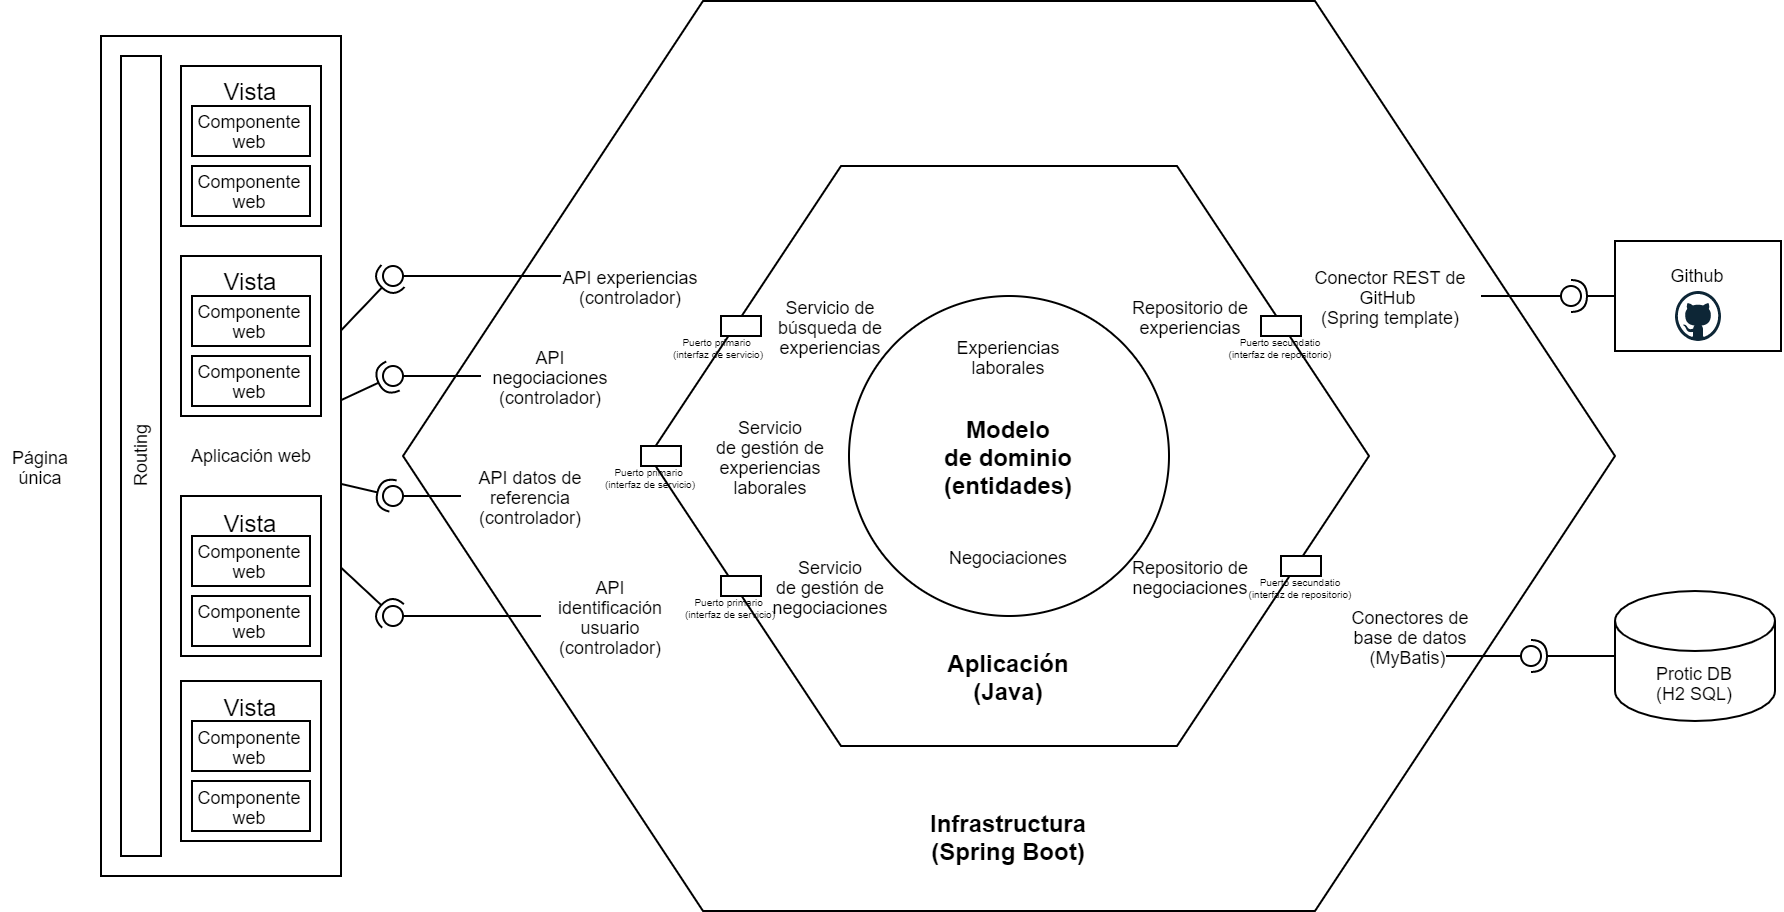
\includegraphics[width=15cm, keepaspectratio]{img/Arquitectura_hexagonal.png}
        \caption{Esquema de la arquitectura general.}\label{fig:general_architecture}
    \end{figure}


    \section{Modelo de dominio}
    \label{sec:domain_model_impl}
    A continuación se describe la implementación del modelo de dominio de la aplicación. Para ello esta sección se estructurará en cinco subsecciones:

    \begin{itemize}
        \item Clases e interfaces comunes: aquellas clases del modelo de dominio comunes a toda la aplicación.
        \item Objetos de valor del dominio de las experiencias laborales: clases de los objetos de valor relacionados con la entidad experiencia laboral.
        \item Entidad experiencia laboral: descripción de las clases e interfaces que constituyen la entidad experiencia laboral.
        \item Objetos de valor del dominio de las negociaciones: clases de los objetos de valor relacionados con la entidad negociación.
        \item Entidad negociación: descripción de las clases e interfaces que constituyen la entidad negociación.
    \end{itemize}

    Para ayudar a visualizar la implementación del modelo de dominio se han añadido las Figuras~\ref{fig:domain_model_vo} y~\ref{fig:domain_model_entities} que representan los objetos de valor y las entidades de la aplicación respectivamente.

    \begin{figure}
        \centering
        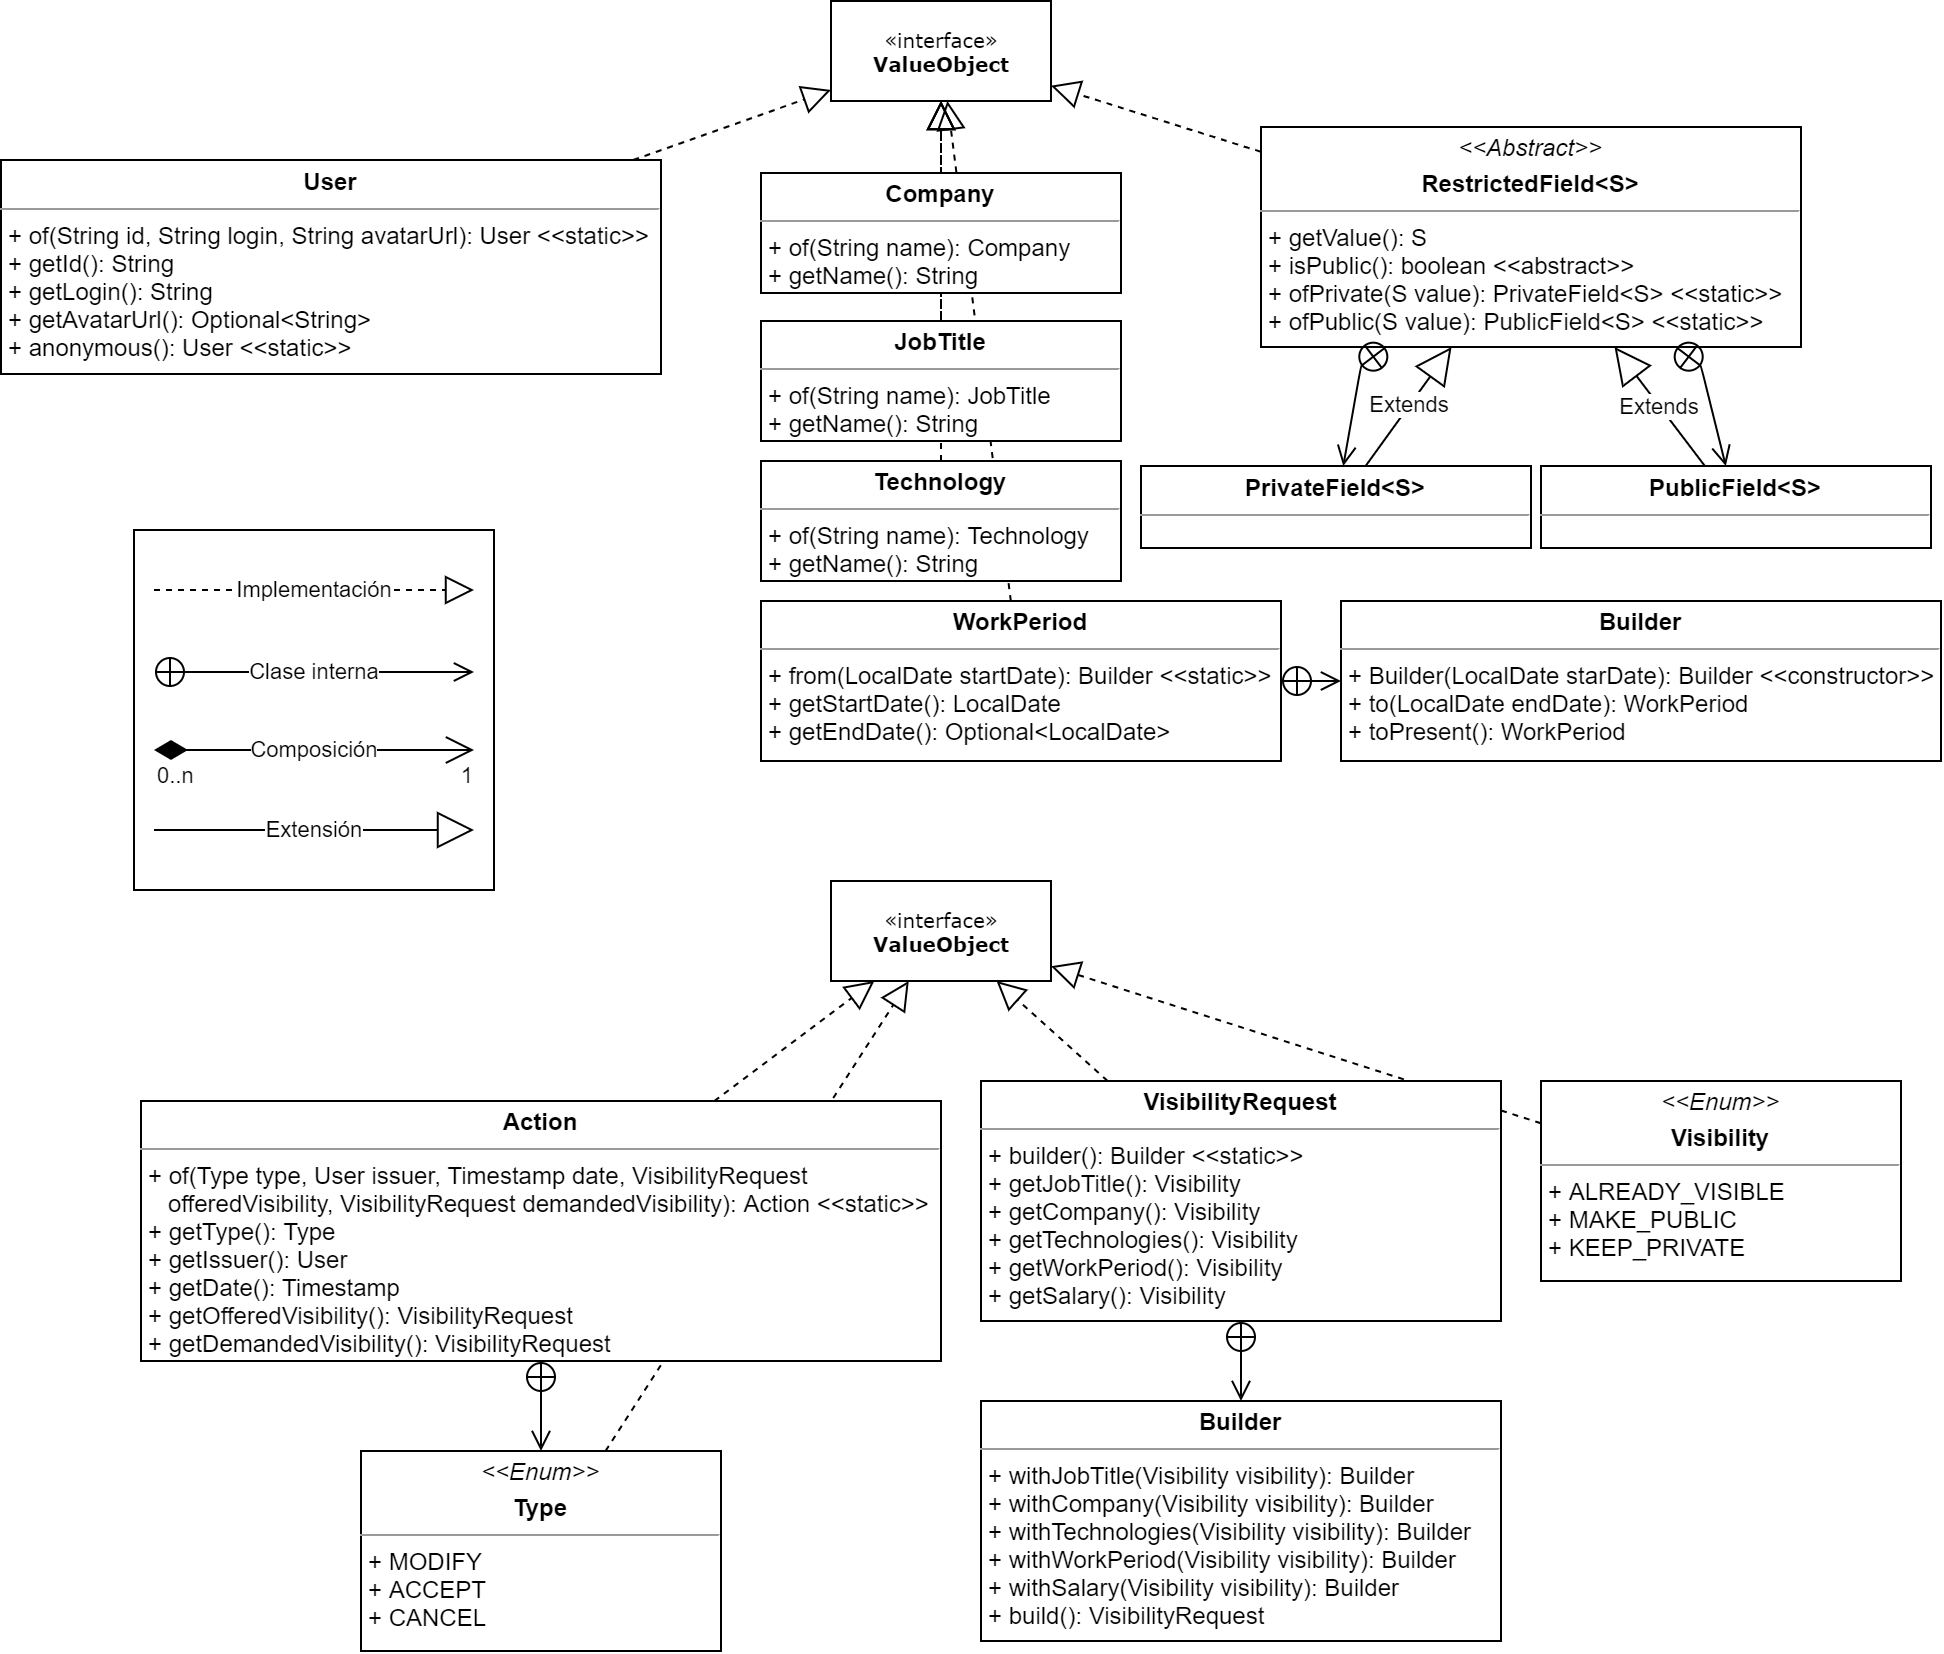
\includegraphics[width=15cm, keepaspectratio]{img/Modelo_dominio_vo.png}
        \caption{Representación de los objetos de valor del modelo de dominio.}\label{fig:domain_model_vo}
    \end{figure}

    \begin{figure}
        \centering
        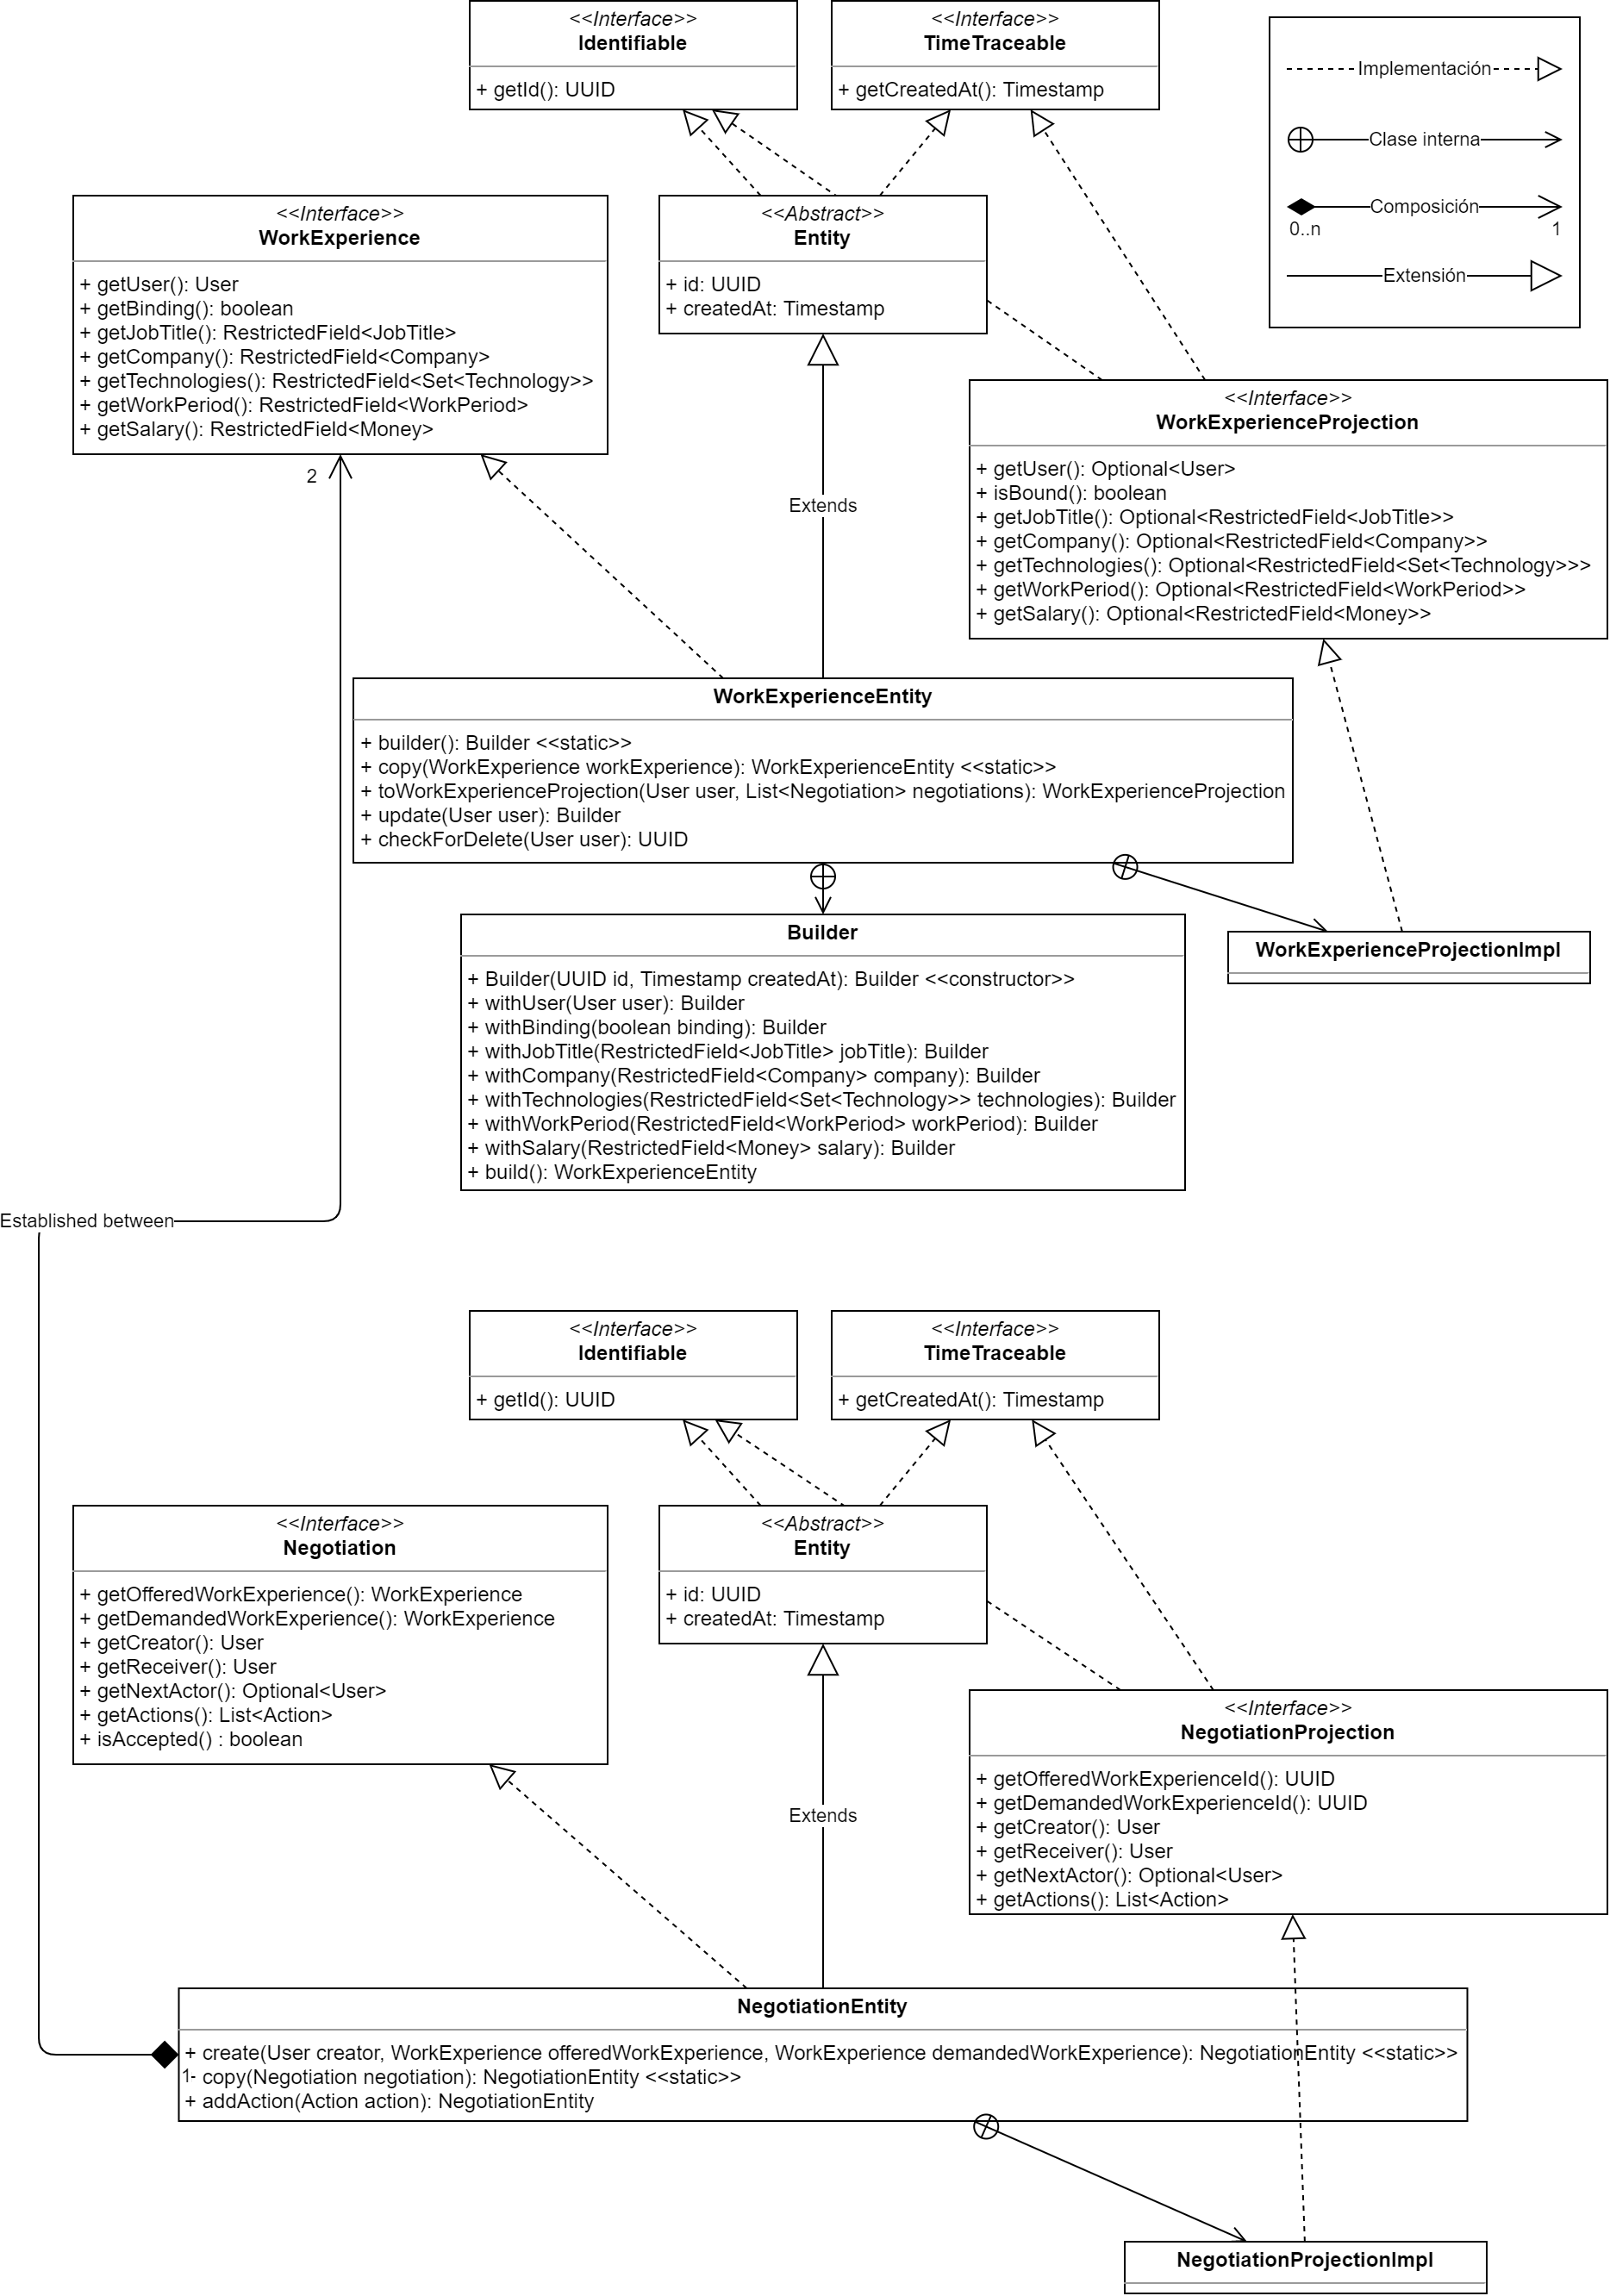
\includegraphics[width=15cm, keepaspectratio]{img/Modelo_dominio_entities.png}
        \caption{Representación de las entidades del modelo de dominio.}\label{fig:domain_model_entities}
    \end{figure}

    \subsection{Clases e interfaces comunes}
    \label{subsec:common_classes}
    Son las clases e interfaces utilizadas en todo el modelo de dominio de la aplicación. Se listan a continuación:

    \begin{itemize}
        \item \textbf{Identifiable:} Interfaz que implementan aquellas clases que se pueden identificar mediante un identificador único de tipo \emph{UUID}.
        \item \textbf{TimeTraceable:} Interfaz que implementan aquellas clases que tienen una fecha de creación.
        \item\textbf{Entity:} Clase abstracta que extienden todas las entidades del modelo de dominio. Puesto que las entidades son siempre identificables y su fecha de creación es relevante, esta clase implementa ambas interfaces \emph{Identifiable} y \emph{TimeTraceable}
        \item \textbf{ValueObject:} Interfaz que implementan aquellas clases que son objetos de valor, es decir, aquellas clases que representan tipos de datos inmutables. Esta interfaz no tiene funcionalidad, su propósito es únicamente semántico.
        \item \textbf{User:} Objeto de valor que representa a un usuario de la aplicación. Contiene como datos el idetificador del usuario en GitHub, su nombre de usuario y la URL de su avatar.
    \end{itemize}

    \subsection{Objetos de valor del dominio de las experiencias laborales}
    \label{subsec:work_experience_value_objects}
    Los objetos de valor del dominio de la experiencia laboral son clases que reprensetan aquellos tipos de datos estáticos de los que se compone la información de la experiencia laboral.
    Su propósito es doble, por una parte aportan semántica al tipado de los atributos de la entidad experiencia laboral, por otra facilitan implementar las validaciones necesarias para construir estos atributos.
    Se listan a continuación:

    \begin{itemize}
        \item \textbf{Company:} Representa la empresa donde tuvo lugar la experincia laboral.
        \item \textbf{JobTitle:} Representa el puesto de trabajo de la experiencia laboral.
        \item\textbf{Technology:} Representa una tecnología que se manejó dentro de una experiencia laboral.
        \item \textbf{WorkPeriod:} Representa un periodo laboral con fecha de inicio y que puede tener o no fecha de fin. Se construye a través de una clase \emph{Builder} que permite la creación de periodos laborales concluidos o que duran hasta la actualidad.
        \item \textbf{RestrictedField:} Es una clase genérica cuyo propósito es envolver a un objeto de valor de los tipos anteriores, añadiéndole en cada caso la visibilidad pública o privada. Para ello tiene dos extensiones llamadas \emph{PrivateField} y \emph{PublicField}.
        Se puede construir a partir de dos métodos estáticos que aceptan un objeto de valor como parámetro y devuelven un objeto de una de las dos extensiones que contiene al objeto de valor.
    \end{itemize}

    \subsection{Entidad experiencia laboral}
    \label{subsec:work_experience_entity}
    Aquí se describen las clases e interfaces que están relacionadas con el concepto de experiencia laboral como entidad de la aplicación:

    \begin{itemize}
        \item \textbf{WorkExperienceEntity:} Clase principal, representa directamente la entidad experiencia laboral.
        Se compone principalmente de una serie de atributos finales, estos atributos tienen como tipo uno de los objetos de valor de la experiencia laboral, pero envueltos como campos restringidos.
        Estos atributos, que pueden ser públicos o privados, son el nombre del puesto de trabajo, la empresa, la lista de tecnologías utilizadas, el periodo laboral y el salario. Adicionalmente esta entidad guarda la información del usuario al que pertenece, y su decisión de vincularla o no a su perfil.
        Esta entidad tiene en sus métodos la lógica de negocio necesaria para:
        \begin{itemize}
            \item Actualizar su información comprobando previamente que el usuario que la actualiza es dueño de la entidad experiencia laboral que trata de actualizar.
            \item Comprobar que un usuario que trata de borrar la entidad es dueño de esta para permitirlo o impedirlo en caso contrario.
            \item Generar una proyección de la propia entidad para un usuario concreto que trata de consultarla, con los campos que el usuario solicitante no tiene permiso para ver omitidos.
        \end{itemize}
        \item \textbf{WorkExperienceProjection:} Esta interfaz se devuelve en las consultas de experiencias laborales de la aplicación, en lugar de las propias entidades. Su utilidad es la de omitir todos aquellos atributos que el usuario solicitante no tiene permiso para ver. Para ello, la entidad genera proyecciones de este tipo siguiendo las siguientes reglas:
        \begin{itemize}
            \item Un atributo siempre es visible para el poseedor de la experiencia laboral.
            \item Un atributo es visible para cualquier usuario si es público.
            \item Un atributo privado solo es visible para un usuario que no sea poseedor de la entidad, si existe para esta entidad alguna negociación entre el solicitante y el poseedor en estado aceptado que habilite el atributo.
            \item El usuario poseedor de la entidad es siempre visible a sí mismo.
            \item El usuario poseedor de la entidad es solo visible para otros usuarios si vinculó la experiencia laboral a su perfil. En caso contrario se mostrará como anónimo.
        \end{itemize}
        \item \textbf{WorkExperience:} Esta interfaz es implementada por la entidad. Provee los métodos de acceso a sus atributos, pero no contiene los métodos de negocio de la entidad. De esta forma se impide que fuera de la capa de aplicación se trate de invocar métodos de negocio.
    \end{itemize}

    \subsection{Objetos de valor del dominio de las negociaciones}
    \label{subsec:negotiation_value_objects}
    Los objetos de valor del dominio de las negociaciones son clases que reprensetan aquellos tipos de datos estáticos que conforman una negociaciónl.
    Su propósito es contener la información relativa al histórico de la negociación y la visibilidad que los usuarios ofrecen y solicitan en relación a las experiencias laborales.
    Se listan a continuación:

    \begin{itemize}
        \item \textbf{Visibility:} Tipo enumerado que reprensenta un cambio de visibilidad sobre un campo. Tiene tres posibles valores:
        \begin{itemize}
            \item \textbf{MAKE\_PUBLIC:} En relación a un campo de una experiencia laboral indica que se solicita que se convierta en público.
            \item \textbf{KEEP\_PRIVATE:} En relación a un campo de una experiencia laboral indica que no se solicita que el campo se convierta en público, sino que se mantenga privado.
            \item \textbf{ALREADY\_VISIBLE:} En relación a un campo de una experiencia laboral indica que el campo ya era público previamente a la negociación.
        \end{itemize}
        \item \textbf{VisibilityRequest:} Representa una solicitud de visibilidad sobre una experiencia laboral. Contiene un atributo por campo de la experiencia laboral, de tipo \emph{Visibility} indicando que política de visibilidad se quiere establecer sobre el campo.
        \item \textbf{Action:} Representa una acción en el histórico de una negociación. Las acciones pueden ser de tipo \emph{modificación, aceptación y cancelación} en función de si modifican la negociación o la aceptan o cancelan.
        Cada acción tiene una referencia al usuario que la ejecuta.
        Cada acción tiene ligadas la oferta de visibilidad sobre la experiencia laboral ofrecida y la solicitud de visibilidad sobre la oferta laboral solicitada, ambas del tipo \emph{VisibilityRequest}.
    \end{itemize}

    \subsection{Entidad negociación}
    \label{subsec:negotiation_entity}
    Aquí se describen las clases e interfaces que están relacionadas con el concepto de negociaciónl como entidad de la aplicación:

    \begin{itemize}
        \item \textbf{NegotiationEntity:} Clase principal, representa directamente la entidad negociación.
        Se compone de:
        \begin{itemize}
            \item La referencia al usuario creador de la negociación.
            \item La referencia al usuario receptor de la negociación.
            \item La experiencia laboral que el usuario creador de la negociación ofreció.
            \item La experiencia laboral que el usuario creador de la negociación solictó al usuario receptor.
            \item El histórico de acciones que sucedieron durante la negociación.
            \item La referencia al usuario que debe dar el siguiente paso en la negociación si esta está activa.
        \end{itemize}
        Esta entidad tiene en sus métodos la lógica de negocio necesaria para comprobar que un usuario que añade una acción a la negociación tiene permiso para hacerlo, comprobando si es el siguiente actor de la negociación.
        \item \textbf{NegotiationProjection:} Esta interfaz se devuelve en las consultas de negociaciones de la aplicación, en lugar de las propias entidades.
        Su utilidad es la de omitir todas las referencias de la negociación a un usuario cuando este no tiene vinculada con su perfil la experiencia laboral sobre la que se estable la negociación, de forma que el otro usuario no pueda conocer en ningún momento su identidad mientras negocia con él.
        \item \textbf{Negotiation:} Esta interfaz es implementada por la entidad. Provee los métodos de acceso a sus atributos, pero no contiene los métodos de negocio de la entidad. De esta forma se impide que fuera de la capa de aplicación se trate de invocar métodos de negocio.
    \end{itemize}


    \section{Modelo de datos}
    \label{sec:data_model}
    Para explicar el modelo de datos de la aplicación se dará una breve descripción de cada una de las tablas que lo componen. La explicación se apoyará en el diagrama de la Figura~\ref{fig:data_model}

    \begin{figure}
        \centering
        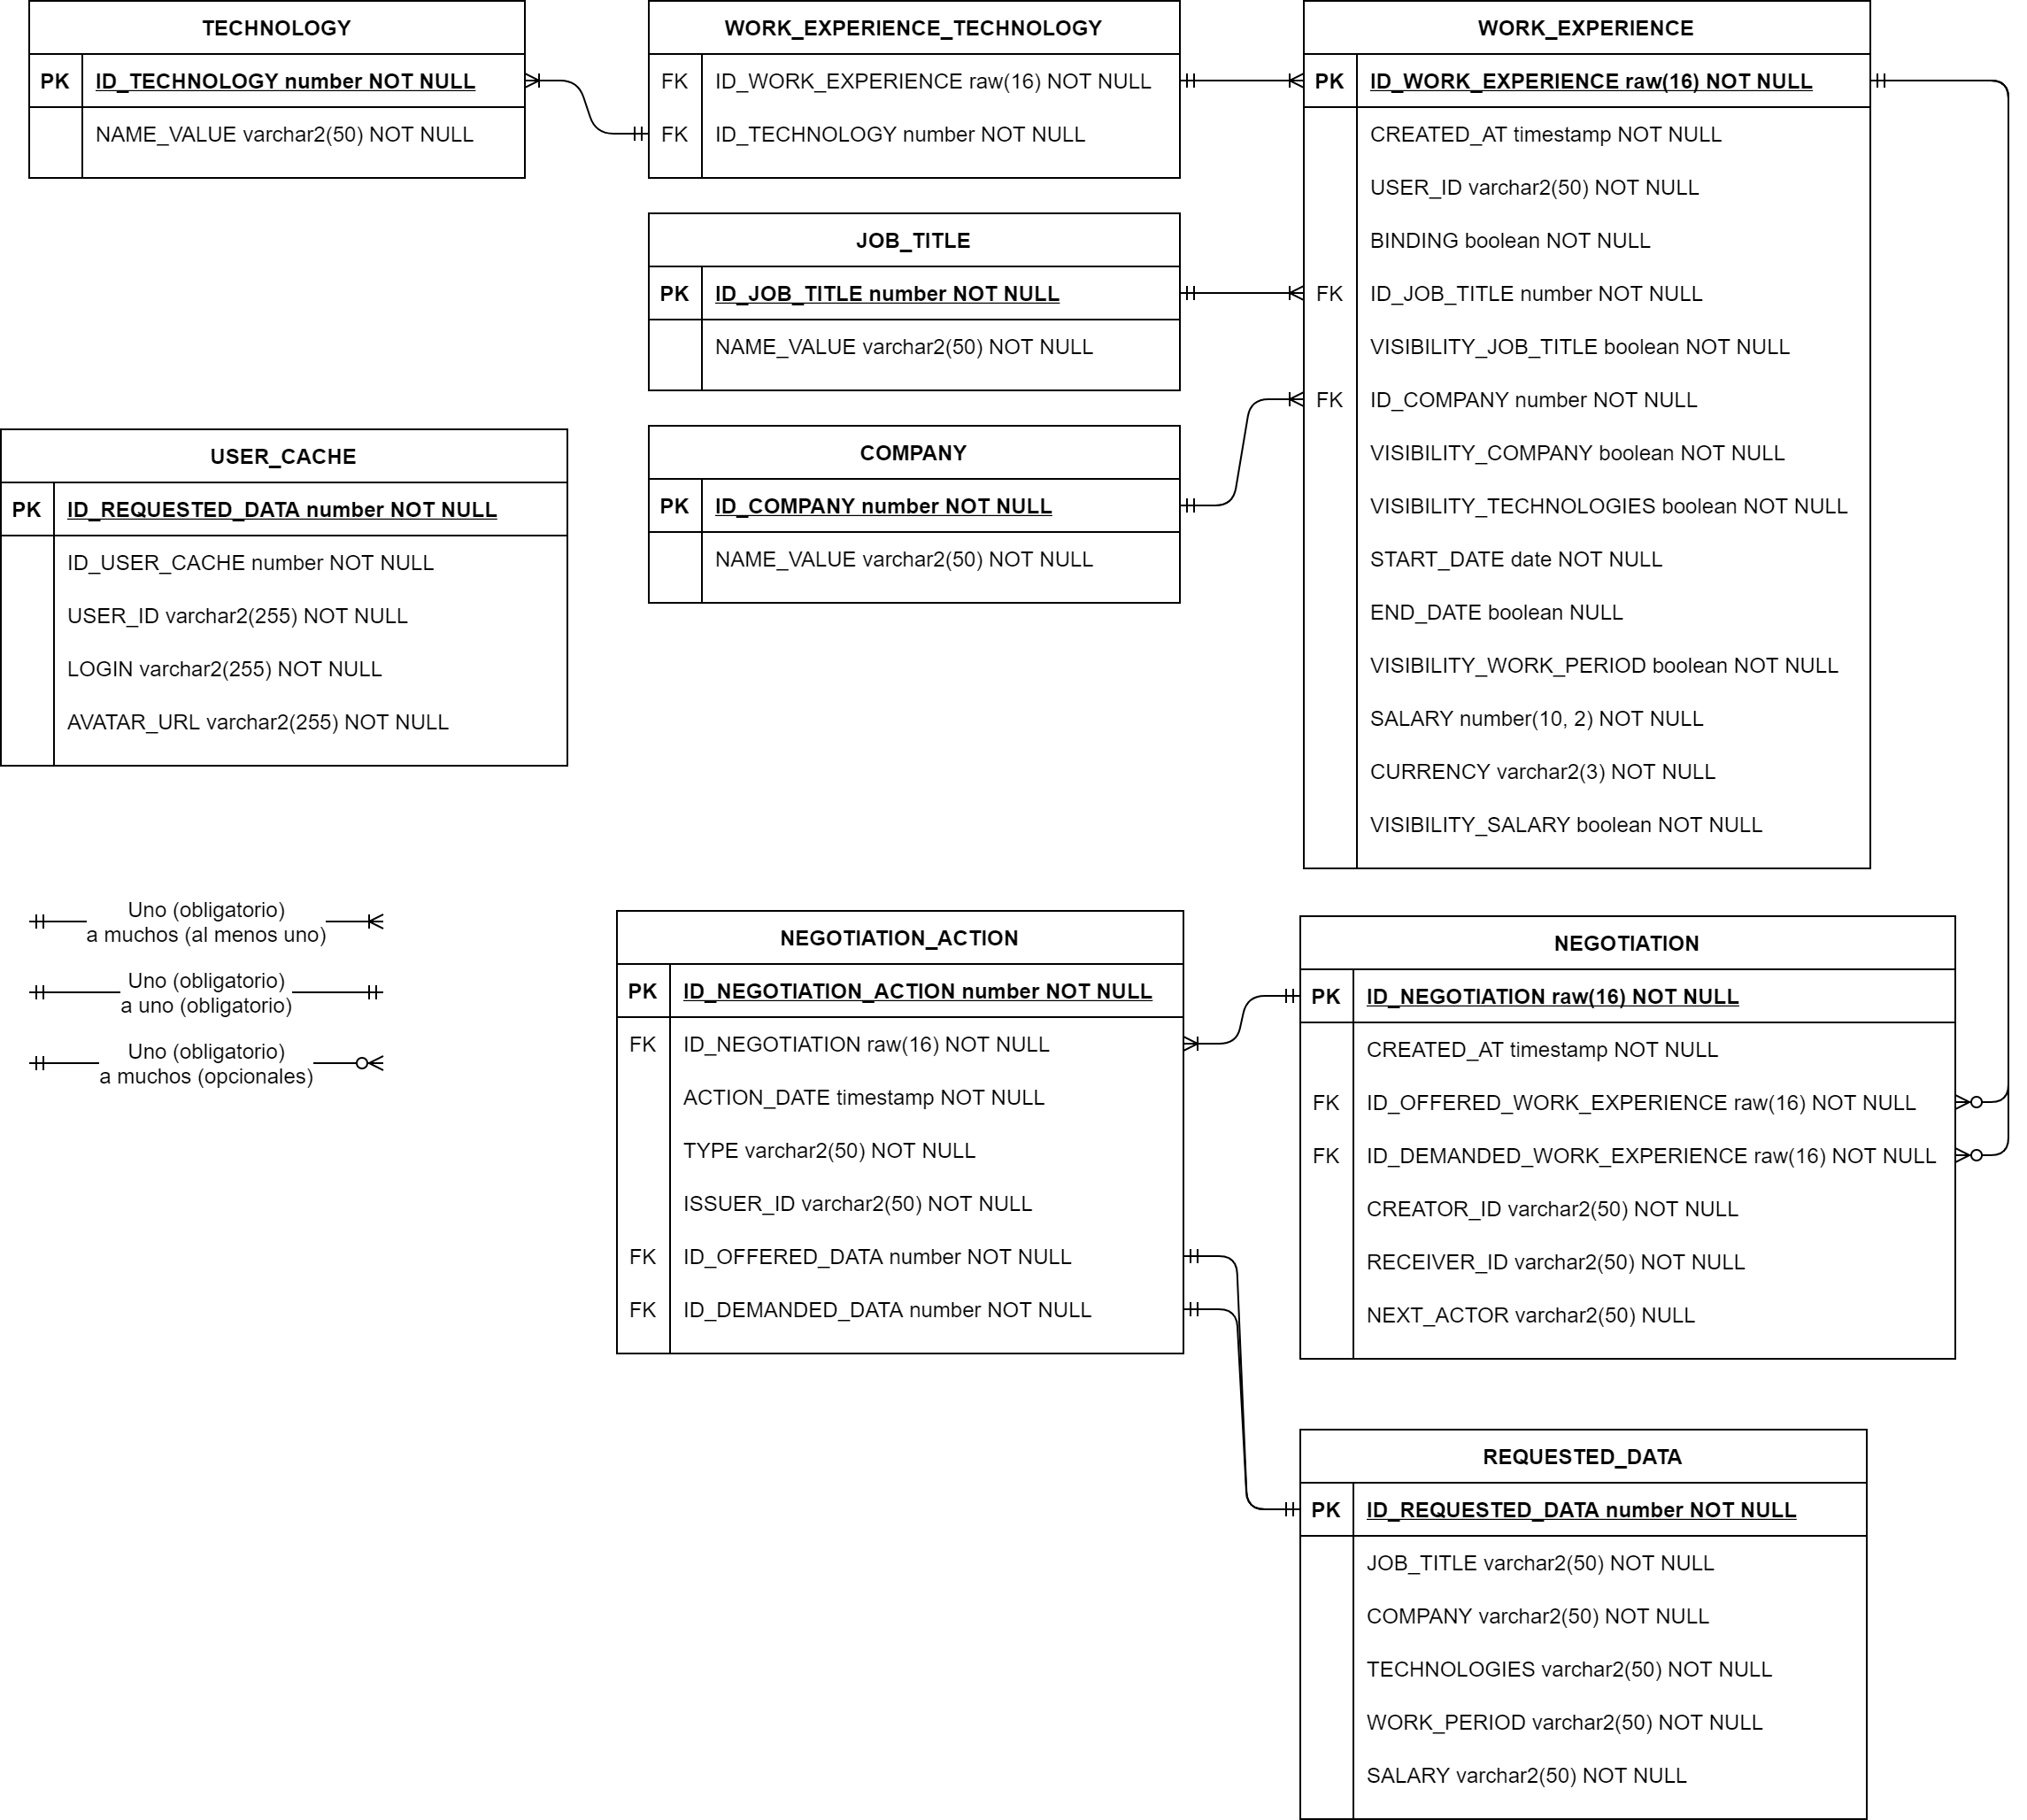
\includegraphics[width=15cm, keepaspectratio]{img/Modelo_datos.png}
        \caption{Diagrama de entidad relación del modelo de datos.}\label{fig:data_model}
    \end{figure}


    \begin{itemize}
        \item \textbf{Tabla WORK\_EXPERIENCE:} En ella se alamacenan los datos relativos a cada experiencia laboral perteneciente a los usuarios.
        Contiene el identificador único de la experiencia laboral, su fechar de creación, el identificador del usuario al que pertenece la experiencia, el indicador de si la experiencia extá vinculada o no al perfil del usuario.
        Además, para cada campo de la experiencia laboral, esta tabla contiene:
        \begin{itemize}
            \item Puesto de trabajo: la visibilidad (privada o pública) del campo y una referencia a la tabla \emph{JOB\_TITLE} que contiene el puesto de trabajo.
            \item Empresa: la visibilidad (privada o pública) del campo y una referencia a la tabla \emph{COMPANY} que contiene el nombre de la empresa.
            \item Tecnologías: la visibilidad (privada o pública) del campo. La tabla \emph{WORK\_ EXPERIENCE\_TECHNOLOGY} puede contener varias referencias a esta tabla, una por tecnología asociada a la experiencia laboral.
            \item Período laboral: la visibilidad (privada o pública) del campo y las fechas de inicio y fin de la experiencia laboral, siendo la última nula si la experiencia dura hasta la actualidad.
            \item Salario: la visibilidad (privada o pública) del campo y la cuantía del salario bruto anual, además del código ISO de la moneda.
        \end{itemize}
        \item \textbf{Tabla JOB\_TITLE:} Contiene los nombres de los puestos de trabajo relacionados con las experiencias laborales.
        \item \textbf{Tabla COMPANY:} Contiene los nombres de las empresas relacionadas con las experiencias laborales.
        \item \textbf{Tabla WORK\_EXPERIENCE\_TECHNOLOGY:} Relaciona las experincias laborales con las tecnologías utilizadas en cada una de ellas, mediante una relación de muchas a muchas.
        \item \textbf{Tabla TECHNOLOGY:} Contiene los nombres de las tecnologías relacionadas con las experiencias laborales.
        \item \textbf{Tabla NEGOTIATION:} En ella se almacenan los datos relativos a las negociaciones.
        Contiene el identificador único de la negociación, su fecha de creación, una referencia a la experiencia laboral ofrecida en la negociación y otra a la experiencia laboral solicitada, el identificador del usuario creador de la negociación y del usuario receptor, y el identificador del usuario que será el siguiente actor en la negociación, si aplica.
        \item \textbf{Tabla NEGOTIATION\_ACTION:} En ella se almacena el histórico de acciones que han ido transcurriendo para cada negociación.
        Cada registro contiene la referencia a la negociación sobre la que se aplicó la acción, la fecha en la que se aplicó, el tipo de acción (modificación, aceptación o cancelación), el identificador del usuario que realizó la acción,
        y las referencias a la tabla \emph{REQUESTED\_DATA} donde se almacenan la visibilidad a aplicar a cada uno de los campos de la experiencia ofrecida y de la experiencia solicitada.
        \item \textbf{Tabla REQUESTED\_DATA:} En ella se almacenan los posibles valores de la visibilidad de los campos para una experiencia laboral en negociación, siendo estos "manetener privado", "hacer público" o "ya público".
        \item \textbf{Tabla USER\_CACHE:} En esta tabla se almacena la información de los usuarios que se obtiene de GitHub, para evitar realizar peticiones HTTP para información de usuarios que ya se ha obtenido en el pasado.
    \end{itemize}


    \section{Diseño del API}
    \label{sec:api_desing}
    En esta sección se describirá el API REST de la aplicación en cuatro grupos de puntos de API según su clasifiación funcional:

    \begin{itemize}
        \item Puntos de API de sesión: aquellos relacionados con la sesión del usuario.
        \item Puntos de API de datos de referencia: aquellos que se utilizan para consultar puestos de trabajo, empresas y tecnologías que ya se dieron de alta en la aplicación.
        \item Puntos de API de experiencias laborales: aquellos relacionados con operaciones sobre la entidad experiencia laboral.
        \item Puntos de API de negociaciones: aquellos relacionados con operaciones sobre la entidad negociación.
    \end{itemize}

    \subsection{Puntos de API de sesión}
    \label{subsec:session_endpoints}
    Es el conjunto de dos puntos de API que proveen operaciones relacionadas con la sesión del usuario:

    \subsubsection{Punto de API de obtención de usuario}
    \label{subsec:get_user}
    Este punto de API se utiliza para obtener la información del usuario que encuentra en sesión.
    Las solicitudes se envían metidante el método \emph{GET} al recurso de la aplicación \emph{/user}.
    A continuación se muestra un ejemplo de llamada al punto de API:

        {\footnotesize
    \begin{verbatim}
			-- Solicitud
			GET /user

			-- Respuesta
			200 OK
			{
			    "id": "1",
			    "login": "mojombo",
			    "avatarUrl": "https://avatars.githubusercontent.com/u/1?v=4"
			}
    \end{verbatim}
    }

    \subsubsection{Punto de API de cierre de sesión}
    \label{subsec:get_user}
    Este punto de API se utiliza para invalidar la sesión del usuario en un cierre de sesión.
    Las solicitudes se envían metidante el método \emph{GET} al recurso de la aplicación \emph{/user/logout}.
    A continuación se muestra un ejemplo de llamada al punto de API:

        {\footnotesize
    \begin{verbatim}
			-- Solicitud
			GET /user/logout

			-- Respuesta
			200 OK
    \end{verbatim}
    }

    \subsection{Puntos de API de datos de referencia}
    \label{subsec:reference_endpoints}
    Es el conjunto de tres puntos de API que se utilizan para proveer listados de información preexistente para las experencias laborales.
    Se utilizan principalmente para alimentar componentes de tipo combo en la interfaz de usuario:

    \subsubsection{Punto de API de datos de puesto de trabajo}
    \label{subsec:get_data_job_titles}
    Este punto de API se utiliza para obtener la lista de nombres de puestos de trabajo que ya existen en la aplicación.
    Las solicitudes se envían metidante el método \emph{GET} al recurso de la aplicación \emph{/data/job-titles}.
    La solicitud acepta un parámetro de consulta llamado \emph{name} cuyo valor permite filtrar aquellos elementos de la lista que lo contienen en su nombre:
    A continuación se muestra un ejemplo de llamada al punto de API:

        {\footnotesize
    \begin{verbatim}
			-- Solicitud
			GET /data/job-titles?name=pro

			-- Respuesta
			200 OK
			{
			    "data": [
			        "ANALISTA/PROGRAMADOR",
			        "DISEÑADOR DE PROCESOS",
			        "PRODUCT OWNER",
			        "PROGRAMADOR"
			    ]
			}
    \end{verbatim}
    }

    \subsubsection{Punto de API de datos de empresas}
    \label{subsec:get_data_companies}
    Este punto de API se utiliza para obtener la lista de nombres de empresas que ya existen en la aplicación.
    Las solicitudes se envían metidante el método \emph{GET} al recurso de la aplicación \emph{/data/companies}.
    La solicitud acepta un parámetro de consulta llamado \emph{name} cuyo valor permite filtrar aquellos elementos de la lista que lo contienen en su nombre:
    A continuación se muestra un ejemplo de llamada al punto de API:

        {\footnotesize
    \begin{verbatim}
			-- Solicitud
			GET /data/companies?name=in

			-- Respuesta
			200 OK
			{
			    "data": [
			        "ARQUIMEA INGENIERÍA",
			        "INDRA",
			        "ING"
			    ]
			}
    \end{verbatim}
    }

    \subsubsection{Punto de API de datos de tecnologías}
    \label{subsec:get_data_job_technologies}
    Este punto de API se utiliza para obtener la lista de nombres de tecnologías que ya existen en la aplicación.
    Las solicitudes se envían metidante el método \emph{GET} al recurso de la aplicación \emph{/data/technologies}.
    La solicitud acepta un parámetro de consulta llamado \emph{name} cuyo valor permite filtrar aquellos elementos de la lista que lo contienen en su nombre:
    A continuación se muestra un ejemplo de llamada al punto de API:

        {\footnotesize
    \begin{verbatim}
			-- Solicitud
			GET /data/technologies?name=j

			-- Respuesta
			200 OK
			{
			    "data": [
			        "DJANGO",
			        "JAVA",
			        "JAVA 11",
			        "JAVASCRIPT",
			        "JQUERY",
			        "VUE JS"
			    ]
			}
    \end{verbatim}
    }

    \subsection{Puntos de API de experiencias laborales}
    \label{subsec:work_experience_endpoints}
    Es el conjunto de dos puntos de API que proveen operaciones sobre la entidad experiencia laboral.

    \subsubsection{Punto de API de creación de experiencia laboral}
    \label{subsec:post_work_experience}
    Este punto de API se utiliza para crear una nueva experiencia laboral.
    Las solicitudes se envían metidante el método \emph{POST} al recurso de la aplicación \emph{/work-experience}.
    El cuerpo de la solicitud contiene la información acerca de la experiencia laboral a crear en formato JSON.
    La respuesta contiene el identificador único de la nueva experiencia laboral.
    A continuación se muestra un ejemplo de llamada al punto de API:

        {\footnotesize
    \begin{verbatim}
			-- Solicitud
			POST /work-experience
			{
			    "binding": true,
			    "jobTitle": {
			        "public": true,
			        "content": "Analista/Desarrollador"
			    },
			    "company": {
			        "public": true,
			        "content": "Indra"
			    },
			    "technologies": {
			        "public": true,
			        "content": [
			            "Java",
			            "Spring"
			        ]
			    },
			    "workPeriod": {
			        "public": true,
			        "content": {
			            "startDate": "2020-04-10",
			            "endDate": "2021-04-11"
			        }
			    },
			    "salary": {
			        "public": true,
			        "content": {
			            "value": 36000,
			            "currency": "EUR"
			        }
			    }
			}

			-- Respuesta
			200 OK
			{
			    "id": "99784c87-70d0-43cc-a340-aa28a19cb8a3"
			}
    \end{verbatim}
    }

    \subsubsection{Punto de API de obtención de experiencia laboral por identificador}
    \label{subsec:get_work_experience_id}
    Este punto de API se utiliza para recuperar una experiencia laboral por su identificador único.
    Las solicitudes se envían metidante el método \emph{GET} al recurso de la aplicación \emph{/work-experience/\{id\}}, donde \emph{id} es el identificador de la experiencia laboral a recuperar.
    La respuesta contiene los datos de la experiencia laboral, con los filtros de visibilidad aplicados según el usuario solicitante.
    A continuación se muestra un ejemplo de llamada al punto de API:

        {\footnotesize
    \begin{verbatim}
			-- Solicitud
			GET /work-experience/99784c87-70d0-43cc-a340-aa28a19cb8a3

			-- Respuesta
			200 OK
			{
			    "id": "99784c87-70d0-43cc-a340-aa28a19cb8a3",
			    "user":{
			        "id": "5689851",
			        "login": "vicengg",
			        "avatarUrl": "https://avatars.githubusercontent.com/u/5689851?v=4"
			    },
			    "binding": true,
			    "jobTitle":{
			        "content": "ANALISTA/DESARROLLADOR",
			        "public": true
			    },
			    "company":{
			        "content": "INDRA",
			        "public": true
			    },
			    "technologies":{
			        "content":[
			            "JAVA",
			            "SPRING"
			        ],
			        "public": true
			    },
			    "workPeriod":{
			        "content":{
			            "startDate": "2020-04-10",
			            "endDate": "2021-04-11"
			        },
			        "public": true
			    },
			    "salary":{
			        "content":{
			            "value": 3.6E+4,
			            "currency": "EUR"
			        },
			        "public": true
			    }
			}
    \end{verbatim}
    }

    \subsubsection{Punto de API de búsqueda de experiencias laborales}
    \label{subsec:get_work_experience}
    Este punto de API se utiliza para buscar experiencias laborales filtrando por su contenido.
    Las solicitudes se envían metidante el método \emph{GET} al recurso de la aplicación \emph{/work-experience}.
    La solicitud admite varios parámetros de consulta que filtran el resultado:
    \begin{itemize}
        \item \emph{scope}: Indica si se solicitan todas las experiencias laborales (\emph{scope=all}), las del usuario (\emph{scope=own}) o las del resto de usuarios (\emph{scope=foreign}).
        Su valor por defecto es \emph{all}.
        \item \emph{jobTitle}: Al asignar un cadena de caracteres a este filtro, solo se devolveran aquellas experiencias que contengan esa en el nombre del puesto de trabajo.
        \item \emph{company}: Al asignar un cadena de caracteres a este filtro, solo se devolveran aquellas experiencias que contengan esa en el nombre de la empresa.
        \item \emph{technologies}: Al asignar múltiples cadenas de caracteres a este filtro, solo se devolveran aquellas experiencias que contengan esas cadenas en su lista de tecnologías.
        \item \emph{startDate}: Enviar este filtro hará que solo las experiencias laborales que iniciaron después de la fecha indicada estén presentes en la respuesta.
        \item \emph{endDate}: Enviar este filtro hará que solo las experiencias laborales que iniciaron antes de la fecha indicada estén presentes en la respuesta.
        \item \emph{minSalary}: Enviar este filtro hará que solo las experiencias laborales con un salario superior al indicado estén presentes en la respuesta.
        \item \emph{maxSalary}: Enviar este filtro hará que solo las experiencias laborales con un salario inferior al indicado estén presentes en la respuesta.
    \end{itemize}
    La respuesta contiene un listado de experiencias laborales, con los filtros de visibilidad aplicados según el usuario solicitante.
    A continuación se muestra un ejemplo de llamada al punto de API:

        {\footnotesize
    \begin{verbatim}
			-- Solicitud
			GET /work-experience?scope=own&jobTitle=programador&company=arquimea
			&technologies=java&technologies=angular&startDate=2015-01-01
			&endDate=2018-01-01&minSalary=5000&maxSalary=20000

			-- Respuesta
			200 OK
			{
			    "result": [{
			        "id": "60219d70-ae4d-11eb-8529-0242ac130003",
			        "user":{
			            "id": "5689851",
			            "login": "vicengg",
			            "avatarUrl": "https://avatars.githubusercontent.com/u/5689851?v=4"
			        },
			        "binding": true,
			        "jobTitle":{
			            "content": "PROGRAMADOR",
			            "public": true
			        },
			        "company":{
			            "content": "ARQUIMEA INGENIERÍA",
			            "public": true
			        },
			        "technologies":{
			            "content":[
			                "JAVASCRIPT",
			                "JAVA",
			                "SPRING",
			                "JQUERY",
			                "ANGULAR"
			            ],
			            "public": true
			        },
			        "workPeriod":{
			            "content":{
			                "startDate": "2015-03-01", 
			                "endDate": "2017-07-01"
			            },
			            "public": true
			        },
			        "salary":{
			            "content":{
			                "value": 1.1E+4, 
			                "currency": "EUR"
			            },
			            "public": false
			        }
			    }]
			}
    \end{verbatim}
    }

    \subsubsection{Punto de API de actualización de experiencia laboral}
    \label{subsec:put_work_experience}
    Este punto de API se utiliza para actualizar una experiencia laboral.
    Las solicitudes se envían metidante el método \emph{POST} al recurso de la aplicación \emph{/work-experience/\{id\}}, donde \emph{id} es el identificador de la experiencia laboral a actualizar.
    El cuerpo de la solicitud contiene la información acerca de la experiencia laboral a actualizar en formato JSON.
    A continuación se muestra un ejemplo de llamada al punto de API:

        {\footnotesize
    \begin{verbatim}
			-- Solicitud
			PUT /work-experience/99784c87-70d0-43cc-a340-aa28a19cb8a3
			{
			    "binding": true,
			    "jobTitle": {
			        "public": true,
			        "content": "Analista/Desarrollador"
			    },
			    "company": {
			        "public": true,
			        "content": "Indra"
			    },
			    "technologies": {
			        "public": true,
			        "content": [
			            "Java",
			            "Spring"
			        ]
			    },
			    "workPeriod": {
			        "public": true,
			        "content": {
			            "startDate": "2020-04-10",
			            "endDate": "2021-04-11"
			        }
			    },
			    "salary": {
			        "public": true,
			        "content": {
			            "value": 36000,
			            "currency": "EUR"
			        }
			    }
			}

			-- Respuesta
			200 OK
    \end{verbatim}
    }

    \subsubsection{Punto de API de borrado de experiencia laboral}
    \label{subsec:delete_work_experience}
    Este punto de API se utiliza para borrar una experiencia laboral.
    Las solicitudes se envían metidante el método \emph{DELETE} al recurso de la aplicación \emph{/work-experience/\{id\}}, donde \emph{id} es el identificador de la experiencia laboral a borrar.
    A continuación se muestra un ejemplo de llamada al punto de API:

        {\footnotesize
    \begin{verbatim}
			-- Solicitud
			DELETE /work-experience/99784c87-70d0-43cc-a340-aa28a19cb8a3

			-- Respuesta
			200 OK
    \end{verbatim}
    }

    \subsection{Puntos de API de negociaciones}
    \label{subsec:negotiation_endpoints}
    Es el conjunto de dos puntos de API que proveen operaciones sobre la entidad negociación.

    \subsubsection{Punto de API de creación de negociación}
    \label{subsec:post_work_experience}
    Este punto de API se utiliza para crear una nueva negociación.
    Las solicitudes se envían metidante el método \emph{POST} al recurso de la aplicación \emph{/negotiation}.
    El cuerpo de la solicitud contiene las referencias a las experiencias laborales entre las que se establece la negociación.
    La respuesta contiene el identificador único de la nueva negociación.
    A continuación se muestra un ejemplo de llamada al punto de API:

        {\footnotesize
    \begin{verbatim}
			-- Solicitud
			POST /negotiation
			{
			    "offeredWorkExperienceId": "4c714c8e-9d5f-11eb-a8b3-0242ac130003",
			    "demandedWorkExperienceId": "b6b3705e-9e04-11eb-a8b3-0242ac130003"
			}

			-- Respuesta
			200 OK
			{
			    "id": "958961ae-deaa-484f-b3a7-39bcb7ca0df0"
			}
    \end{verbatim}
    }

    \subsubsection{Punto de API de agregación de acciones a una negociación}
    \label{subsec:put_negotiation}
    Este punto de API se utiliza para agregar una nueva acción a una negociación.
    Las solicitudes se envían metidante el método \emph{PUT} al recurso de la aplicación \emph{/negotiation/\{id\}}, donde \emph{id} es el identificador de la negociación a la que se le va a agregar una nueva acción.
    El cuerpo de la solicitud contiene la información de la nueva acción a añadir.
    A continuación se muestra un ejemplo de llamada al punto de API:

        {\footnotesize
    \begin{verbatim}
			-- Solicitud
			PUT /negotiation/958961ae-deaa-484f-b3a7-39bcb7ca0df0/action
			{
			    "type": "accept",
			    "offeredData": {
			        "jobTitle": "make_public",
			        "company": "make_public",
			        "technologies": "make_public",
			        "workPeriod": "make_public",
			        "salary": "make_public"
			    },
			    "demandedData": {
			        "jobTitle": "make_public",
			        "company": "make_public",
			        "technologies": "make_public",
			        "workPeriod": "make_public",
			        "salary": "make_public"
			    }
			}

			-- Respuesta
			200 OK
    \end{verbatim}
    }

    \subsubsection{Punto de API de obtención de negociación por identificador}
    \label{subsec:get_negotiation_id}
    Este punto de API se utiliza para recuperar una negociación por su identificador único.
    Las solicitudes se envían metidante el método \emph{GET} al recurso de la aplicación \emph{/negotiation/\{id\}}, donde \emph{id} es el identificador de la negociación a recuperar.
    La respuesta contiene los datos de la negociación, con los filtros de visibilidad aplicados a algunos campos según el usuario solicitante.
    A continuación se muestra un ejemplo de llamada al punto de API:

        {\footnotesize
    \begin{verbatim}
			-- Solicitud
			GET /negotiation/958961ae-deaa-484f-b3a7-39bcb7ca0df0

			-- Respuesta
			200 OK
			{
			    "id": "958961ae-deaa-484f-b3a7-39bcb7ca0df0",
			    "offeredWorkExperienceId": "4c714c8e-9d5f-11eb-a8b3-0242ac130003",
			    "demandedWorkExperienceId": "b6b3705e-9e04-11eb-a8b3-0242ac130003",
			    "creator":{
			        "id": "5689851",
			        "login": "vicengg",
			        "avatarUrl": "https://avatars.githubusercontent.com/u/5689851?v=4"
			    },
			    "receiver":{
			        "id": "0",
			        "login": "anónimo",
			        "avatarUrl": "https://crysteland.com/wp-content/uploads/2016/12/unknown-user-460x460.png"
			    },
			    "nextActor":{
			        "id": "0",
			        "login": "anónimo",
			        "avatarUrl": "https://crysteland.com/wp-content/uploads/2016/12/unknown-user-460x460.png"
			    },
			    "actions": [{
			        "type": "MODIFY",
			        "date": "2021-05-05T13:59:15.229+00:00",
			        "offeredData":{
			            "jobTitle": "MAKE_PUBLIC",
			            "company": "MAKE_PUBLIC",
			            "technologies": "MAKE_PUBLIC",
			            "workPeriod": "MAKE_PUBLIC",
			            "salary": "MAKE_PUBLIC"
			        },
			        "demandedData":{
			            "jobTitle": "MAKE_PUBLIC",
			            "company": "MAKE_PUBLIC",
			            "technologies": "MAKE_PUBLIC",
			            "workPeriod": "MAKE_PUBLIC",
			            "salary": "MAKE_PUBLIC"
			        },
			        "issuer":{
			            "id": "5689851",
			            "login": "vicengg",
			            "avatarUrl": "https://avatars.githubusercontent.com/u/5689851?v=4"
			        }
			    }]
			}
    \end{verbatim}
    }

    \subsubsection{Punto de API de obtención de negociaciones}
    \label{subsec:get_negotiation}
    Este punto de API se utiliza obtener las negociaciones en las cuales el usuario solicitantes está implicado.
    Las solicitudes se envían metidante el método \emph{GET} al recurso de la aplicación \emph{/negotiation}.
    La solicitud admite un parámetro de consulta, \emph{scope},
    este parámetro indica si deben devolverse las negociaciones de las que el usuario es creador (\emph{scope=creator}) o de las que el usuario es receptor (\emph{scope=receiver}).
    Por defecto su valor es(\emph{scope=creator}.
    La respuesta contiene un listado de negociaciones.
    A continuación se muestra un ejemplo de llamada al punto de API:

        {\footnotesize
    \begin{verbatim}
			-- Solicitud
			GET /work-experience?scope=own&jobTitle=programador&company=arquimea
			&technologies=java&technologies=angular&startDate=2015-01-01
			&endDate=2018-01-01&minSalary=5000&maxSalary=20000

			-- Respuesta
			200 OK
			{
			    "result": [			{
			        "id": "958961ae-deaa-484f-b3a7-39bcb7ca0df0",
			        "offeredWorkExperienceId": "4c714c8e-9d5f-11eb-a8b3-0242ac130003",
			        "demandedWorkExperienceId": "b6b3705e-9e04-11eb-a8b3-0242ac130003",
			        "creator":{
			            "id": "5689851",
			            "login": "vicengg",
			            "avatarUrl": "https://avatars.githubusercontent.com/u/5689851?v=4"
			        },
			        "receiver":{
			            "id": "0",
			            "login": "anónimo",
			            "avatarUrl": "https://crysteland.com/wp-content/uploads/2016/12/unknown-user-460x460.png"
			        },
			        "nextActor":{
			            "id": "0",
			            "login": "anónimo",
			            "avatarUrl": "https://crysteland.com/wp-content/uploads/2016/12/unknown-user-460x460.png"
			        },
			        "actions": [{
			            "type": "MODIFY",
			            "date": "2021-05-05T13:59:15.229+00:00",
			            "offeredData":{
			                "jobTitle": "MAKE_PUBLIC",
			                "company": "MAKE_PUBLIC",
			                "technologies": "MAKE_PUBLIC",
			                "workPeriod": "MAKE_PUBLIC",
			                "salary": "MAKE_PUBLIC"
			            },
			            "demandedData":{
			                "jobTitle": "MAKE_PUBLIC",
			                "company": "MAKE_PUBLIC",
			                "technologies": "MAKE_PUBLIC",
			                "workPeriod": "MAKE_PUBLIC",
			                "salary": "MAKE_PUBLIC"
			            },
			            "issuer":{
			                "id": "5689851",
			                "login": "vicengg",
			                "avatarUrl": "https://avatars.githubusercontent.com/u/5689851?v=4"
			            }
			        }]
			    }]
			}
    \end{verbatim}
    }


    \section{Componentes web}
    \label{sec:web_components}
    En esta sección se describen los componentes web que se implementaron para su uso en la interfaz de usuario de la applicación.

    \subsection{ActionDisplay}
    \label{subsec:wc_action_display}
    Este componente que se utiliza en la vista de detalles de una negociación se utiliza para visualizar cada una de las acciones del histórico de una negociación.
    Informa de el usuario que realizó la acción, el tipo de acción que realizó, el tiempo que trancurrió desde que se realizó la acción y, en caso de que la acción sea una modificación de la negociación, la visibilidad que se ofrece y solicita entre las experiencias laborales.
    Este componente se muestra en la Figura~\ref{fig:component_action_display}.

    \begin{figure}
        \centering
        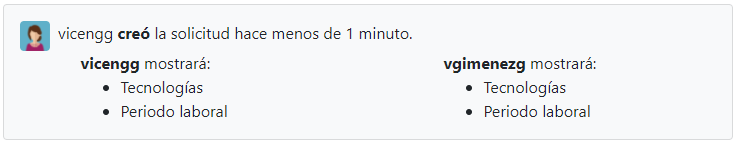
\includegraphics[width=15cm, keepaspectratio]{img/ActionDisplay.PNG}
        \caption{Ejemplo de componente web ActionDisplay.}\label{fig:component_action_display}
    \end{figure}

    Sus entradas son:

    \begin{itemize}
        \item \textbf{action:} Objeto con el contenido de la acción, ver definición de \emph{Action} en la Subsección~\ref{subsec:negotiation_value_objects}.
        \item \textbf{user:} Objeto que contiene la información del usuario en sesión, ver definición de \emph{User} en la Subsección~\ref{subsec:common_classes}.
        \item \textbf{isFirst:} Indica si el \emph{ActionDisplay} es o no el primer elemento de una lista, para su correcta visualización.
        \item \textbf{creator:} Objeto que contiene la información del usuario que creó la negociación, ver definición de \emph{User} en la Subsección~\ref{subsec:common_classes}.
        \item \textbf{receiver:} Objeto que contiene la información del usuario que inició la negociación, ver definición de \emph{User} en la Subsección~\ref{subsec:common_classes}.
    \end{itemize}

    \subsection{AppRouter}
    \label{subsec:wc_app_router}
    Este componente establece la relación de rutas entre las distintas vistas de la aplicación y permite navegar a algunas de ellas mediante una barra de navegación.
    Este componente se muestra en la Figura~\ref{fig:component_app_router}.

    \begin{figure}
        \centering
        
\includegraphics[width=15cm, keepaspectratio]{img/AppRouter.PNG}
        \caption{Componente web \emph{AppRouter}.}\label{fig:component_app_router}
    \end{figure}

    \subsection{Autocomplete}
    \label{subsec:wc_autocomplete}
    Este componente es una entrada de texto que ofrece al usuario una lista de sugerencias como ayuda para completar el texto que está ingresando.
    Los elementos aparecen filtrados según el texto que el usuario va escribiendo.
    Para ofrecer la lista de sugerencias este formulario realiza una petición HTTP a uno de los puntos de API definidos en la Subsección~\ref{subsec:reference_endpoints}.
    Este componente se muestra en la Figura~\ref{fig:component_autocomplete}.

    \begin{figure}
        \centering
        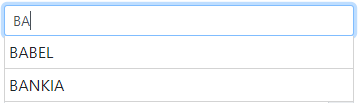
\includegraphics[width=10cm, keepaspectratio]{img/Autocomplete.PNG}
        \caption{Ejemplo de componente web \emph{Autocomplete}.}\label{fig:component_autocomplete}
    \end{figure}

    Sus entradas son:

    \begin{itemize}
        \item \textbf{url:} URL de datos de referencia a la que consulta el componente, ver Subsección~\ref{subsec:reference_endpoints}.
        \item \textbf{placeholder:} Texto opcional que se muestra en la entrada de texto cuando el usuario no ha escrito nada.
        \item \textbf{footer:} Texto opcional que se muestra como pie de la entrada de texto.
        \item \textbf{value:} Variable que contiene el texto ingresado en la entrada de texto.
        \item \textbf{onChange:} Función de tipo callback que se ejecuta cuando hay cambios en la entrada de texto.
        \item \textbf{onSelect:} Función de tipo callback que se ejecuta cuando el usuario selecciona una sugerencia.
        \item \textbf{onSubmit:} Función de tipo callback que se ejecuta cuando el usuario presiona la tecla \emph{introducir}.
        \item \textbf{styleClasses:} Clases adicionales de estilos que se pueden añadir al componente.
    \end{itemize}

    \subsection{AutocompleteMultiple}
    \label{subsec:wc_autocomplete_multiple}
    Este componente es una entrada de texto que ofrece al usuario una lista de sugerencias como ayuda para completar el texto que está ingresando,
    similar al componente descrito anteriormente en la Subsubsección~\ref{subsec:wc_autocomplete}, pero que de forma diferente a este permite seleccionar múltiples valores que se muestran a continuación de la entrada de texto.
    Los elementos aparecen filtrados según el texto que el usuario va escribiendo.
    Para ofrecer la lista de sugerencias este formulario realiza una petición HTTP a uno de los puntos de API definidos en la Subsección~\ref{subsec:reference_endpoints}.
    Este componente se muestra en la Figura~\ref{fig:component_autocomplete_multiple}.

    \begin{figure}
        \centering
        
\includegraphics[width=10cm, keepaspectratio]{img/AutocompleteMultiple.PNG}
        \caption{Ejemplo de componente web \emph{AutocompleteMultiple}.}\label{fig:component_autocomplete_multiple}
    \end{figure}

    Sus entradas son:

    \begin{itemize}
        \item \textbf{url:} URL de datos de referencia a la que consulta el componente, ver Subsección~\ref{subsec:reference_endpoints}.
        \item \textbf{placeholder:} Texto opcional que se muestra en la entrada de texto cuando el usuario no ha escrito nada.
        \item \textbf{footer:} Texto opcional que se muestra como pie de la entrada de texto.
        \item \textbf{values:} Variable que contiene las lista de valores ingresados en la entrada de texto.
        \item \textbf{setValues:} Función que establece el valor de la variable \emph{values}.
        \item \textbf{styleClasses:} Clases adicionales de estilos que se pueden añadir al componente.
    \end{itemize}

    \subsection{CardSkeleton}
    \label{subsec:wc_card_skeleton}
    Componente visual que muestra una tarjeta con datos en blanco, utilizado para mantener una experiencia de usuario agradable durante el tiempo que tardan en cargarse algunos que se consulta al API REST.
    Este componente se muestra en la Figura~\ref{fig:component_card_skeleton}.

    \begin{figure}
        \centering
        
\includegraphics[width=15cm, keepaspectratio]{img/CardSkeleton.PNG}
        \caption{Ejemplo de componente web \emph{CardSkeleton}.}\label{fig:component_card_skeleton}
    \end{figure}

    Sus entradas son:

    \begin{itemize}
        \item \textbf{lines:} Número de líneas en blanco que componen la tarjeta.
    \end{itemize}

    \subsection{Checkbox}
    \label{subsec:wc_checkbox}
    Este componente permite seleccionar un valor booleano para una variable mediante un elemento de tipo casilla de verificación, o un interruptor dependiendo del estilo que se elija.
    El componente se muestra en la Figura~\ref{fig:component_checkbox}.

    \begin{figure}
        \centering
        
\includegraphics[width=3cm, keepaspectratio]{img/Checkbox.PNG}
        \caption{Ejemplos de componentes web \emph{Checkbox}.}\label{fig:component_checkbox}
    \end{figure}

    Sus entradas son:

    \begin{itemize}
        \item \textbf{value:} Variable que contiene el valor de la casilla o interruptor.
        \item \textbf{setValue:} Función que establece el valor de la variable \emph{value} en los cambios de estado de la casilla o interruptor.
        \item \textbf{labelOff:} Texto que acompaña al elemento cuando está desmarcado.
        \item \textbf{labelOn:} Texto que acompaña al elemento cuando está marcado.
        \item \textbf{type:} Por defecto \emph{checkbox}, muestra una casilla de verificación si su valor es \emph{checkbox} o un interruptor si su valor es \emph{switch}.
        \item \textbf{disabled:} Si se estable su valor a \emph{true}, deshabilita el componente para que no sea modificable.
    \end{itemize}

    \subsection{Chip}
    \label{subsec:wc_chip}
    Componente de tipo visual que permite representar un texto envuelto en un óvalo. Se usa para reprensentar un elemento en un listado de valores.
    Este componente se muestra en la Figura~\ref{fig:component_chip}.

    \begin{figure}
        \centering
        
\includegraphics[width=12cm, keepaspectratio]{img/Chip.PNG}
        \caption{Ejemplo con varios componentes \emph{Chip} seguidos.}\label{fig:component_chip}
    \end{figure}

    Sus entradas son:

    \begin{itemize}
        \item \textbf{value:} Texto del elemento de tipo \emph{Chip}.
    \end{itemize}

    \subsection{ClosableChip}
    \label{subsec:wc_closable_chip}
    Componente de tipo visual que permite representar un texto envuelto en un óvalo, similar al componente Chip~\ref{subsec:wc_chip}, pero que a diferencia de este permite ser eliminado realizando click en un botón de aspa.
    Se usa para reprensentar un elemento eliminable en un listado de valores.
    Este componente se muestra en la Figura~\ref{fig:component_closable_chip}.

    \begin{figure}
        \centering
        
\includegraphics[width=11cm, keepaspectratio]{img/ClosableChip.PNG}
        \caption{Ejemplo con varios componentes \emph{ClosableChip} seguidos.}\label{fig:component_closable_chip}
    \end{figure}

    Sus entradas son:

    \begin{itemize}
        \item \textbf{value:} Texto del elemento de tipo \emph{Chip}.
        \item \textbf{onClose:} Función que se ejecuta cuando se realiza click en el botón de aspa.
    \end{itemize}

    \subsection{DateInput}
    \label{subsec:wc_date_input}
    Este componente es una entrada de texto que permite al usuario ingresar fechas.
    Este componente se muestra en la Figura~\ref{fig:component_date_input}.

    \begin{figure}
        \centering
        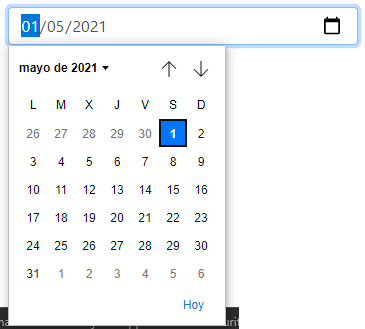
\includegraphics[width=7cm, keepaspectratio]{img/DateInput.PNG}
        \caption{Ejemplo de componente web \emph{DateInput}.}\label{fig:component_date_input}
    \end{figure}

    Sus entradas son:

    \begin{itemize}
        \item \textbf{footer:} Texto opcional que se muestra como pie de la entrada de texto.
        \item \textbf{value:} Variable que contiene el texto ingresado en la entrada de texto.
        \item \textbf{onChange:} Función de tipo callback que se ejecuta cuando hay cambios en la entrada de texto.
        \item \textbf{disabled:} Si se establece a \emph{true}, la entrada de texto permanece deshabilitada para que no sea modificable.
        \item \textbf{styleClasses:} Clases adicionales de estilos que se pueden añadir al componente.
    \end{itemize}

    \subsection{Modal}
    \label{subsec:wc_modal}
    Este componente web es una ventana modal que emerge en la página.
    Se utiliza para destacar operaciones que requieren atención especial por parte del usuario en el contexto de una vista.
    Este componente se muestra en la Figura~\ref{fig:component_modal}.

    \begin{figure}
        \centering
        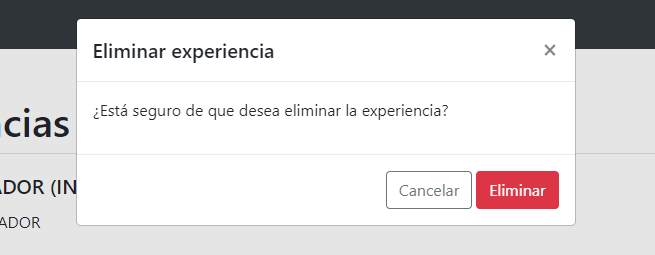
\includegraphics[width=10cm, keepaspectratio]{img/Modal.PNG}
        \caption{Ejemplo de componente web \emph{Modal}.}\label{fig:component_modal}
    \end{figure}

    Sus entradas son:

    \begin{itemize}
        \item \textbf{title:} Título de modal.
        \item \textbf{children:} Una lista de dos elementos HTML (o componentes web) que el modal puede mostrar como contenido, el primero en el cuerpo del modal y el segundo en el pie del modal.
        \item \textbf{isShown:} Variable que controla si el modal se muestra o no.
        \item \textbf{close:} Función que maneja el cierre del modal.
        \item \textbf{additionalClasses:} Clases adicionales de estilos que se pueden añadir al componente.
    \end{itemize}

    \subsection{MoneyInput}
    \label{subsec:wc_money_input}
    Este componente es una entrada de texto que permite al usuario ingresar cantidades de dinero.
    Este componente se muestra en la Figura~\ref{fig:component_money_input}.

    \begin{figure}
        \centering
        
\includegraphics[width=7cm, keepaspectratio]{img/MoneyInput.PNG}
        \caption{Ejemplo de componente web \emph{MoneyInput}.}\label{fig:component_money_input}
    \end{figure}

    Sus entradas son:

    \begin{itemize}
        \item \textbf{placeholder:} Texto opcional que se muestra en la entrada de texto cuando el usuario no ha escrito nada.
        \item \textbf{footer:} Texto opcional que se muestra como pie de la entrada de texto.
        \item \textbf{value:} Variable que contiene el dinero ingresado en la entrada de texto.
        \item \textbf{onChange:} Función de tipo callback que se ejecuzta cuando hay cambios en la entrada de texto.
        \item \textbf{currency:} Código ISO de la moneda en la cual se introduce la cantidad.
        \item \textbf{styleClasses:} Clases adicionales de estilos que se pueden añadir al componente.
    \end{itemize}

    \subsection{NavbarUser}
    \label{subsec:wc_navbar_user}
    Este componentemuestra el usuario que está en sesión en la barra superior de navegación.
    Además le permite cerrar sesión mediante un botón desplegable.
    Este componente consulta directamente al punto de API de obtención de usuario para recuperar los datos del usuario en sesión. Ver~\ref{subsec:get_user}.
    Este componente se muestra en la Figura~\ref{fig:component_navbar_user}

    \begin{figure}
        \centering
        
\includegraphics[width=6cm, keepaspectratio]{img/NavbarUser.PNG}
        \caption{Ejemplo de componente web \emph{NavbarUser}.}\label{fig:component_navbar_user}
    \end{figure}

    \subsection{NegotiableWorkExperience}
    \label{subsec:wc_negotiable_work_experience}
    Este componente de tipo tarjeta permite operar sobre los campos de una experiencia laboral, modificando la visibilidad de los campos de cara a realizar una oferta o solicitud de información.
    Cada uno de los campos privados de la experiencia laboral posee su propio interruptor que controla la visibilidad, el usuario elije si quiere mantener un campo privado o ofrecerlo/pedirlo como público.
    Este componente se muestra en la Figura~\ref{fig:component_negotiable_work_experience}.

    \begin{figure}
        \centering
        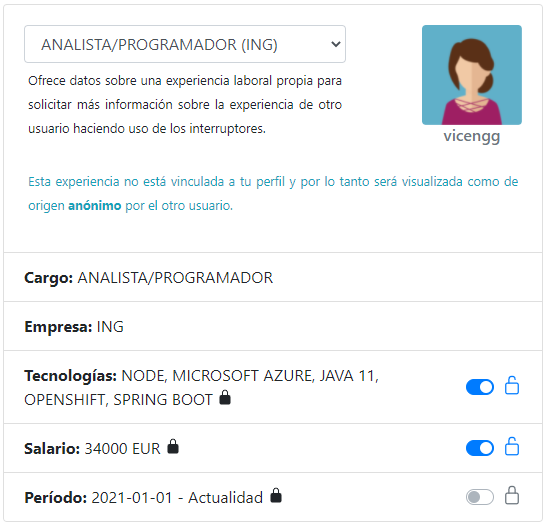
\includegraphics[width=10cm, keepaspectratio]{img/NegotiableWorkExperience.PNG}
        \caption{Ejemplo de componente web \emph{NegotiableWorkExperience}.}\label{fig:component_negotiable_work_experience}
    \end{figure}

    Sus entradas son:

    \begin{itemize}
        \item \textbf{workExperience:} Objeto con el contenido de la experiencia laboral sobre la que se va a hacer el ofrecimiento/solicitud de visibilidad, ver definición de \emph{WorkExperienceEntity} en la Subsección~\ref{subsec:work_experience_entity}.
        \item \textbf{children:} Lista de tres elementos HTML. La tarjeta puede contener hasta tres elementos HTML (o componentes web) en su cuerpo. Los dos primeros representados a la izquierda del avatar del usuario y el último justo debajo.
        \item \textbf{visibilityRequest:} Variable que contiene la información de la visibilidad de la experiencia laboral que se está manipulando en el componente, ver definición de \emph{VisibilityRequest} en la Subsección~\ref{subsec:negotiation_value_objects}.
        \item \textbf{setVisibilityRequest:} Función que establece el valor de la variable \emph{visibilityRequest}.
        \item \textbf{disabled:} Si se establece a \emph{true} deshabilita el componente para evitar su modificación.
    \end{itemize}

    \subsection{NegotiationSummary}
    \label{subsec:wc_negotiation_summary}
    Este componente de tipo tarjeta muestra de forma resumida el último estado de una negociación, es decir, si está pendiente, aceptada o cancelada, los datos que los usuarios ofrecen y solicitan y los usuarios que intervienen en ella.
    Este componente se muestra en la Figura~\ref{fig:component_negotiation_summary}.

    \begin{figure}
        \centering
        
\includegraphics[width=15cm, keepaspectratio]{img/NegotiationSummary.PNG}
        \caption{Ejemplo de componente web \emph{NegotiationSummary}.}\label{fig:component_negotiation_summary}
    \end{figure}

    Sus entradas son:

    \begin{itemize}
        \item \textbf{negotiation:} Objeto con el contenido de la negociación de la cual se está mostrando el resumen, ver definición de \emph{NegotiationEntity} en la Subsección~\ref{subsec:negotiation_entity}.
        \item \textbf{user:} Objeto que contiene la información del usuario en sesión, ver definición de \emph{User} en la Subsección~\ref{subsec:common_classes}.
    \end{itemize}

    \subsection{OwnWorkExperience}
    \label{subsec:wc_own_work_experience}
    Este componente de tipo tarjeta muestra de forma resumida el contenido de una experiencia laboral del usuario en sesión, así como la visibilidad de los campos. Además permite al usuario eliminar su experiencia laboral y navegar a la vista de edición de experiencias laborales.
    Este componente se muestra en la Figura~\ref{fig:component_own_work_experience}.

    \begin{figure}
        \centering
        
\includegraphics[width=15cm, keepaspectratio]{img/OwnWorkExperience.PNG}
        \caption{Ejemplo de componente web \emph{OwnWorkExperience}.}\label{fig:component_own_work_experience}
    \end{figure}

    Sus entradas son:

    \begin{itemize}
        \item \textbf{workExperience:} Objeto con el contenido de la experiencia laboral de la que se muestran los datos, ver definición de \emph{WorkExperienceEntity} en la Subsección~\ref{subsec:work_experience_entity}.
        \item \textbf{afterDelete:} Función de tipo callback que se ejecuta después del borrado de la experiencia laboral.
        \item \textbf{editable:} Si se establece a \emph{true} permite eliminar y navegar a la vista de modifiación de la experiencia laboral.
    \end{itemize}

    \subsection{Radio}
    \label{subsec:wc_radio}
    Este componente contiene una serie de botones de radio que permiten elegir entre varias opciones para establecer una variable.
    Este componente se muestra en la Figura~\ref{fig:component_radio}.

    \begin{figure}
        \centering
        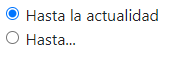
\includegraphics[width=5cm, keepaspectratio]{img/Radio.PNG}
        \caption{Ejemplo de componente web \emph{Radio}.}\label{fig:component_radio}
    \end{figure}

    Sus entradas son:

    \begin{itemize}
        \item \textbf{options:} Un objeto de tipo JSON que alimenta de opciones al componente. Cada clave representa el identificador de una posible opción, mientras que cada valor representa el texto que se mostrará para esta opción por pantalla.
        \item \textbf{selected:} Variable que contiene la opción seleccionada.
        \item \textbf{changeOption:} Función de tipo callback que se ejecuta cuando la opción del componente cambia.
    \end{itemize}

    \subsection{RequestButton}
    \label{subsec:wc_request_button}
    Este componente de tipo botón dispara peticiones HTTP cuando se hace click en él.
    Este componente se muestra en la Figura~\ref{fig:component_request_button}.

    \begin{figure}
        \centering
        
\includegraphics[width=5cm, keepaspectratio]{img/RequestButton.PNG}
        \caption{Ejemplo de componente web \emph{RequestButton}.}\label{fig:component_request_button}
    \end{figure}

    Sus entradas son:

    \begin{itemize}
        \item \textbf{text:} Texto del botón.
        \item \textbf{url:} URL a la que realizará las llamadas HTTP.
        \item \textbf{method:} Método HTTP, por defecto \emph{GET}.
        \item \textbf{body:} Cuerpo de la solicitud HTTP, por defecto vacío.
        \item \textbf{headers:} Cabeceras de la solicitud HTTP, por defecto incluye la cabecera \emph{Content-Type: application/json}.
        \item \textbf{styleClasses:} Clases de estilo adicionales que se le pueden añadir al botón.
        \item \textbf{onSucces:} Función de tipo callback que se ejecuta cuando la petición ha terminado y permite manejar la respuesta.
    \end{itemize}

    \subsection{Select}
    \label{subsec:wc_select}
    Este componente genera un elemento de tipo seleccionable que permite elegir entre varias opciones en un menú desplegable.
    Este componente se muestra en la Figura~\ref{fig:component_select}.

    \begin{figure}
        \centering
        
\includegraphics[width=10cm, keepaspectratio]{img/Select.PNG}
        \caption{Ejemplo de componente web \emph{Select}.}\label{fig:component_select}
    \end{figure}

    Sus entradas son:

    \begin{itemize}
        \item \textbf{values:} Un objeto de tipo JSON que alimenta de opciones al componente. Cada clave representa el identificador de una posible opción, mientras que cada valor representa el texto que se mostrará en el desplegable para esa opción.
        \item \textbf{onChange:} Función de tipo callback que se ejecuta cuando hay cambios en el seleccionable.
        \item \textbf{styleClasses:} Clases adicionales de estilos que se pueden añadir al componente.
    \end{itemize}

    \subsection{WorkExperience}
    \label{subsec:wc_work_experience}
    Este componente de tipo tarjeta muestra de forma resumida el contenido de una experiencia laboral resultado de una búsqueda.
    Este componente se muestra en la Figura~\ref{fig:component_work_experience}.

    \begin{figure}
        \centering
        
\includegraphics[width=15cm, keepaspectratio]{img/WorkExperience.PNG}
        \caption{Ejemplo de componente web \emph{WorkExperience}.}\label{fig:component_work_experience}
    \end{figure}

    Sus entradas son:
    \begin{itemize}
        \item \textbf{workExperience:} Objeto con el contenido de la experiencia laboral de la que se muestran los datos, ver definición de \emph{WorkExperienceEntity} en la Subsección~\ref{subsec:work_experience_entity}.
        \item \textbf{editable:} Si se establece a \emph{true} habilita un botón que permite navegar a la vista de negociación.
    \end{itemize}

    \subsection{WorkExperienceSummary}
    \label{subsec:wc_work_experience_summary}
    Este componente de tipo tarjeta muestra de forma resumida el contenido de una experiencia laboral vinculada a una negociación en la vista de detalles de negociación.
    El componente se muestra en la Figura~\ref{fig:component_work_experience_summary}.
    \begin{figure}
        \centering
        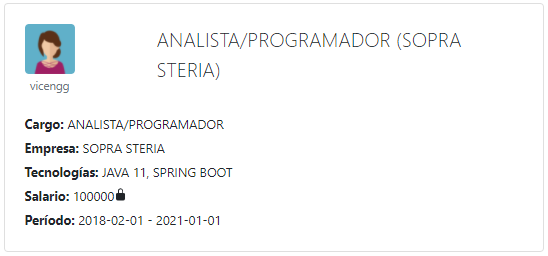
\includegraphics[width=10cm, keepaspectratio]{img/WorkExperienceSummary.PNG}
        \caption{Ejemplo de componente web \emph{WorkExperienceSummary}.}\label{fig:component_work_experience_summary}
    \end{figure}

    Sus entradas son:

    \begin{itemize}
        \item \textbf{workExperience:} Objeto con el contenido de la experiencia laboral de la que se muestran los datos, ver definición de \emph{WorkExperienceEntity} en la Subsección~\ref{subsec:work_experience_entity}.
        \item        \textbf{visibilityRequest:} Variable que contiene la información de la visibilidad de la experiencia laboral de la que se muestran los datos, ver definición de \emph{VisibilityRequest} en la Subsección~\ref{subsec:negotiation_value_objects}.
        \item \textbf{setVisibilityRequest:} Función que establece el valor de la variable \emph{visibilityRequest}.
    \end{itemize}


    \section{Vistas}
    \label{sec:views}
    En esta sección se describen las vistas que componen la aplicación web.
    Para crear el sistema de vistas de la aplicación de una sola pagína, el enrutador de React asocia a cada vista una ruta de navegador concreta. Esta es la relación entre vistas y rutas dentro de la aplicación:

    \begin{itemize}
        \item Vista de \emph{Mis experiencias}: Asociada a la ruta \emph{/my-work-experiences}.
        \item Vista de \emph{Crear experiencia}: Asociada a la ruta \emph{/add-work-experience}.
        \item Vista de \emph{Editar experiencia}: Asociada a la ruta \emph{/modify-work-experience/\{workExperienceId\}}, donde \emph{workExperienceId} es el identificador único de la experiencia a editar.
        \item Vista de \emph{Buscar experiencias}: Asociada a la ruta \emph{/search-work-experiences}.
        \item Vista de \emph{Solicitud de información}: Asociada a la ruta \emph{/create-information-request/\{workExperienceId\}},
        donde \emph{workExperienceId} es el identificador único de la experiencia sobre la que se quiere solicitar información.
        \item Vista de \emph{Mis solicitudes}: Asociada a la ruta \emph{/my-negotiations}.
        \item Vista de \emph{Detalles de solicitud}: Asociada a la ruta \emph{/negotiation-details/\{negotiationId\}},
        donde \emph{negotiationId} es el identificador único de la negociación de la que se consultan los detalles.
    \end{itemize}

    Como apoyo a la sección se incluye el diagrama de la Figura~\ref{fig:navegation_diagram} que representa de forma esquemática la navegabilidad entre las distintas vistas.

    \begin{figure}
        \centering
        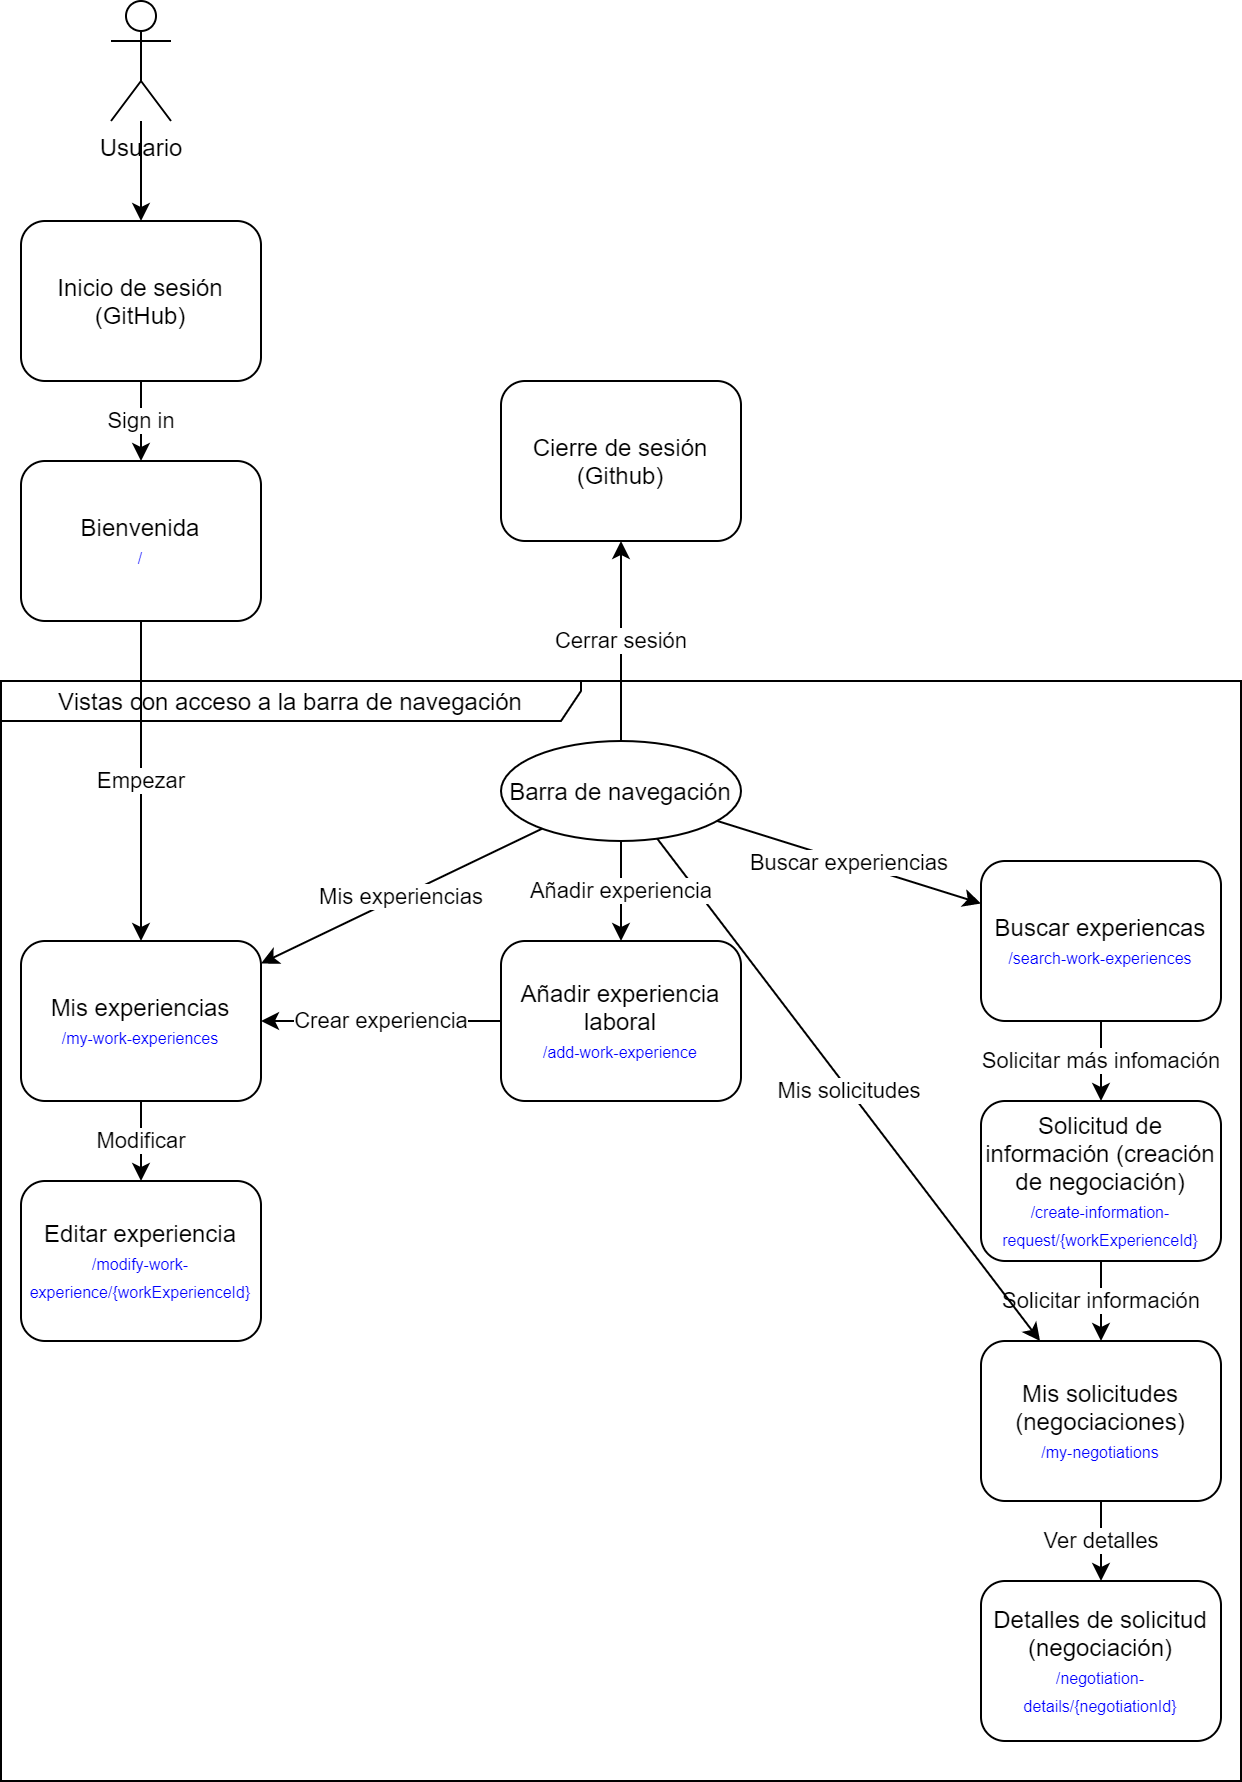
\includegraphics[width=10cm, keepaspectratio]{img/Navegacion.png}
        \caption{Diagrama de navegación entre las vistas de la aplicación.}\label{fig:navegation_diagram}
    \end{figure}

    \subsection{Inicio de sesión}
    \label{subsec:view_sign_in}
    Esta vista es externa a la aplicación y es provista por GitHub.
    Su propósito es permitir que los usuarios inicien sesión con su cuenta de GitHub.
    Por lo tanto aquellos usuarios que traten de acceder a la \emph{Vista de bienvenida} de la aplicación sin haber iniciado sesión previamente en GitHub serán redirigidos a esta vista.
    Una vez se introducen un usuario y clave de GitHub válido y se hace click en el botón \emph{Sign in} que se muestra en la Figura~\ref{fig:view_sign_in} el usuario es conducido a la \emph{Vista de bienvenida}.

    \begin{figure}
        \centering
        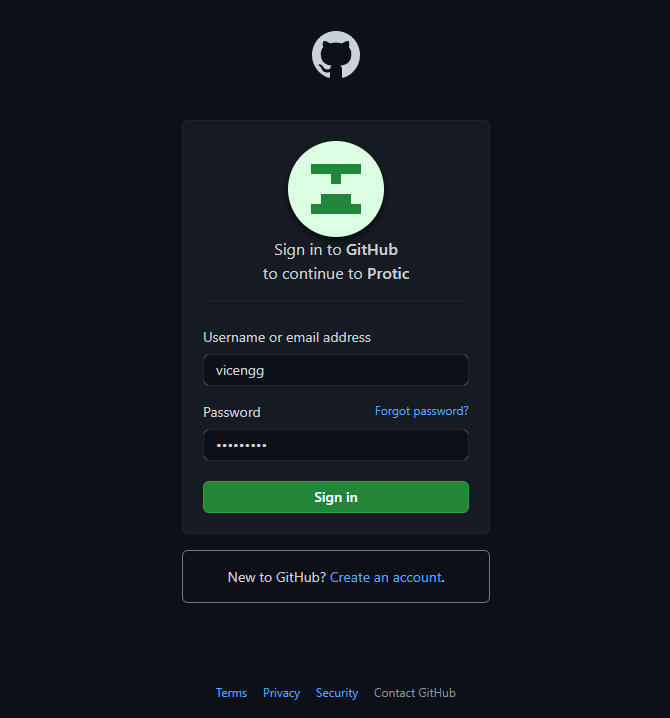
\includegraphics[width=15cm, keepaspectratio]{img/login.PNG}
        \caption{Vista de inicio de sesión.}\label{fig:view_sign_in}
    \end{figure}

    \subsection{Bienvenida}
    \label{subsec:view_welcome}
    Es la primera vista de la aplicación, sirve como punto de entrada al resto de vistas.
    En ella el usuario ve su propio perfil de GitHub en sesión y puede leer una breve descripción de la herramienta.
    Una vez el usuario hace click en el botón \emph{Empezar} que se muestra en la Figura~\ref{fig:view_welcome} este es redirigido a la vista de \emph{Mis experiencias}.

    \begin{figure}
        \centering
        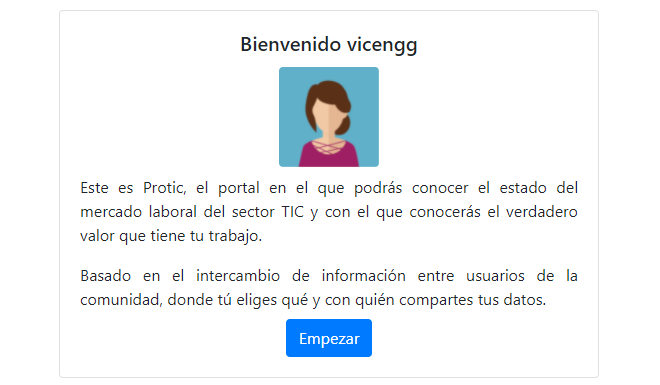
\includegraphics[width=15cm, keepaspectratio]{img/welcome.PNG}
        \caption{Vista de bienvenida.}\label{fig:view_welcome}
    \end{figure}

    \subsection{Mis experiencias}
    \label{subsec:view_my_work_experiences}
    El propósito de esta vista es mostrar a cada usuario una lista con sus propias experiencias laborales,
    así como permitirle borrarlas o editarlas (redirigiéndole en este último caso a la vista de \emph{Editar mi experiencia}.
    La primera vez que un usuario ingrese en la aplicación, al no poseer ninguna experiencia añadida verá esta vista como la que se muestra en la Figura~\ref{fig:view_my_work_experiences_empty}, desde donde podrá navegar a la vista de \emph{Añadir experiencia}.
    Los usuarios que ya tengan experiencias laborales guardadas en la aplicación, verán esta vista como la que se muestra en la Figura~\ref{fig:view_my_work_experiences}. Desde aquí podrán eliminar cada una de sus experiencias haciendo click en el botón \emph{Eliminar} y confirmando la operación en el modal emergente.
    También para cada experiencia, será redireccionado a la vista \emph{Editar experiencia} haciendo click en el botón \emph{Editar}.

    \begin{figure}
        \centering
        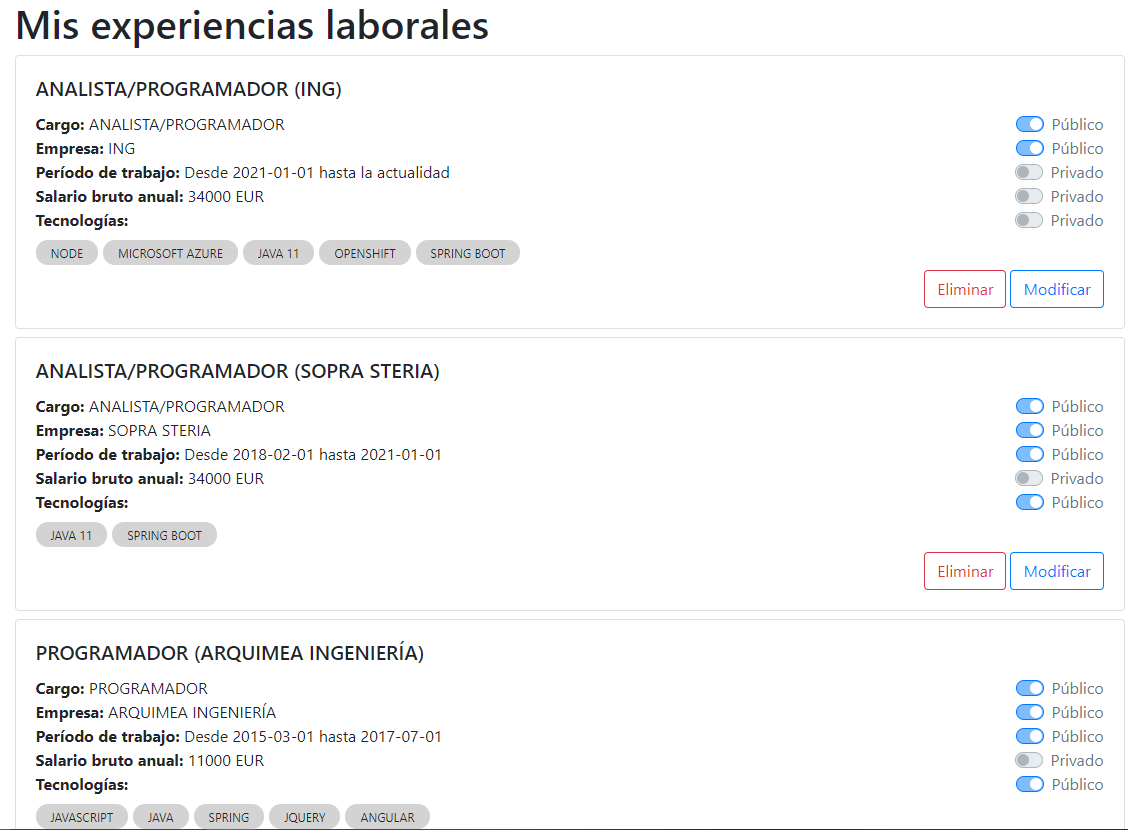
\includegraphics[width=15cm, keepaspectratio]{img/my_we.PNG}
        \caption{Vista \emph{Mis experiencias}.}\label{fig:view_my_work_experiences}
    \end{figure}

    \begin{figure}
        \centering
        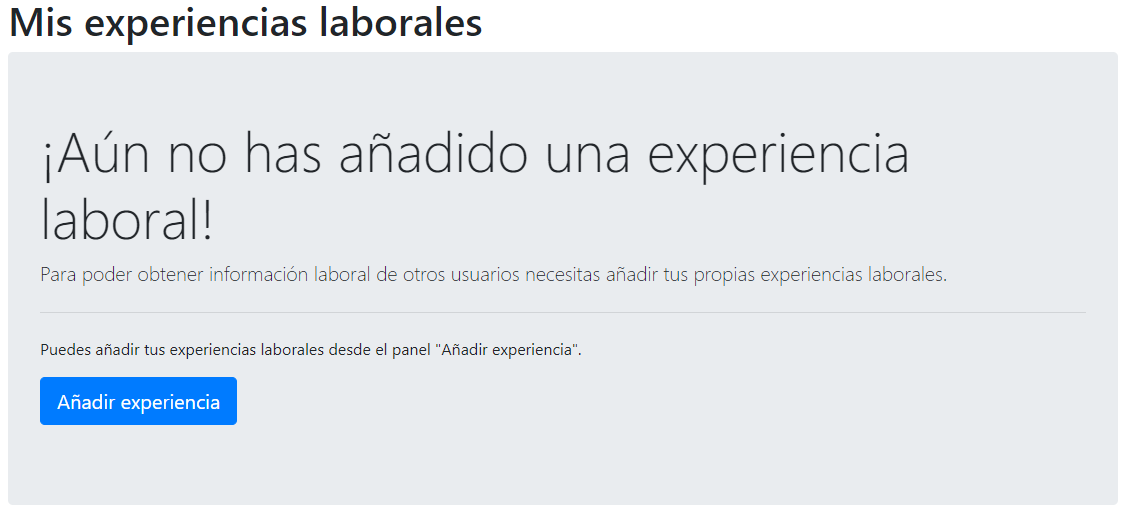
\includegraphics[width=15cm, keepaspectratio]{img/my_we_empty.PNG}
        \caption{Vista \emph{Mis experiencias} vacía.}\label{fig:view_my_work_experiences_empty}
    \end{figure}

    \paragraph{Barra de navegación}
    En adelante, todas las vistas de la aplicación tendrán acceso a la barra de navegación (ver Subsección~\ref{subsec:wc_app_router}), que permite navegar desde cualquier punto a:
    \begin{itemize}
        \item La vista de \emph{Añadir experiencia}.
        \item La vista de \emph{Mis experiencias}.
        \item La vista de \emph{Buscar experiencia}.
        \item La vista de \emph{Mis solicitudes}.
        \item La vista de \emph{Cierre de sesión} de GitHub, invalidando previamente la sesión en la aplicación.
    \end{itemize}

    \subsection{Añadir experiencia}
    \label{subsec:view_add_work_experience}
    Esta vista proporciona un formulario que permite al usuario crear una nueva experiencia laboral.
    Este formulario está compuesto por cinco campos como se muestra en la figura Figura~\ref{fig:view_add_work_experience}:
    \begin{itemize}
        \item Puesto de trabajo: Nombre del puesto de trabajo de la experiencia laboral.
        \item Empresa: Nombre de la empresa de la experiencia laboral.
        \item Tecnologías: Listado de las tecnologías que se emplearon en la experienca laboral.
        \item Salario: Salario bruto anual que se percibió en la experiencia laboral.
        \item Periodo laboral: Compuesto de una entrada de texto para la fecha de inicio, un botón de radio que permite indicar si la experiencia dura hasta el presente, y en caso negativo, otra entrada de texto para la fecha de fin.
    \end{itemize}
    Además cada campo tiene un interruptor que permite elegir si el campo tiene una visibilidad pública o privada para el resto de usuarios. Aquellos campos marcados como privados solo serán visibles para el propio usuario y para aquellos que hayan finalizado una negociación con el con el resultado de revelar dicho campo.
    Finalmente el formulario pregunta al usuario si desea vincular la experiencia que está creando con su perfil, en caso negativo esta experiencia aparecerá como anónima para el resto de usuarios.
    Una vez el usuario hace click en el botón \emph{Crear experiencia laboral}, la experiencia será creada y el usario redirigido a la vista \emph{Mis experiencias}.

    \begin{figure}
        \centering
        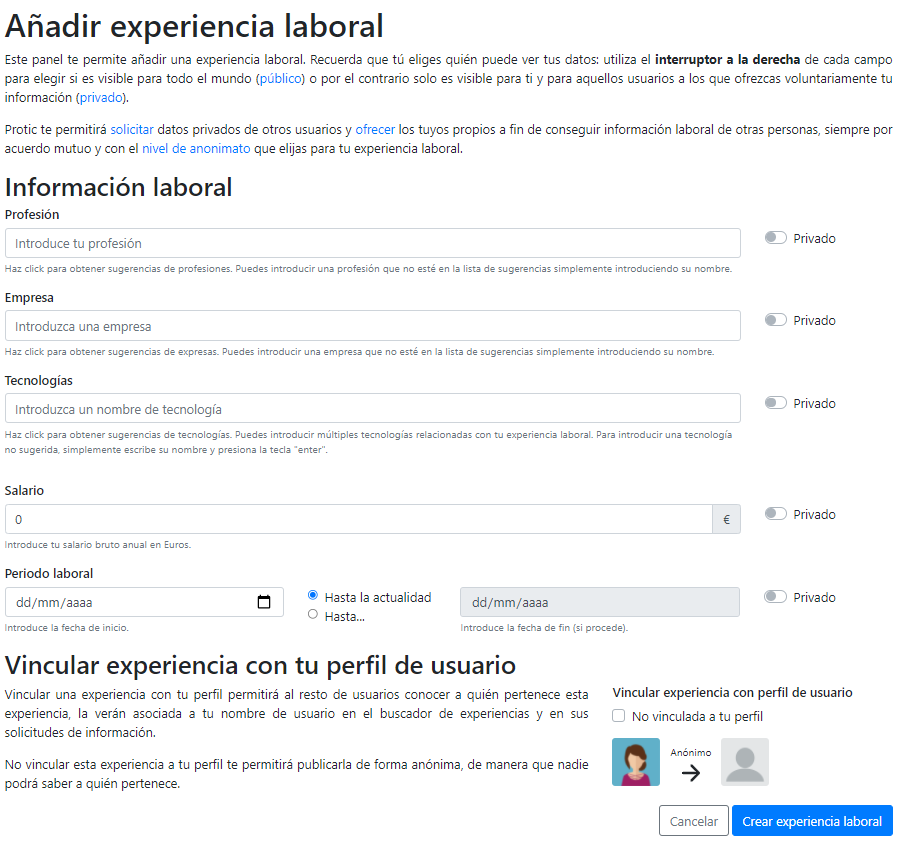
\includegraphics[width=15cm, keepaspectratio]{img/create_we.PNG}
        \caption{Vista \emph{Añadir experiencia}.}\label{fig:view_add_work_experience}
    \end{figure}

    \subsection{Editar experiencia}
    \label{subsec:view_edit_work_experience}
    El propósito de esta vista es permitir a un usuario modificar datos de una de sus experiencias laborales.
    Esta vista proporciona un formulario igual que el de la vista \emph{Añadir experiencia}, pero con los campos ya cumplimentados con la información de la experiencia laboral a editar para que el usuario los modifique.
    La vista está representada en la Figura~\ref{fig:view_edit_work_experience}.
    Una vez el usuario hace click en el botón \emph{Guardar}, la experiencia será modificada y el usario redirigido a la vista \emph{Mis experiencias}.

    \begin{figure}
        \centering
        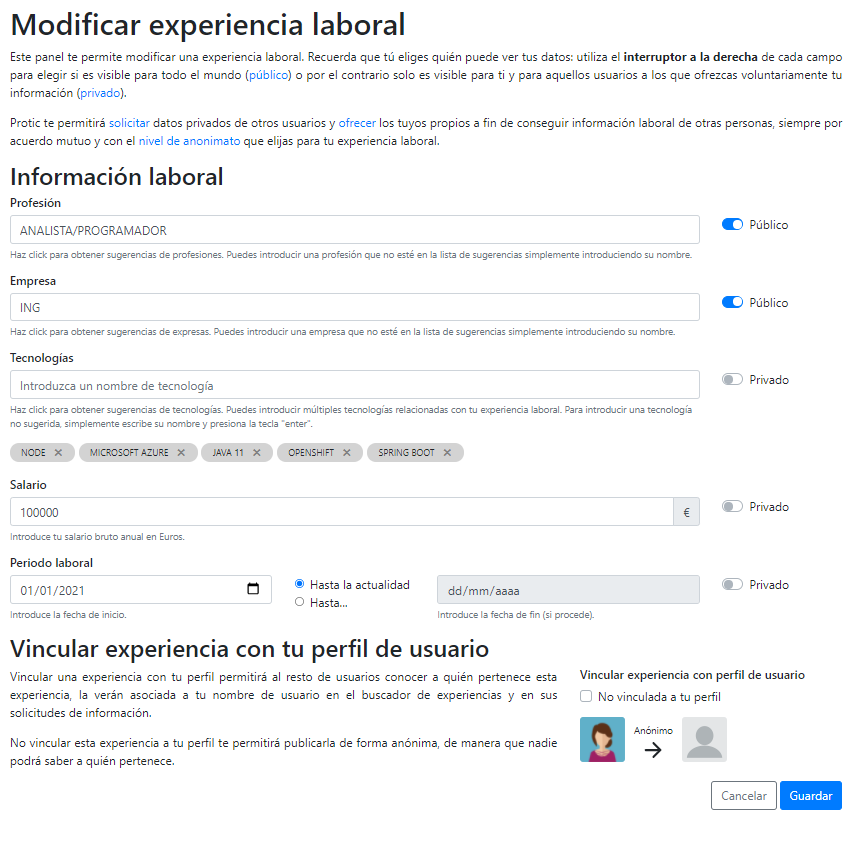
\includegraphics[width=15cm, keepaspectratio]{img/edit_we.PNG}
        \caption{Vista \emph{Editar experiencia}.}\label{fig:view_edit_work_experience}
    \end{figure}

    \subsection{Buscar experiencias}
    \label{subsec:view_search_work_experiences}
    Esta vista sirve al usuario para buscar experiencias laborales de otros usuarios.
    Para ello posee una serie de filtros en la parte superior como se muestra en la Figura~\ref{fig:view_search_work_experiences}:

    \begin{itemize}
        \item Puesto de trabajo: Filtra aquellas experiencias cuyo puesto de trabajo es un campo público y contiene la cadena de texto escrita en la entrada de texto.
        \item Empresa: Filtra aquellas experiencias cuya expresa es un campo público y contiene la cadena de texto escrita en la entrada de texto.
        \item Tecnologías: Filtra aquellas experiencias que contienen las tecnologías especificadas en el filtro.
        \item Salario mínimo: Filtra aquellas experiencias que tengan un salario superior al especificado.
        \item Salario máximo: Filtra aquellas experiencias que tengan un salario inferior al especificado.
        \item Fecha de entrada mínima: Filtra aquellas experiencias cuya fecha de entrada sea posterior a la especificada.
        \item Fecha de entrada máxima: Filtra aquellas experiencias cuya fecha de entrada sea anterior a la especificada.
    \end{itemize}

    Las experiencias que sean resultado de la búsqueda se presentaran en la vista como tarjetas (ver Subsección~\ref{subsec:wc_work_experience}).
    Cada experiencia con campos privados presentará un botón \emph{Solicitar más información} que permite navegar a la vista de \emph{Solicitud de información}.


    \begin{figure}
        \centering
        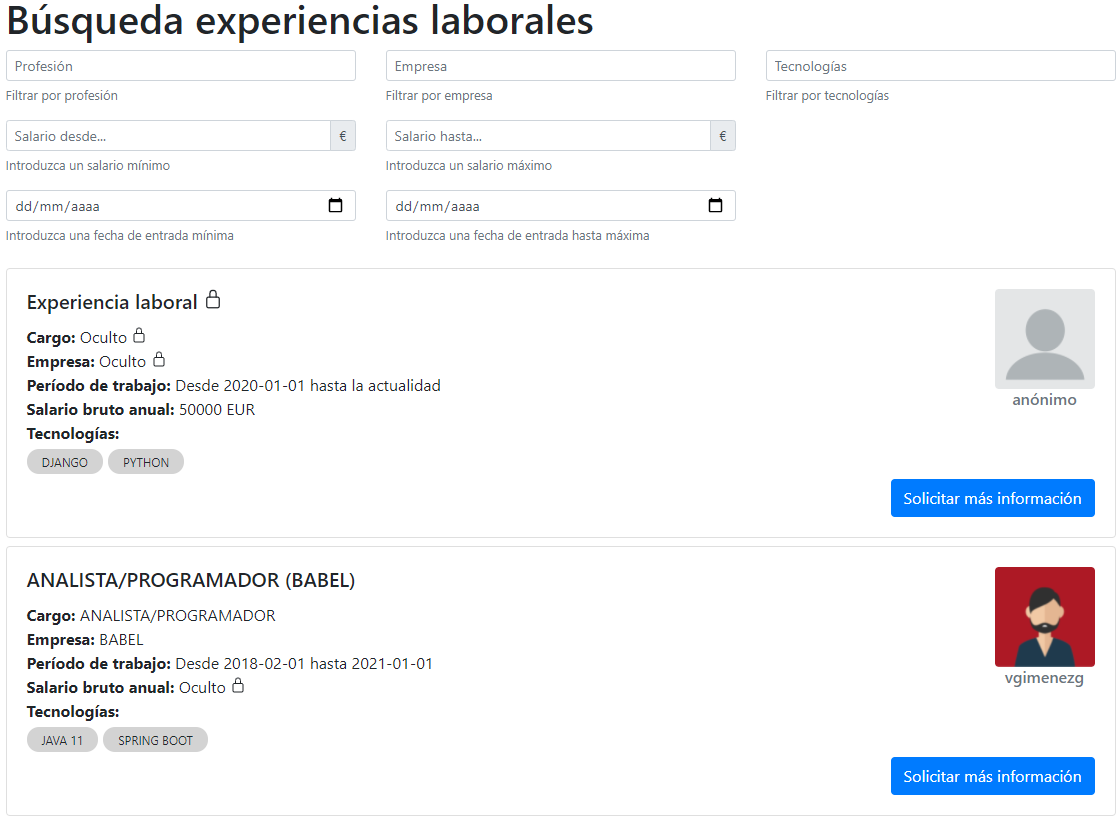
\includegraphics[width=15cm, keepaspectratio]{img/search_we.PNG}
        \caption{Vista \emph{Buscar experiencias}.}\label{fig:view_search_work_experiences}
    \end{figure}

    \subsection{Solicitud de información}
    \label{subsec:view_create_negotiation}
    En esta vista, un usuario puede solicitar datos privados de una experiencia laboral de otro usuario, ofreciendo a la vez datos privados de una de sus experiencias laborales.
    Por ello la vista se divide en dos partes, como se muestra en la Figura~\ref{fig:view_create_negotiation}:

    \begin{itemize}
        \item Experiencia ofrecida: En la parte izquierda de la vista, el usuario solicitante puede elegir una de sus propias experiencias laborales en un seleccionador,
        y marcar aquellos campos que está dispuesto a revelar al usuario receptor de la solicitud.
        \item Experiencia solicitada: En la parte derecha de la vista, el usuario solicitante selecciona aquellos campos privados de la experiencia laboral del receptor que quiere que le sean revelados.
    \end{itemize}

    Una vez el usuario hace click en el botón \emph{Solicitar información} será redigirigido a la vista \emph{Mis solicitudes}.

    \begin{figure}
        \centering
        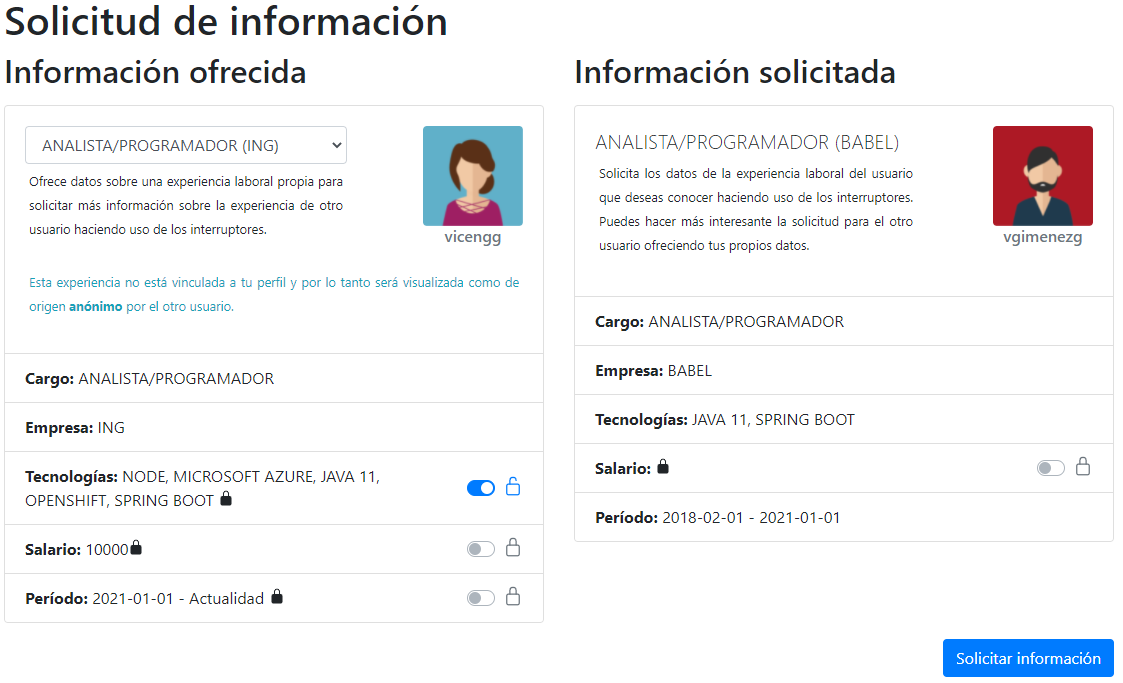
\includegraphics[width=15cm, keepaspectratio]{img/negotiate_we.PNG}
        \caption{Vista \emph{Solicitud de información}.}\label{fig:view_create_negotiation}
    \end{figure}

    \subsection{Mis solicitudes}
    \label{subsec:view_my_negotiations}
    Esta vista presenta la lista de negociaciones en las que el participa el usuario, ya sea porque ha creado solicitudes de información sobre experiencias de usuarios o bien porque otros usuarios han solicitado información de sus experiencias.
    Los usuarios que aun no participan en ninguna solicitud de información verán la vista como se muestra en la Figura~\ref{fig:view_my_negotiations_empty}.
    El resto de usuario verá una lista de tarjetas como la que se muestra en la figura Figura~\ref{fig:view_my_negotiations}.
    Cada tarjeta presentada en la lista corresponde con una solicitud de información, en ella aparece el solicitante en el lado izquierdo de la tarjeta, el receptor de la solicitud en el lado derecho, el estado de la negociación en el centro de la tarjeta, y un resumen del último paso de la solicitud en la parte de abajo.
    Haciendo click en el botón \emph{Ver detalles} de una tarjeta el usario navegará a la vista de \emph{Detalles de solicitud}.

    \begin{figure}
        \centering
        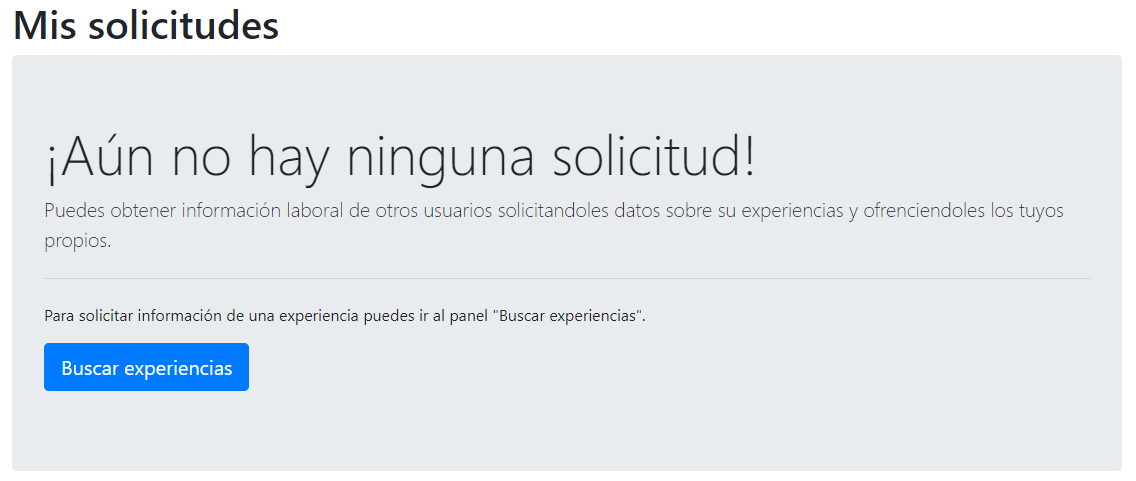
\includegraphics[width=15cm, keepaspectratio]{img/my_negotiations_empty.PNG}
        \caption{Vista \emph{Mis solicitudes} vacía.}\label{fig:view_my_negotiations_empty}
    \end{figure}

    \begin{figure}
        \centering
        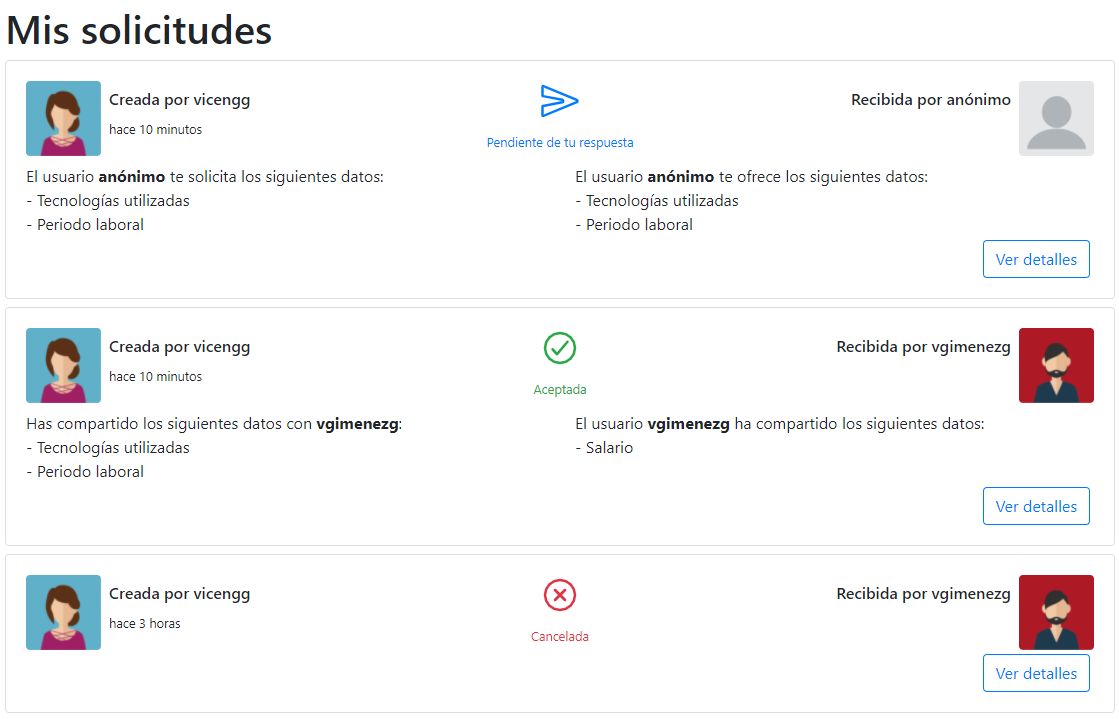
\includegraphics[width=15cm, keepaspectratio]{img/my_negotiations.PNG}
        \caption{Vista \emph{Mis solicitudes}.}\label{fig:view_my_negotiations}
    \end{figure}

    \subsection{Detalles de solictud}
    \label{subsec:view_negotiation_details}
    En esta vista se presentan al usuario los detalles de una solicitud.
    La vista se divide entres alturas:

    \begin{itemize}
        \item Parte superior: A la izquiera se muestran el estado de la solictud y el tiempo transcurrido desde que fue creada.
        A la derecha se muestran los botones con las posibles acciones que el usuario puede aplicar a la solicitud,
        como se muestra en la Figura~\ref{fig:negotiation_details_buttons}, a distinguir:
        \begin{itemize}
            \item Cancelar: Cancela la solicitud, cualquier usuario implicado en una solicitud pendiente tiene esta opción.
            \item Aceptar: En la negociación por turnos, cuando es el turno de un usuario este puede aceptar la solicitud.
            Esto implica que se revelará la información ofrecida y solicitada en el último turno a ambos usuarios implicados.
            \item Negociar: Cuando es el turno de un usuario, este puede negociar la solicitud para cambiar las condiciones impuestas
            por el otro usuario, es decir, el usuario puede modificar la visibilidad que se ofrece
            y solicita para los campos de las experiencias laborales asociadas a la solicitud.
            Hacer click en el botón de negociar hace que emerja un componente de tipo modal como el que se muestra en
            la Figura~\ref{fig:negotiation_details_modal}, similar a la vista de \emph{Solcitud de información}.
            Cuando el usuario hace click en el botón \emph{Enviar} del modal, se genera un nuevo paso en la solicitud,
            y el turno pasa al otro usuario implicado
        \end{itemize}
        \item Parte media: A la izquiera se muestra una tarjeta con los detalles de la experiencia laboral ofrecida en la solicitud.
        A la derecha otra tarjeta con los detalles de la experiencia laboral solicitada.
        \item Parte inferior: A modo de conversación aparecen los distintos pasos que los usuarios
        implicados han ido dando en la negociación desde su creación hasta su estado actual, como se muestra en la Figura~\ref{fig:negotiation_details}.
    \end{itemize}


    \begin{figure}
        \centering
        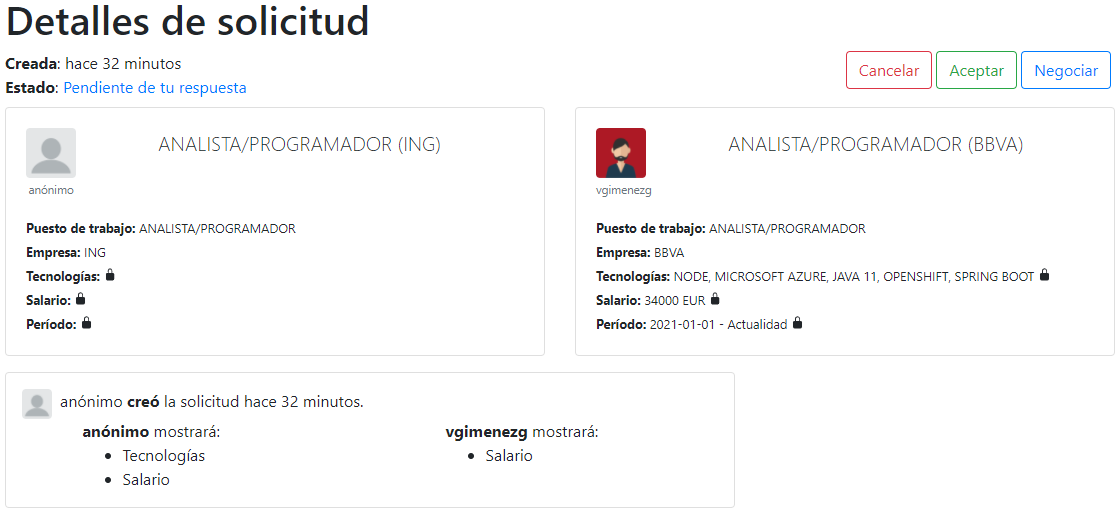
\includegraphics[width=15cm, keepaspectratio]{img/negotiation_details_buttons.PNG}
        \caption{Vista \emph{Detalles de solicitud} durante la negociación.}\label{fig:negotiation_details_buttons}
    \end{figure}

    \begin{figure}
        \centering
        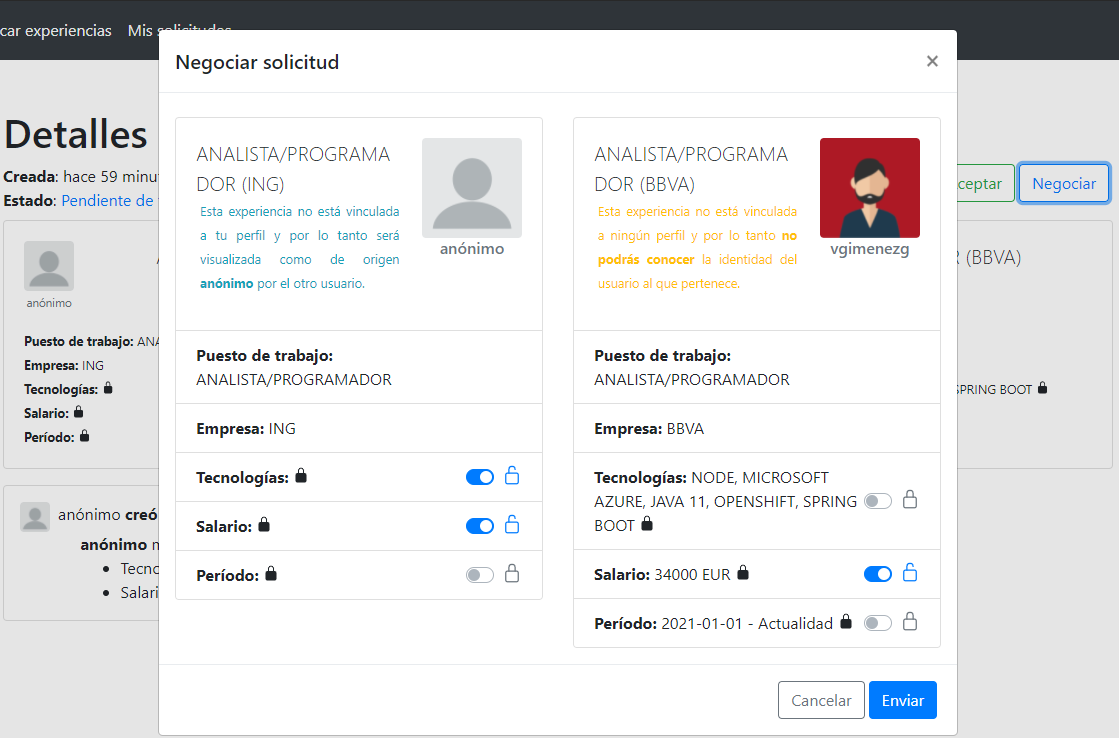
\includegraphics[width=15cm, keepaspectratio]{img/negotiation_details_modal.PNG}
        \caption{Vista \emph{Detalles de solicitud} al modificar las condiciones de la solicitud.}\label{fig:negotiation_details_modal}
    \end{figure}

    \begin{figure}
        \centering
        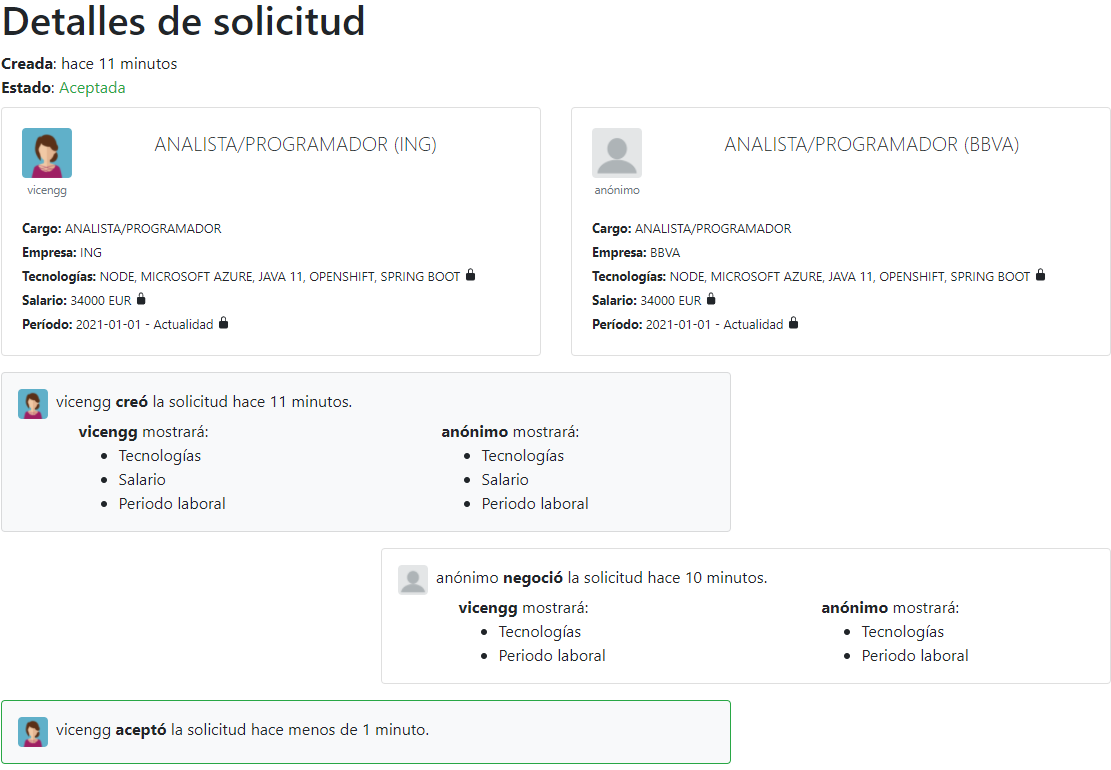
\includegraphics[width=15cm, keepaspectratio]{img/negotiation_details.PNG}
        \caption{Vista \emph{Detalles de solicitud} al concluir la negociación.}\label{fig:negotiation_details}
    \end{figure}


    \section{Casos de uso}
    \label{sec:use_cases}
    En esta sección se procede a describir cada uno de los casos de uso que definen la funcionalidad de la aplicación.
    Estos casos de uso se muestran de forma esquemática en la Figura~\ref{fig:use_cases}.

    \begin{figure}
        \centering
        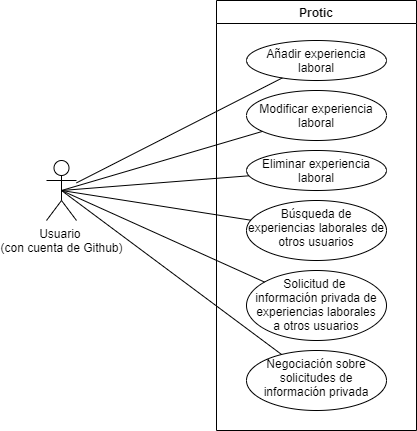
\includegraphics[width=10cm, keepaspectratio]{img/Casos_de_uso.png}
        \caption{Casos de uso de la aplicación.}\label{fig:use_cases}
    \end{figure}

    \subsection{Actores}
    \label{subsec:actors}
    Para describir los casos de uso definiremos dos usuarios de ejemplo, llamados \emph{Usuario 1} y \emph{Usuario 2}.
    Ambos usuarios se registraron en GitHub previamente al ingreso a la aplicación. Para facilitar el seguimiento de los casos
    de uso se especifica que:
    \begin{itemize}
        \item \emph{Usuario 1}: Es un usuario nuevo en la aplicación por lo que no posee experiencias laborales.
        En las figuras que acompañan a la explicación este usuario tendrá el nombre de usuario \emph{vicengg} y un avatar con fondo azul.
        Interviene en todos los casos de uso.
        \item \emph{Usuario 2}: Este usuario ya posee experiencias laborales guardadas en la aplicación.
        En las figuras que acompañan a la explicación este usuario tendrá el nombre de usuario \emph{vgimenezg} y un avatar con fondo rojo.
    \end{itemize}

    \subsection{Antecedentes: Ingreso en la aplicación}
    \label{subsec:background}
    Durante la descripción de los casos de uso, siempre se asumirá que ambos usuarios han realizado los pasos de inicio de sesión
    que se describen a continuación y mantinen su sesión activa a la hora de interactuar en la aplicación:

    \begin{figure}
        \centering
        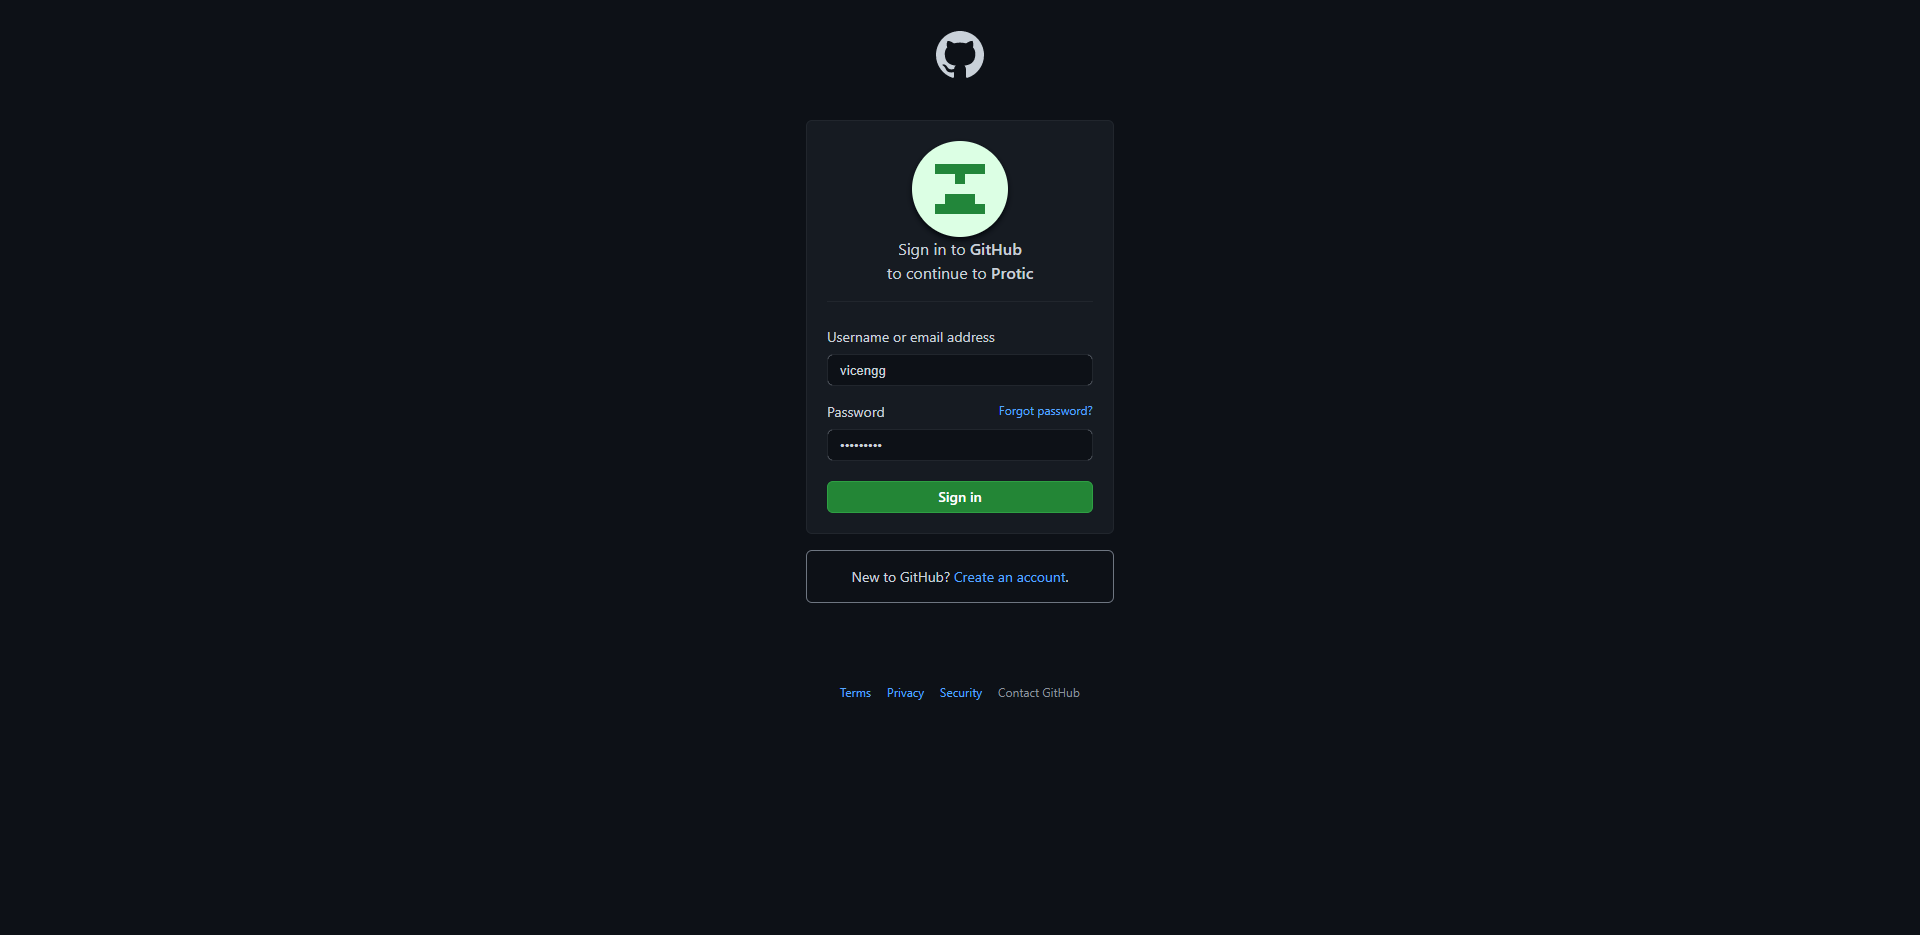
\includegraphics[width=15cm, keepaspectratio]{img/0.1.png}
        \caption{Página de inicio de sesión de GithHub.}\label{fig:use_cases_0_1}
    \end{figure}

    \begin{figure}
        \centering
        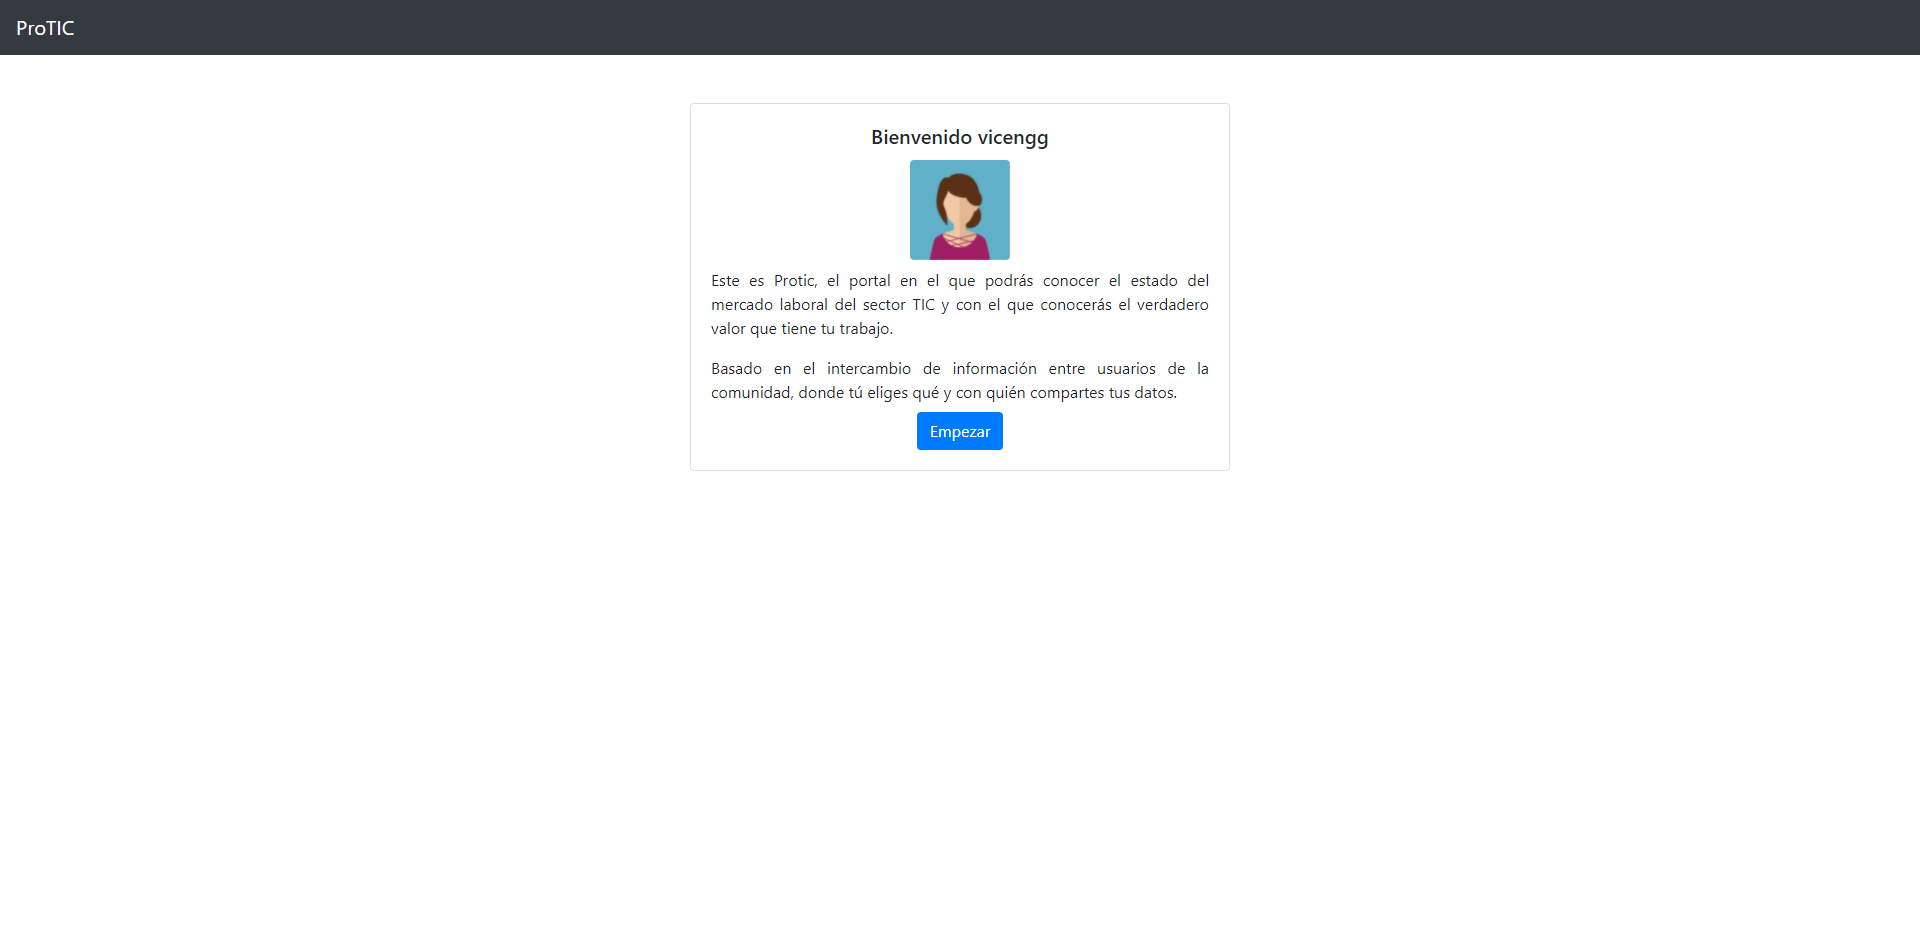
\includegraphics[width=15cm, keepaspectratio]{img/0.2.png}
        \caption{Vista de bienvenida de la aplicación.}\label{fig:use_cases_0_2}
    \end{figure}

    \begin{enumerate}
        \item El usuario fuera de sesión trata de acceder a la vista de bienvenida de la aplicación y es redirigido a la página de inicio de
        sesión de GitHub (Figura~\ref{fig:use_cases_0_1}).
        \item El usuario introduce sus credenciales de GitHub, hace click en el botón \emph{Sign in}
        y es redirigido a la vista de bienvenida de la aplicación (Figura~\ref{fig:use_cases_0_2}).
        \item El usuario hace click en el botón \emph{Empezar}
        y es redirigido a la vista de \emph{Mis experiencias} donde puede acceder a la barra de navegación.
    \end{enumerate}

    \subsection{Añadir experiencia laboral}
    \label{subsec:add_work_experience}
    Para este escenario, el \emph{Usuario 1} ha realizado los pasos que figuran el la Subsección~\ref{subsec:background}
    por lo que su sesión está iniciada y se encuentra en la vista \emph{Mis experiencias} (Figura~\ref{fig:use_cases_1_1}).

    \begin{figure}
        \centering
        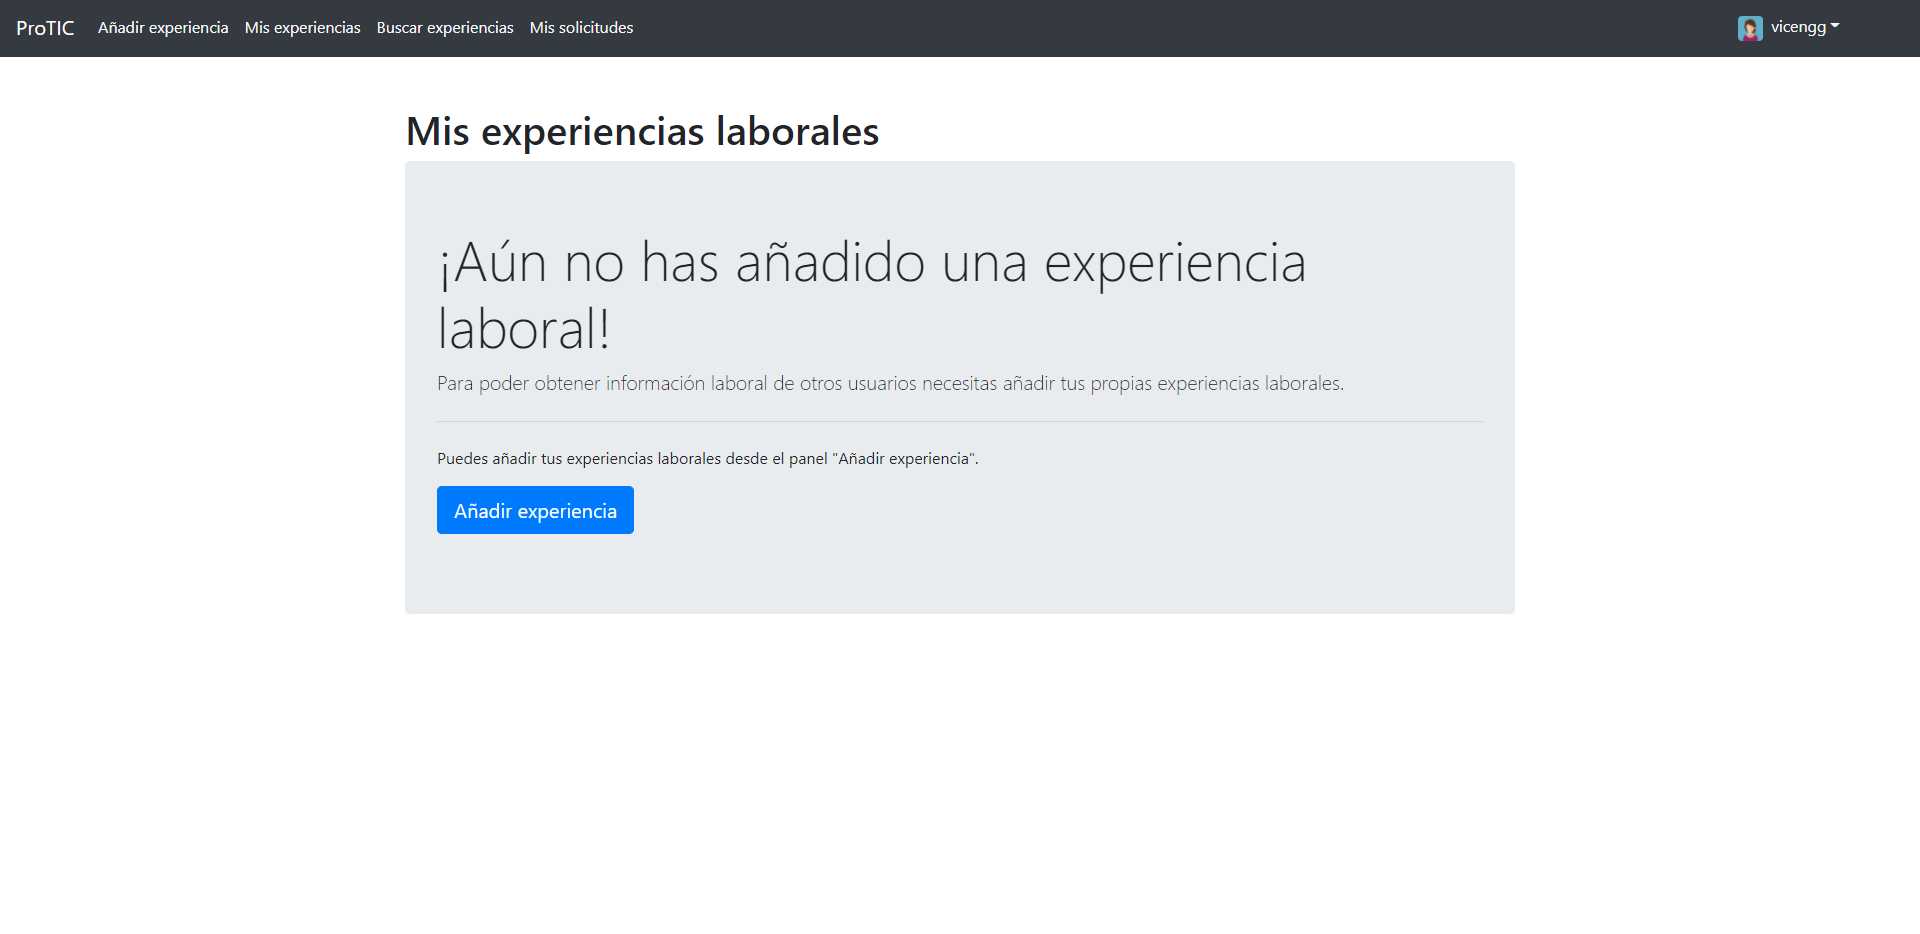
\includegraphics[width=15cm, keepaspectratio]{img/1.1.png}
        \caption{El \emph{Usuario 1} está en la vista \emph{Mis experiencias}.}
        \label{fig:use_cases_1_1}
    \end{figure}

    \begin{figure}
        \centering
        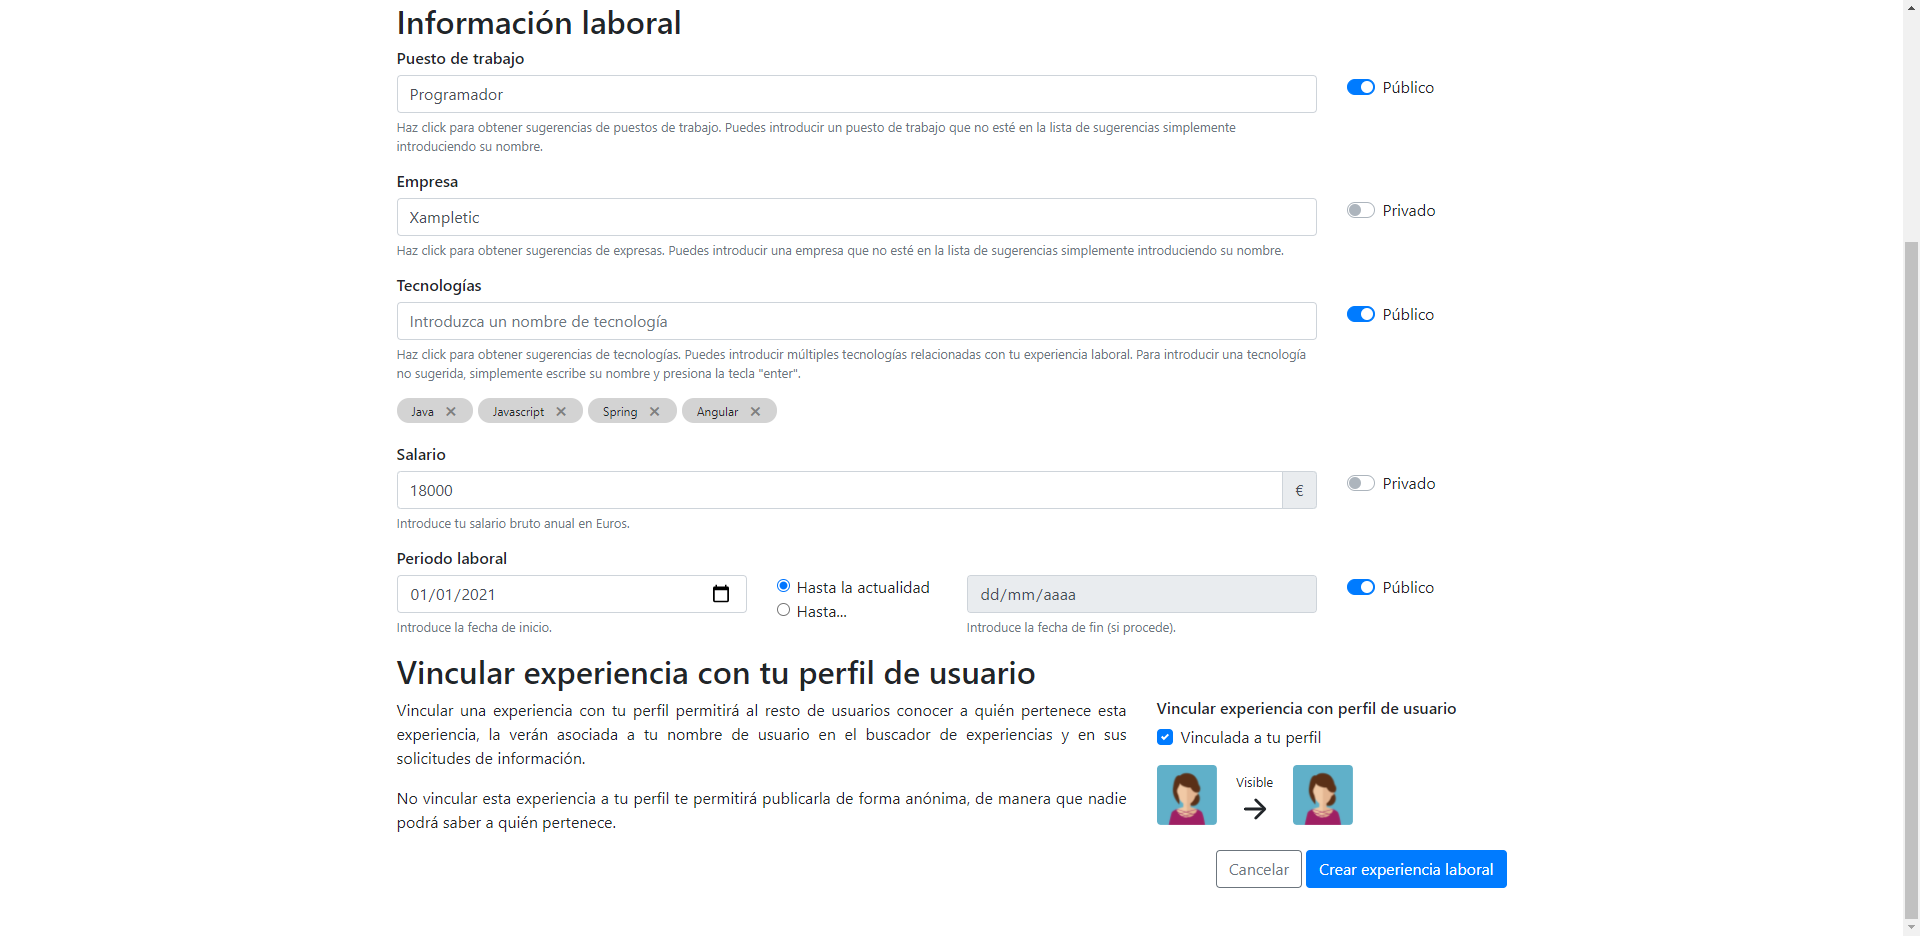
\includegraphics[width=15cm, keepaspectratio]{img/1.2.png}
        \caption{El \emph{Usuario 1} rellena el formulario con la información de la experiencia.}
        \label{fig:use_cases_1_2}
    \end{figure}

    \begin{figure}
        \centering
        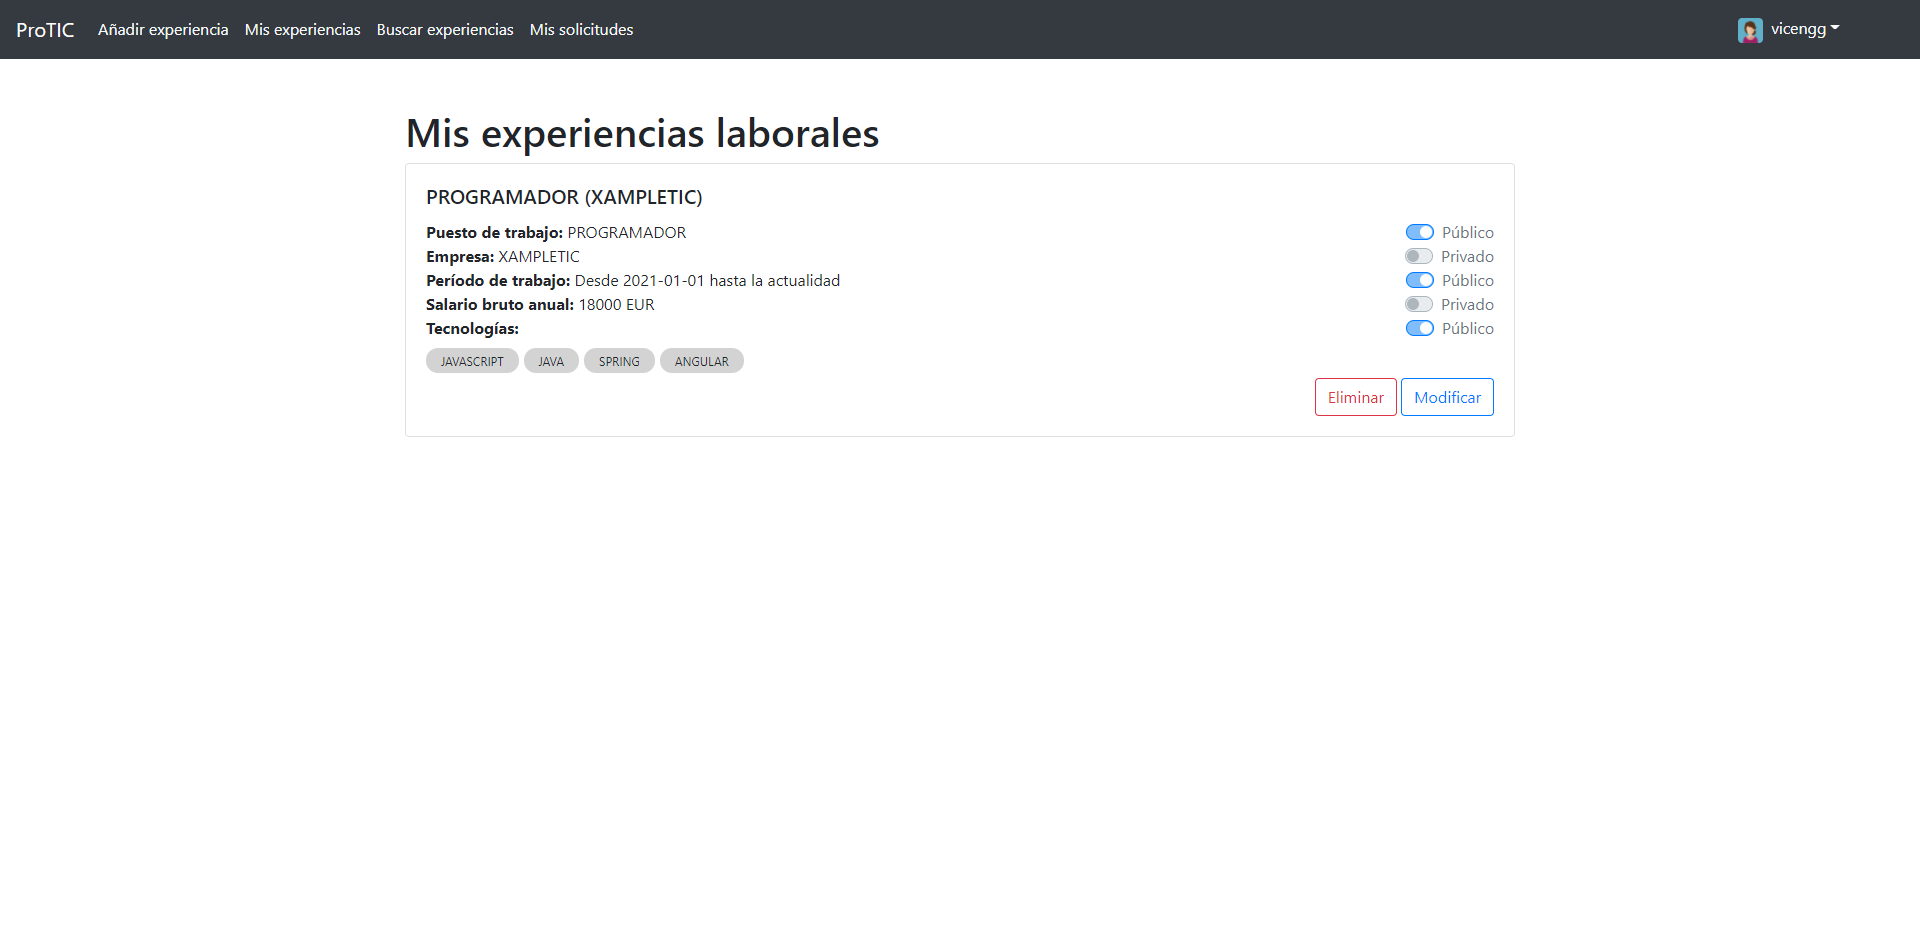
\includegraphics[width=15cm, keepaspectratio]{img/1.3.png}
        \caption{El \emph{Usuario 1} ve su experiencia laboral añadida.}
        \label{fig:use_cases_1_3}
    \end{figure}

    \begin{enumerate}
        \item El \emph{Usuario 1} hace click en el botón \emph{Añadir experiencia}
        (en la barra de navegación o en el mensaje de la pantalla) y navega a la vista \emph{Añadir experiencia}.
        \item El \emph{Usuario 1} rellena el formulario con la información de la experiencia laboral que quiere añadir
        (Figura~\ref{fig:use_cases_1_2}).
        \item El \emph{Usuario 1} elige la visibilidad que desea para cada uno de los campos de su experiencia laboral,
        pública o privada.
        \item El \emph{Usuario 1} elige si quiere vincular la experiencia laboral a su perfil o prefiere
        que figure como anónima para el resto de usuarios.
        \item El \emph{Usuario 1} hace click en el botón \emph{Crear experiencia laboral} y es redirigido de nuevo a la vista
        \emph{Mis experiencias} donde puede ver su nueva experiencia laboral añadida (Figura~\ref{fig:use_cases_1_3}).
    \end{enumerate}

    \subsection{Modificar experiencia laboral}
    \label{subsec:modify_work_experience}
    Para este escenario, el \emph{Usuario 1} ha creado al menos una experiencia laboral como se muestra en la Subsección~\ref{subsec:add_work_experience}
    y se encuentra en la vista \emph{Mis experiencias} (Figura~\ref{fig:use_cases_1_3}) con experiencias en su lista.

    \begin{figure}
        \centering
        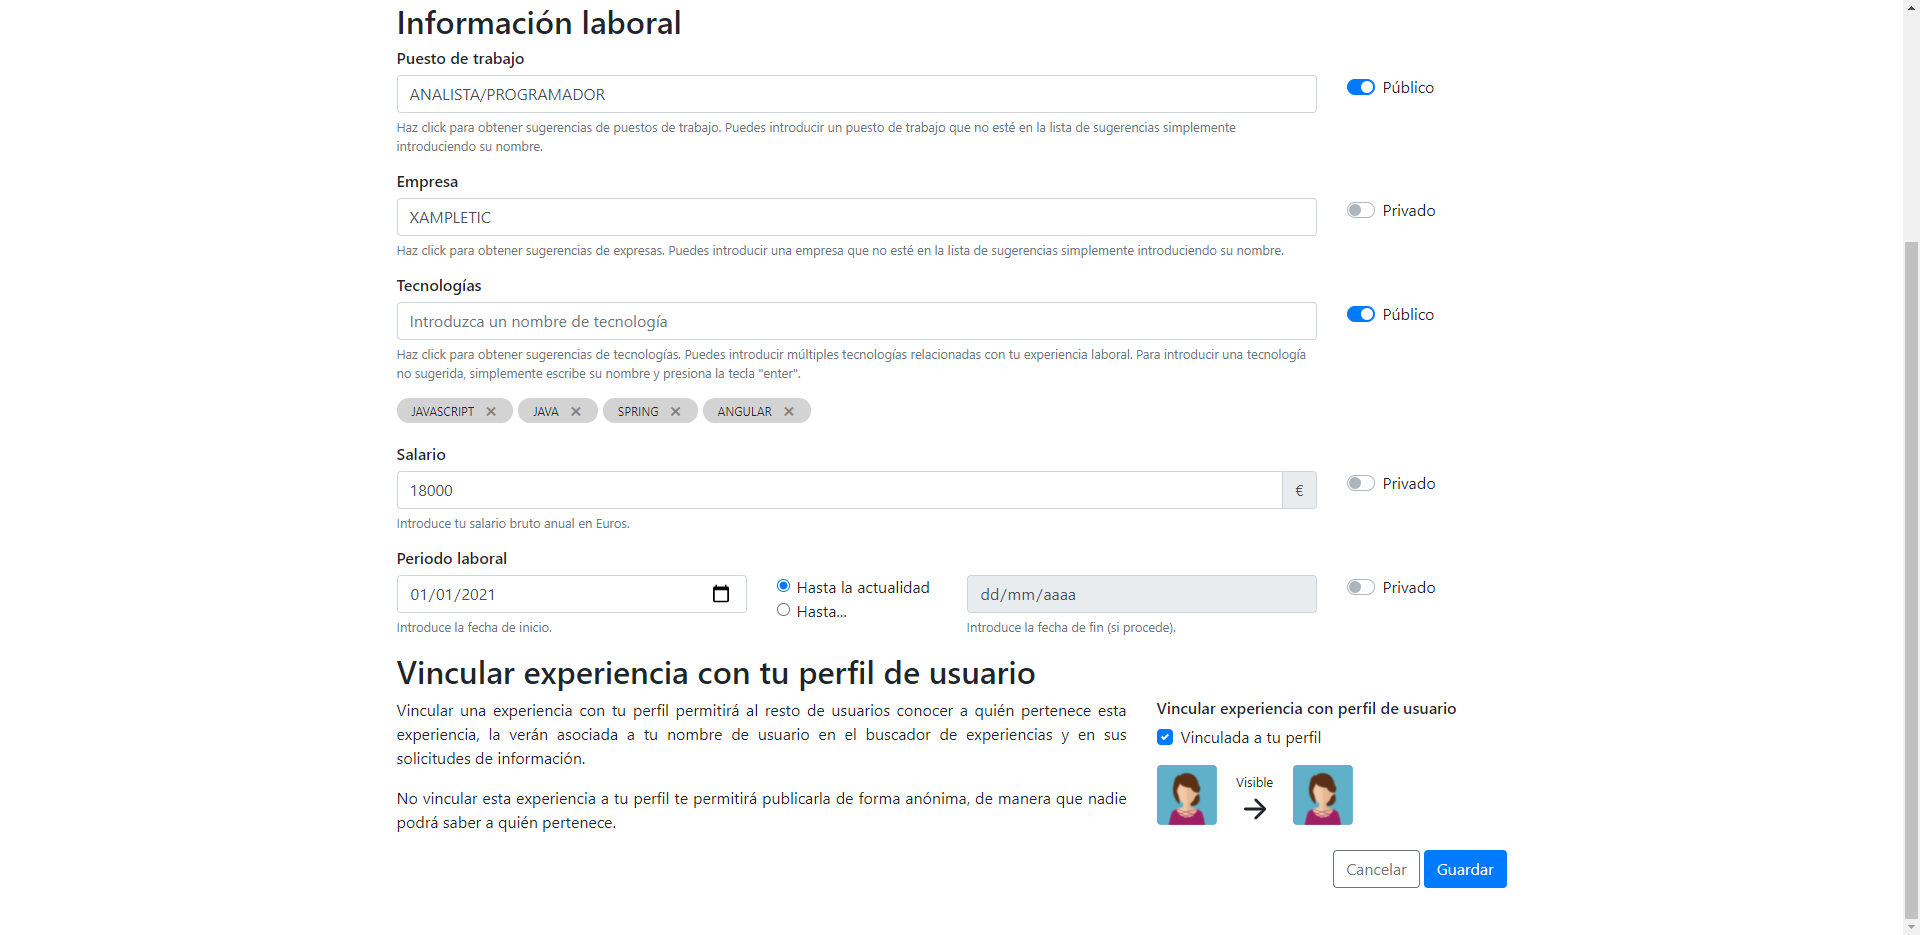
\includegraphics[width=15cm, keepaspectratio]{img/2.1.png}
        \caption{El \emph{Usuario 1} modifica los campos de su experiencia.}
        \label{fig:use_cases_2_1}
    \end{figure}

    \begin{figure}
        \centering
        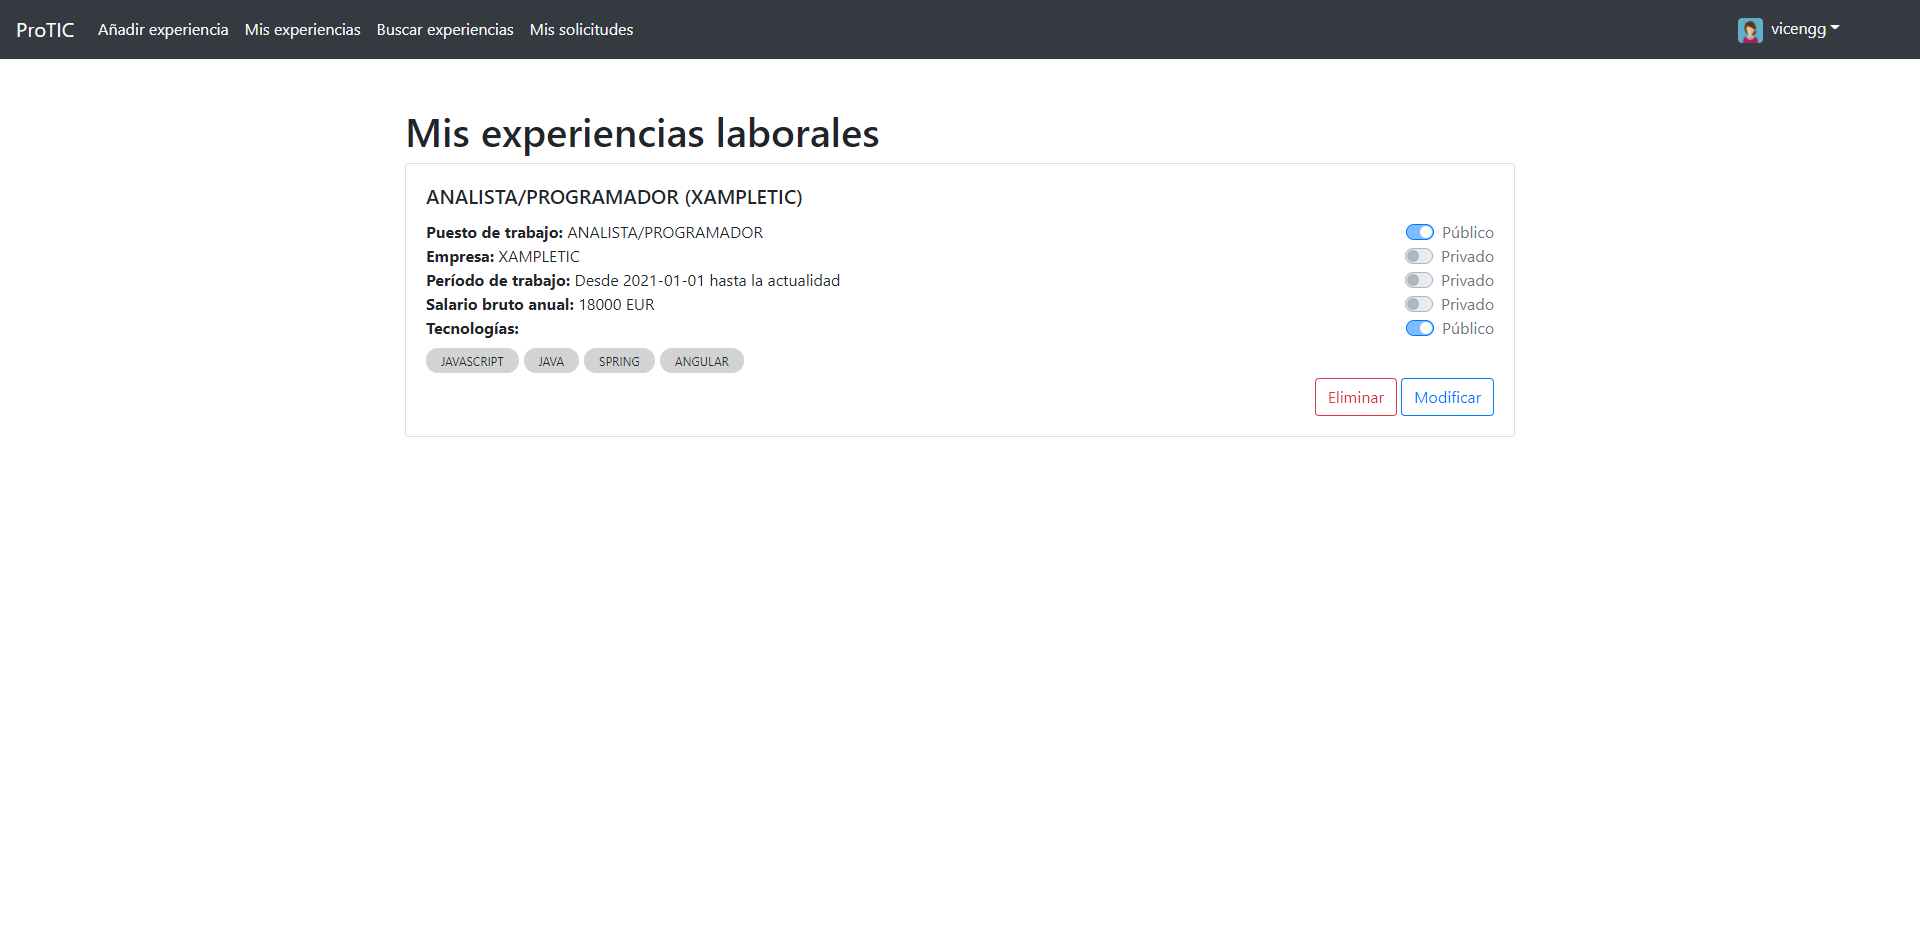
\includegraphics[width=15cm, keepaspectratio]{img/2.2.png}
        \caption{El \emph{Usuario 1} ve su experiencia laboral modificada.}
        \label{fig:use_cases_2_2}
    \end{figure}

    \begin{enumerate}
        \item El \emph{Usuario 1} hace click en el botón \emph{Modificar} y navega a la vista \emph{Editar experiencia}.
        \item El \emph{Usuario 1} modifica en el formulario los campos de su experiencia que desea editar.
        (Figura~\ref{fig:use_cases_2_1}).
        \item El \emph{Usuario 1} modifica las visibilidades que considera para sus campos.
        \item El \emph{Usuario 1} elige de nuevo si quiere vincular la experiencia laboral a su perfil o prefiere
        que figure como anónima para el resto de usuarios.
        \item El \emph{Usuario 1} hace click en el botón \emph{Guardar} y es redirigido a la vista
        \emph{Mis experiencias} donde puede ver su experiencia laboral modificada (Figura~\ref{fig:use_cases_2_2}).
    \end{enumerate}

    \subsection{Eliminar experiencia laboral}
    \label{subsec:delete_work_experience}
    Para este escenario, el \emph{Usuario 1} ha creado al menos una experiencia laboral como se muestra en la Subsección~\ref{subsec:add_work_experience}
    y se encuentra en la vista \emph{Mis experiencias} (Figura~\ref{fig:use_cases_1_3}) con experiencias en su lista.

    \begin{figure}
        \centering
        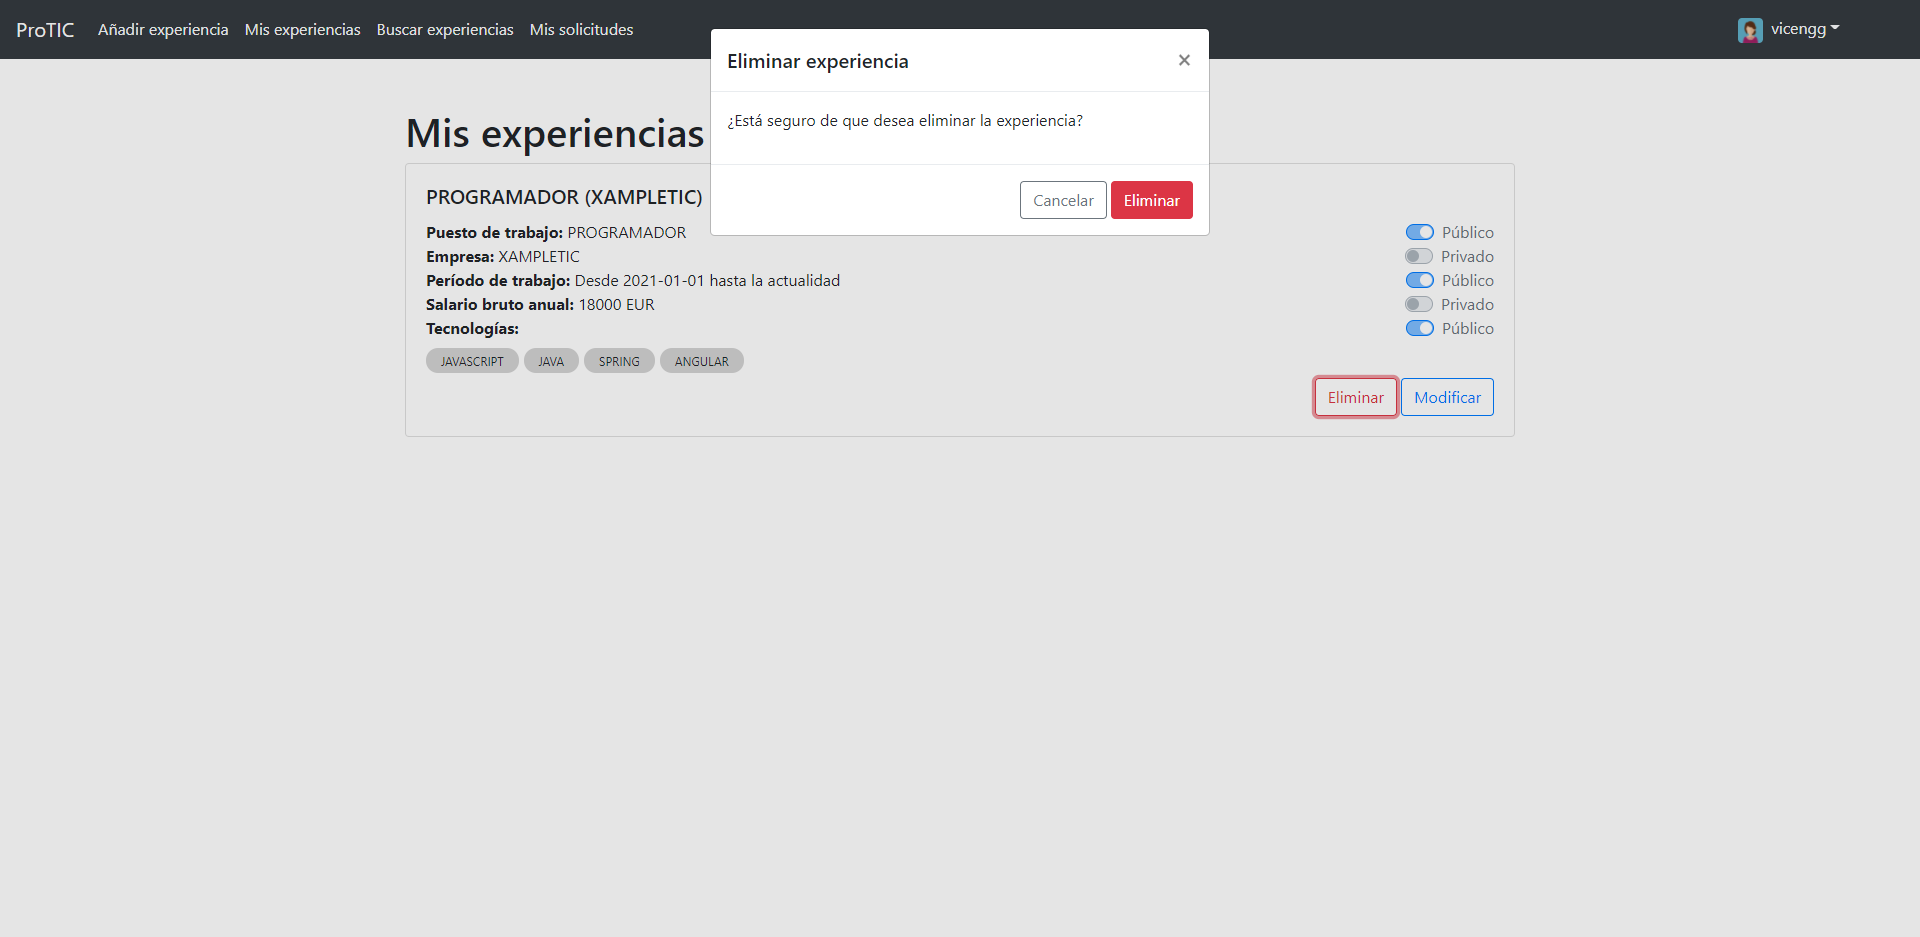
\includegraphics[width=15cm, keepaspectratio]{img/3.1.png}
        \caption{El \emph{Usuario 1} confirma el borrado de su experiencia.}
        \label{fig:use_cases_3_1}
    \end{figure}

    \begin{figure}
        \centering
        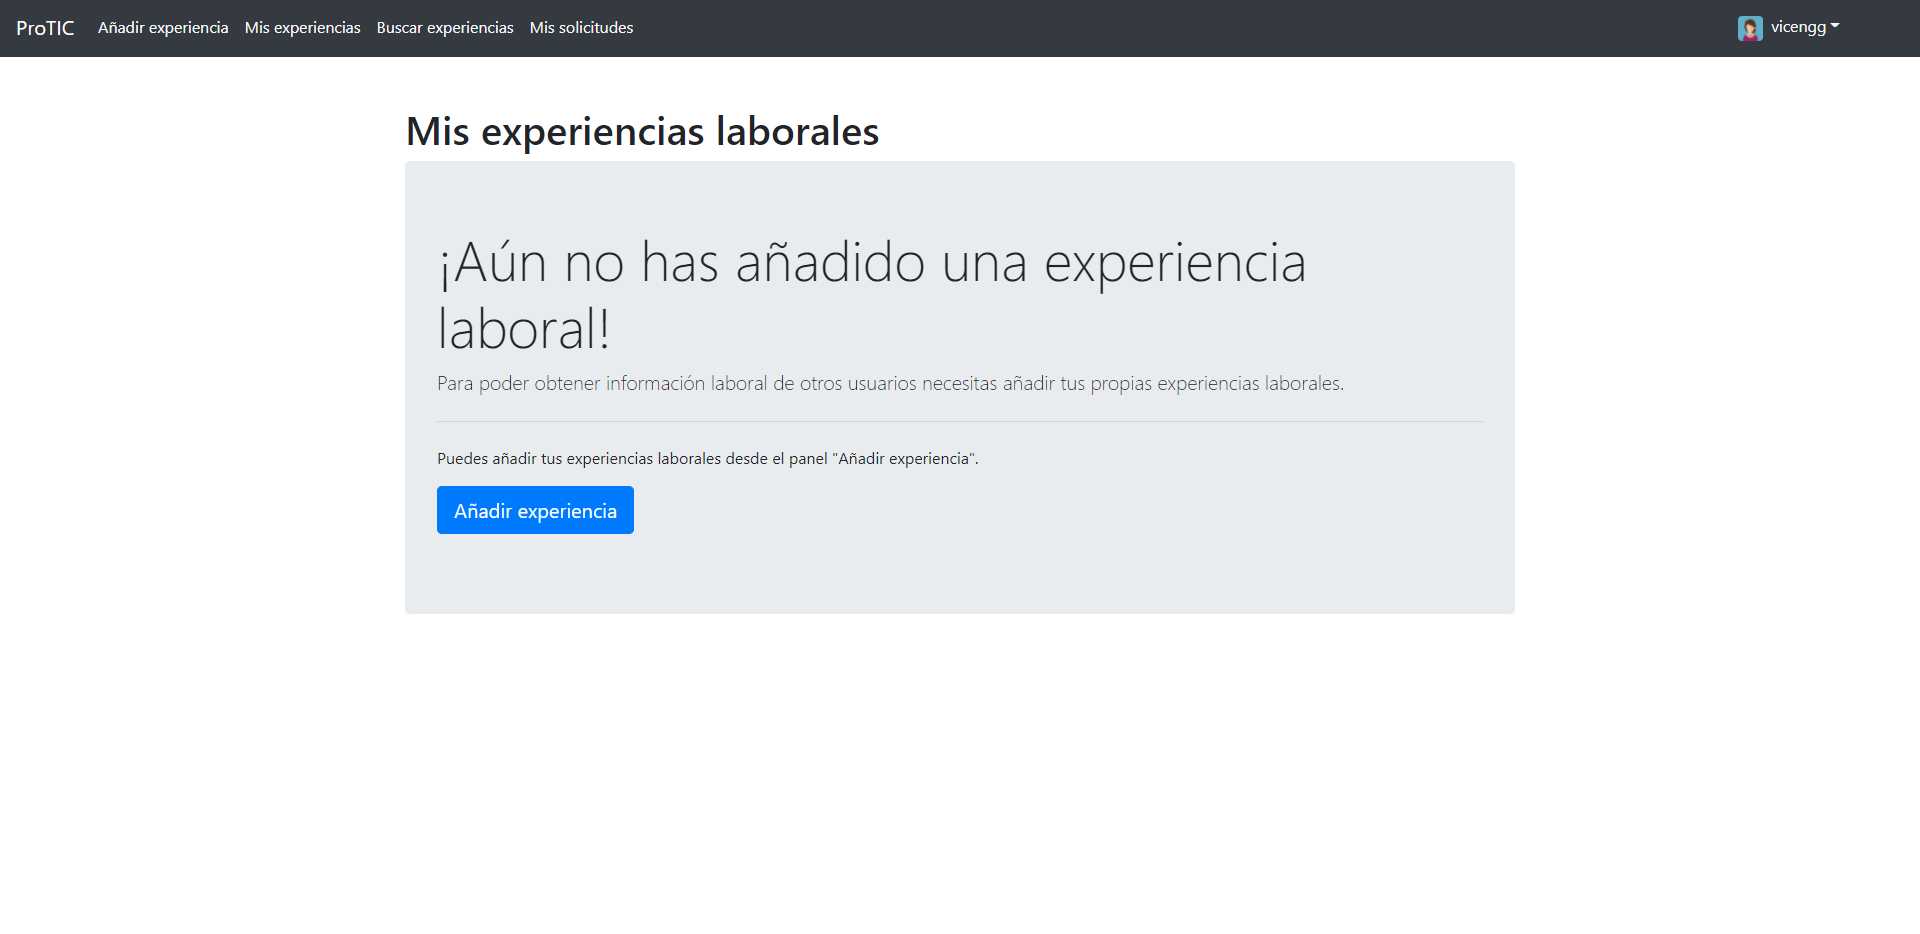
\includegraphics[width=15cm, keepaspectratio]{img/1.1.png}
        \caption{El \emph{Usuario 1} ve que su experiencia laboral ha sido borrada.}
        \label{fig:use_cases_3_2}
    \end{figure}

    \begin{enumerate}
        \item El \emph{Usuario 1} hace click en el botón \emph{Eliminar} y un modal de confirmación aparece en pantalla.
        \item El \emph{Usuario 1} confirma el borrado haciendo click en el botón \emph{Eliminar} del modal.
        (Figura~\ref{fig:use_cases_3_1}).
        \item El modal se cierra y el contenido de la vista se actualiza para mostrar que la experiencia laboral ha sido eliminada (Figura~\ref{fig:use_cases_3_2}).
    \end{enumerate}

    \subsection{Búsqueda de experiencias laborales de otros usuarios}
    \label{subsec:search_work_experiences}
    Para este escenario, el \emph{Usuario 1} ha realizado los pasos que figuran el la Subsección~\ref{subsec:background}
    por lo que su sesión está iniciada y desde la barra de navegación accede a la vista \emph{Buscar experiencias}
    (Figura~\ref{fig:use_cases_4_1}).

    \begin{figure}
        \centering
        \includegraphics[width=15cm, keepaspectratio]{img/4.1.png}
        \caption{El \emph{Usuario 1} está en la vista \emph{Buscar experiencias}.}
        \label{fig:use_cases_4_1}
    \end{figure}

    \begin{figure}
        \centering
        \includegraphics[width=15cm, keepaspectratio]{img/4.2.png}
        \caption{El \emph{Usuario 1} filtra la búsqueda.}
        \label{fig:use_cases_4_2}
    \end{figure}

    \begin{enumerate}
        \item El \emph{Usuario 1} rellena los filtros en la parte superior de la pantalla para realizar
        una búsqueda de las experiencias que le interesan.
        \item Cuando los filtros se rellenan la información de la pagína se actualiza automáticamente
        para mostrar los resultados (Figura~\ref{fig:use_cases_4_2}).
    \end{enumerate}

    \subsection{Solicitud de información privada de experiencias laborales a otros usuarios}
    \label{subsec:search_work_experiences}
    Para este escenario, el \emph{Usuario 1} ha creado al menos una experiencia laboral como se muestra en la Subsección~\ref{subsec:add_work_experience}
    y se encuentra en la vista \emph{Buscar experiencias} (Figura~\ref{fig:use_cases_5_1}) con experiencias en su lista.

    \begin{figure}
        \centering
        \includegraphics[width=15cm, keepaspectratio]{img/5.1.png}
        \caption{El \emph{Usuario 1} está en la vista \emph{Buscar experiencias}.}
        \label{fig:use_cases_5_1}
    \end{figure}

    \begin{figure}
        \centering
        \includegraphics[width=15cm, keepaspectratio]{img/5.2.png}
        \caption{El \emph{Usuario 1} está en la vista \emph{Solicitar información}.}
        \label{fig:use_cases_5_2}
    \end{figure}

    \begin{figure}
        \centering
        \includegraphics[width=15cm, keepaspectratio]{img/5.3.png}
        \caption{El \emph{Usuario 1} está en la vista \emph{Mis solicitudes}.}
        \label{fig:use_cases_5_3}
    \end{figure}

    \begin{figure}
        \centering
        \includegraphics[width=15cm, keepaspectratio]{img/5.4.png}
        \caption{El \emph{Usuario 1} está en la vista \emph{Detalles de solicitud}.}
        \label{fig:use_cases_5_4}
    \end{figure}

    \begin{enumerate}
        \item El \emph{Usuario 1} seleccion una experiencia laboral de otro usuario (\emph{Usuario 2}), hace click en el botón \emph{Solicitar más información}
        y es redirigido a la vista de \emph{Solicitud de información} (Figura~\ref{fig:use_cases_5_2}).
        \item En la parte superior de la tarjeta izquierda, el \emph{Usuario 1} selecciona la experiencia laboral que desea ofrecer en el seleccionable.
        \item En la parte inferior de la tarjeta izquierda, el \emph{Usuario 1} elige los campos de su experiencia que está dispuesto a ofrecer al \emph{Usuario 2}.
        \item En la parte inferior de la tarjeta derecha, el \emph{Usuario 1} elige los campos de la experiencia del \emph{Usuario 2} que desea que le sean revelados.
        \item El \emph{Usuario 1} hace click en el botón \emph{Solicitar información}
        y es redirigido a la vista \emph{Mis solicitudes} (Figura~\ref{fig:use_cases_5_3}) donde puede ver en la lista la entrada relativa a su nueva solicitud.
        \item El \emph{Usuario 1} hace click en el botón \emph{Ver detalles}
        y es redirigido a la vista \emph{Detalles de solicitud} (Figura~\ref{fig:use_cases_5_4}) donde comprueba los detalles de su solicitud recién creada.
    \end{enumerate}

    \subsection{Negociación sobre solicitudes de información privada}
    \label{subsec:search_work_experiences}
    Para este escenario, el \emph{Usuario 1} ha realizado los pasos descritos en la Subsección~\ref{subsec:search_work_experiences}
    por lo que tiene un solicitud de información creada sobre una experiencia laboral del \emph{Usuario 2}.

    \begin{figure}
        \centering
        \includegraphics[width=15cm, keepaspectratio]{img/6.1.png}
        \caption{El \emph{Usuario 2} está en la vista \emph{Mis solicitudes}.}
        \label{fig:use_cases_6_1}
    \end{figure}

    \begin{figure}
        \centering
        \includegraphics[width=15cm, keepaspectratio]{img/6.2.png}
        \caption{El \emph{Usuario 2} está en la vista \emph{Detalles de solicitud}.}
        \label{fig:use_cases_6_2}
    \end{figure}

    \begin{figure}
        \centering
        \includegraphics[width=15cm, keepaspectratio]{img/6.3.png}
        \caption{El \emph{Usuario 2} negocia los términos de la solictud en la ventana modal.}
        \label{fig:use_cases_6_3}
    \end{figure}

    \begin{figure}
        \centering
        \includegraphics[width=15cm, keepaspectratio]{img/6.4.png}
        \caption{El estado de la solicitud cambia a pendiente de la respuesta del \emph{Usuario 1}.}
        \label{fig:use_cases_6_4}
    \end{figure}

    \begin{figure}
        \centering
        \includegraphics[width=15cm, keepaspectratio]{img/6.5.png}
        \caption{El \emph{Usuario 1} visualiza el cambio en el histórico de la solcitud.}
        \label{fig:use_cases_6_5}
    \end{figure}

    \begin{figure}
        \centering
        \includegraphics[width=15cm, keepaspectratio]{img/6.6.png}
        \caption{El \emph{Usuario 1} acepta la solicitud y puede ver los campos de las experiencias desvelados.}
        \label{fig:use_cases_6_6}
    \end{figure}

    \begin{enumerate}
        \item El \emph{Usuario 2} accede desde la barra de navegación a la vista \emph{Mis solicitudes},
        donde una solicitud aparece con el estado \emph{Pendiente de tu respuestas} (Figura~\ref{fig:use_cases_6_1}).
        \item El \emph{Usuario 2} hace click en el botón \emph{Ver detalles} y es redirigido
        a la vista \emph{Detalles de solicitud} (Figura~\ref{fig:use_cases_6_2}).
        \item El \emph{Usuario 2} hace click en el botón \emph{Negociar} y emerge una ventana modal que le permite modificar
        los términos de la solicitud (Figura~\ref{fig:use_cases_6_3}).
        \item El \emph{Usuario 2} hace click en el botón \emph{Enviar} para cambiar los términos de la negociación,
        y la solicitud pasa ahora al estado pendiente de respuesta por parte del \emph{Usuario 1} (Figura~\ref{fig:use_cases_6_4}).
        Esta nueva opción se refleja automáticamente en el histórico de la solicitud en la parte inferior de la vista.
        Los pasos 3 y 4 son opcionales, y se pueden repetir un número indeterminado de veces alternando el turno
        entre el \emph{Usuario 1} y el \emph{Usuario 2}. Cada nueva negociación se añadirá al histórico.
        \item El \emph{Usuario 1} accede a la vista de detalles de la negociación, donde puede ver el nuevo paso en el
        histórico (Figura~\ref{fig:use_cases_6_5}).
        \item El \emph{Usuario 1} hace click en el botón \emph{Aceptar} para aceptar los nuevos términos de la solicitud, inmediatamente
        la vista se recarga mostrando los campos desvelados de la experiencia laboral del \emph{Usuario 2} (Figura~\ref{fig:use_cases_6_6}).
        \item El \emph{Usuario 2} del mismo modo puede comprobar los campos desvelados de la experiencia del \emph{Usuario 1}.
    \end{enumerate}

    En cualquier momento de este proceso previo a la aceptación ambos usuarios podrían cancelar la solicitud.


%%%%%%%%%%%%%%%%%%%%%%%%%%%%%%%%%%%%%%%%%%%%%%%%%%%%%%%%%%%%%%%%%%%%%%%%%%%%%%%%
%%%%%%%%%%%%%%%%%%%%%%%%%%%%%%%%%%%%%%%%%%%%%%%%%%%%%%%%%%%%%%%%%%%%%%%%%%%%%%%%
% EXPERIMENTOS Y VALIDACIÓN %
%%%%%%%%%%%%%%%%%%%%%%%%%%%%%%%%%%%%%%%%%%%%%%%%%%%%%%%%%%%%%%%%%%%%%%%%%%%%%%%%

    \cleardoublepage
    \chapter{Experimentos y validación}

    [TODO]


%%%%%%%%%%%%%%%%%%%%%%%%%%%%%%%%%%%%%%%%%%%%%%%%%%%%%%%%%%%%%%%%%%%%%%%%%%%%%%%%
%%%%%%%%%%%%%%%%%%%%%%%%%%%%%%%%%%%%%%%%%%%%%%%%%%%%%%%%%%%%%%%%%%%%%%%%%%%%%%%%
% RESULTADOS %
%%%%%%%%%%%%%%%%%%%%%%%%%%%%%%%%%%%%%%%%%%%%%%%%%%%%%%%%%%%%%%%%%%%%%%%%%%%%%%%%

    \cleardoublepage
    \chapter{Resultados}

    {\footnotesize
        \begin{verbatim}
Feature: Work experience visibility by default
  Check the work experiences visibility business rules by default.

  Background:
    Given a user with id "user_1"
    And a user with id "user_2"
    And the user "user_1" starts to fill the create work experience form

  Scenario: User 1 creates a work experience associated to his profile with all fields public.
    When the user "user_1" fills the job title as "developer" with "public" visibility
    And the user "user_1" fills the company as "Google" with "public" visibility
    And the user "user_1" adds a technology "Java" with "public" visibility
    And the user "user_1" adds a work period from "2016-08-16" to present with "public" visibility
    And the user "user_1" adds a salary of 50000 "EUR" with "public" visibility
    And the user "user_1" sends his work experience to create, associated to his profile, with reference ID "work_experience_1"
    When the user "user_1" gets his own work experiences
    Then the work experience "work_experience_1" is present
    And the work experience job title is present
    And the work experience company is present
    And the work experience technologies are present
    And the work experience work period is present
    And the work experience salary is present
    And the work experience user is NOT anonymous

  Scenario: User 1 creates a work experience anonymously with all fields private, but he can see all data.
    When the user "user_1" fills the job title as "developer" with "private" visibility
    And the user "user_1" fills the company as "Google" with "private" visibility
    And the user "user_1" adds a technology "Java" with "private" visibility
    And the user "user_1" adds a work period from "2016-08-16" to present with "private" visibility
    And the user "user_1" adds a salary of 50000 "EUR" with "private" visibility
    And the user "user_1" sends his work experience to create, anonymously, with reference ID "work_experience_1"
    When the user "user_1" gets his own work experiences
    Then the work experience "work_experience_1" is present
    And the work experience job title is present
    And the work experience company is present
    And the work experience technologies are present
    And the work experience work period is present
    And the work experience salary is present
    And the work experience user is NOT anonymous

  Scenario: User 1 creates a work experience associated to his profile with all fields public, then User 2 can see all data.
    When the user "user_1" fills the job title as "developer" with "public" visibility
    And the user "user_1" fills the company as "Google" with "public" visibility
    And the user "user_1" adds a technology "Java" with "public" visibility
    And the user "user_1" adds a work period from "2016-08-16" to present with "public" visibility
    And the user "user_1" adds a salary of 50000 "EUR" with "public" visibility
    And the user "user_1" sends his work experience to create, associated to his profile, with reference ID "work_experience_1"
    When the user "user_2" gets his own work experiences
    Then the work experience "work_experience_1" is NOT present
    When the user "user_2" gets work experiences of others
    Then the work experience "work_experience_1" is present
    And the work experience job title is present
    And the work experience company is present
    And the work experience technologies are present
    And the work experience work period is present
    And the work experience salary is present
    And the work experience user is NOT anonymous

  Scenario: User 1 creates a work experience anonymously with all fields private, then User 2 can't see any field nor the owner identity.
    When the user "user_1" fills the job title as "developer" with "private" visibility
    And the user "user_1" fills the company as "Google" with "private" visibility
    And the user "user_1" adds a technology "Java" with "private" visibility
    And the user "user_1" adds a work period from "2016-08-16" to present with "private" visibility
    And the user "user_1" adds a salary of 50000 "EUR" with "private" visibility
    And the user "user_1" sends his work experience to create, anonymously, with reference ID "work_experience_1"
    When the user "user_2" gets his own work experiences
    Then the work experience "work_experience_1" is NOT present
    When the user "user_2" gets work experiences of others
    Then the work experience "work_experience_1" is present
    And the work experience job title is NOT present
    And the work experience company is NOT present
    And the work experience technologies are NOT present
    And the work experience work period is NOT present
    And the work experience salary is NOT present
    And the work experience user is anonymous

        \end{verbatim}
    }

    {\footnotesize
        \begin{verbatim}
Feature: Work experience visibility with negotiations
  Check the work experiences visibility business rules with negotiation.

  Background:
    Given a user with id "user_1"
    And a user with id "user_2"
    And the user "user_1" starts to fill the create work experience form
    And the user "user_1" fills the job title as "developer" with "private" visibility
    And the user "user_1" fills the company as "Google" with "private" visibility
    And the user "user_1" adds a technology "Java" with "private" visibility
    And the user "user_1" adds a work period from "2016-08-16" to present with "private" visibility
    And the user "user_1" adds a salary of 50000 "EUR" with "private" visibility
    And the user "user_1" sends his work experience to create, anonymously, with reference ID "work_experience_1"
    And the user "user_2" starts to fill the create work experience form
    And the user "user_2" fills the job title as "developer" with "private" visibility
    And the user "user_2" fills the company as "Amazon" with "private" visibility
    And the user "user_2" adds a technology "JavaScript" with "private" visibility
    And the user "user_2" adds a work period from "2017-05-12" to present with "private" visibility
    And the user "user_2" adds a salary of 60000 "EUR" with "private" visibility
    And the user "user_2" sends his work experience to create, anonymously, with reference ID "work_experience_2"

  Scenario: Without negotiation, User 2 can't see anything about User 1's experience
    When the user "user_2" gets work experiences of others
    Then the work experience "work_experience_1" is present
    And the work experience job title is NOT present
    And the work experience company is NOT present
    And the work experience technologies are NOT present
    And the work experience work period is NOT present
    And the work experience salary is NOT present
    And the work experience user is anonymous

  Scenario:User 2 creates a negotiation asking for visibility for all fields and offering all the fields of his work experience
    When the user "user_2" creates a data request to unlock "work_experience_1" offering "work_experience_2"
    And the user "user_2" adds a negotiation step
    And asks for visibility for "job title, company, technologies, work period and salary"
    And offers visibility for "job title, company, technologies, work period and salary"
    And "user_2" sends the negotiation
    And "user_1" accepts the negotiation
    When the user "user_2" gets work experiences of others
    Then the work experience "work_experience_1" is present
    And the work experience job title is present
    And the work experience company is present
    And the work experience technologies are present
    And the work experience work period is present
    And the work experience salary is present
    And the work experience user is anonymous
    When the user "user_1" gets work experiences of others
    Then the work experience "work_experience_2" is present
    And the work experience job title is present
    And the work experience company is present
    And the work experience technologies are present
    And the work experience work period is present
    And the work experience salary is present
    And the work experience user is anonymous

  Scenario: User 2 creates a negotiation asking for visibility for some fields of the User 1's work experience and offering some fields of his work experience
    When the user "user_2" creates a data request to unlock "work_experience_1" offering "work_experience_2"
    And the user "user_2" adds a negotiation step
    And asks for visibility for "job title, work period and salary"
    And offers visibility for "company and technologies"
    And "user_2" sends the negotiation
    And "user_1" accepts the negotiation
    When the user "user_2" gets work experiences of others
    Then the work experience "work_experience_1" is present
    And the work experience job title is present
    And the work experience company is NOT present
    And the work experience technologies are NOT present
    And the work experience work period is present
    And the work experience salary is present
    And the work experience user is anonymous
    When the user "user_1" gets work experiences of others
    Then the work experience "work_experience_2" is present
    And the work experience job title is NOT present
    And the work experience company is present
    And the work experience technologies are present
    And the work experience work period is NOT present
    And the work experience salary is NOT present
    And the work experience user is anonymous


        \end{verbatim}
    }


%%%%%%%%%%%%%%%%%%%%%%%%%%%%%%%%%%%%%%%%%%%%%%%%%%%%%%%%%%%%%%%%%%%%%%%%%%%%%%%%
%%%%%%%%%%%%%%%%%%%%%%%%%%%%%%%%%%%%%%%%%%%%%%%%%%%%%%%%%%%%%%%%%%%%%%%%%%%%%%%%
% CONCLUSIONES %
%%%%%%%%%%%%%%%%%%%%%%%%%%%%%%%%%%%%%%%%%%%%%%%%%%%%%%%%%%%%%%%%%%%%%%%%%%%%%%%%

    \cleardoublepage


    \chapter{Conclusiones}
    \label{chap:conclusiones}


    \section{Consecución de objetivos}
    \label{sec:consecucion-objetivos}

    [TODO]


    \section{Aplicación de lo aprendido}
    \label{sec:aplicacion}

    [TODO]


    \section{Lecciones aprendidas}
    \label{sec:lecciones_aprendidas}

    [TODO]


    \section{Trabajos futuros}
    \label{sec:trabajos_futuros}

    Para posibles fases posteriores a este Trabajo Fin de Grado se proponen los siguientes trabajos que podrían mejorar la aplicación:

    \begin{itemize}
        \item Agregar a la aplicación una tecnología de generación de contenedores, como Docker, que permita desplegar
        el servidor de aplicaciones, la aplicación web y la base de datos en un servidor accesible desde internet fácilmente.
        \item Añadir integración vía OAuth con LinkedIn adicionalmente a GitHub, de forma que los usuarios con cuenta de LinkedIn también puedan acceder a la aplicación,
        lo que haría la funcionalidad más accesible a usuarios que no fueran del sector TIC.
        \item Hacer la aplicación totalmente responsiva en dispositivos móviles.
        A pesar de que la aplicación está preparada para poder ser utilizada en dispositivos móviles sería posible mejorar la experiencia de usuario
        aplicando un diseño más amistoso para este tipo de dispositivos.
        \item Añadir validaciones en la interfaz de usuario de formato y obligatoriedad para la creación y modificación de experiencias.
        Se podría modificar los componentes que sirven de entrada de datos en los formularios para que estos mostraran errores al usuario
        caso de que falten campos obligatorios o no se hayan introducido en el formato correcto.
        \item Mostrar notificaciones cuando hay solicitudes de información nuevas en un punto de la aplicación que sea observable desde cualquier vista, como la barra de navegación.
        \item Añadir una descripción al modelo de experiencia laboral para poder intercambiar también información cualitativa.
        \item Implementar una funcionalidad de limpieza de filtros en la vista de búsqueda de experiencias laborales.
    \end{itemize}


%%%%%%%%%%%%%%%%%%%%%%%%%%%%%%%%%%%%%%%%%%%%%%%%%%%%%%%%%%%%%%%%%%%%%%%%%%%%%%%%
%%%%%%%%%%%%%%%%%%%%%%%%%%%%%%%%%%%%%%%%%%%%%%%%%%%%%%%%%%%%%%%%%%%%%%%%%%%%%%%%
% APÉNDICE(S) %
%%%%%%%%%%%%%%%%%%%%%%%%%%%%%%%%%%%%%%%%%%%%%%%%%%%%%%%%%%%%%%%%%%%%%%%%%%%%%%%%

    \cleardoublepage
    \appendix


    \chapter{Manual de usuario}
    \label{app:manual}

    [TODO]

%%%%%%%%%%%%%%%%%%%%%%%%%%%%%%%%%%%%%%%%%%%%%%%%%%%%%%%%%%%%%%%%%%%%%%%%%%%%%%%%
%%%%%%%%%%%%%%%%%%%%%%%%%%%%%%%%%%%%%%%%%%%%%%%%%%%%%%%%%%%%%%%%%%%%%%%%%%%%%%%%
% BIBLIOGRAFIA %
%%%%%%%%%%%%%%%%%%%%%%%%%%%%%%%%%%%%%%%%%%%%%%%%%%%%%%%%%%%%%%%%%%%%%%%%%%%%%%%%

    \cleardoublepage

% Las siguientes dos instrucciones es todo lo que necesitas
% para incluir las citas en la memoria
    \bibliographystyle{abbrv}
    \bibliography{memoria}  % memoria.bib es el nombre del fichero que contiene
% las referencias bibliográficas. Abre ese fichero y mira el formato que tiene,
% que se conoce como BibTeX. Hay muchos sitios que exportan referencias en
% formato BibTeX. Prueba a buscar en http://scholar.google.com por referencias
% y verás que lo puedes hacer de manera sencilla.
% Más información: 
% http://texblog.org/2014/04/22/using-google-scholar-to-download-bibtex-citations/

\end{document}
